% Options for packages loaded elsewhere
\PassOptionsToPackage{unicode}{hyperref}
\PassOptionsToPackage{hyphens}{url}
%
\documentclass[
]{book}
\usepackage{amsmath,amssymb}
\usepackage{lmodern}
\usepackage{iftex}
\ifPDFTeX
  \usepackage[T1]{fontenc}
  \usepackage[utf8]{inputenc}
  \usepackage{textcomp} % provide euro and other symbols
\else % if luatex or xetex
  \usepackage{unicode-math}
  \defaultfontfeatures{Scale=MatchLowercase}
  \defaultfontfeatures[\rmfamily]{Ligatures=TeX,Scale=1}
\fi
% Use upquote if available, for straight quotes in verbatim environments
\IfFileExists{upquote.sty}{\usepackage{upquote}}{}
\IfFileExists{microtype.sty}{% use microtype if available
  \usepackage[]{microtype}
  \UseMicrotypeSet[protrusion]{basicmath} % disable protrusion for tt fonts
}{}
\makeatletter
\@ifundefined{KOMAClassName}{% if non-KOMA class
  \IfFileExists{parskip.sty}{%
    \usepackage{parskip}
  }{% else
    \setlength{\parindent}{0pt}
    \setlength{\parskip}{6pt plus 2pt minus 1pt}}
}{% if KOMA class
  \KOMAoptions{parskip=half}}
\makeatother
\usepackage{xcolor}
\usepackage[margin=2.5cm]{geometry}
\usepackage{color}
\usepackage{fancyvrb}
\newcommand{\VerbBar}{|}
\newcommand{\VERB}{\Verb[commandchars=\\\{\}]}
\DefineVerbatimEnvironment{Highlighting}{Verbatim}{commandchars=\\\{\}}
% Add ',fontsize=\small' for more characters per line
\usepackage{framed}
\definecolor{shadecolor}{RGB}{248,248,248}
\newenvironment{Shaded}{\begin{snugshade}}{\end{snugshade}}
\newcommand{\AlertTok}[1]{\textcolor[rgb]{0.94,0.16,0.16}{#1}}
\newcommand{\AnnotationTok}[1]{\textcolor[rgb]{0.56,0.35,0.01}{\textbf{\textit{#1}}}}
\newcommand{\AttributeTok}[1]{\textcolor[rgb]{0.77,0.63,0.00}{#1}}
\newcommand{\BaseNTok}[1]{\textcolor[rgb]{0.00,0.00,0.81}{#1}}
\newcommand{\BuiltInTok}[1]{#1}
\newcommand{\CharTok}[1]{\textcolor[rgb]{0.31,0.60,0.02}{#1}}
\newcommand{\CommentTok}[1]{\textcolor[rgb]{0.56,0.35,0.01}{\textit{#1}}}
\newcommand{\CommentVarTok}[1]{\textcolor[rgb]{0.56,0.35,0.01}{\textbf{\textit{#1}}}}
\newcommand{\ConstantTok}[1]{\textcolor[rgb]{0.00,0.00,0.00}{#1}}
\newcommand{\ControlFlowTok}[1]{\textcolor[rgb]{0.13,0.29,0.53}{\textbf{#1}}}
\newcommand{\DataTypeTok}[1]{\textcolor[rgb]{0.13,0.29,0.53}{#1}}
\newcommand{\DecValTok}[1]{\textcolor[rgb]{0.00,0.00,0.81}{#1}}
\newcommand{\DocumentationTok}[1]{\textcolor[rgb]{0.56,0.35,0.01}{\textbf{\textit{#1}}}}
\newcommand{\ErrorTok}[1]{\textcolor[rgb]{0.64,0.00,0.00}{\textbf{#1}}}
\newcommand{\ExtensionTok}[1]{#1}
\newcommand{\FloatTok}[1]{\textcolor[rgb]{0.00,0.00,0.81}{#1}}
\newcommand{\FunctionTok}[1]{\textcolor[rgb]{0.00,0.00,0.00}{#1}}
\newcommand{\ImportTok}[1]{#1}
\newcommand{\InformationTok}[1]{\textcolor[rgb]{0.56,0.35,0.01}{\textbf{\textit{#1}}}}
\newcommand{\KeywordTok}[1]{\textcolor[rgb]{0.13,0.29,0.53}{\textbf{#1}}}
\newcommand{\NormalTok}[1]{#1}
\newcommand{\OperatorTok}[1]{\textcolor[rgb]{0.81,0.36,0.00}{\textbf{#1}}}
\newcommand{\OtherTok}[1]{\textcolor[rgb]{0.56,0.35,0.01}{#1}}
\newcommand{\PreprocessorTok}[1]{\textcolor[rgb]{0.56,0.35,0.01}{\textit{#1}}}
\newcommand{\RegionMarkerTok}[1]{#1}
\newcommand{\SpecialCharTok}[1]{\textcolor[rgb]{0.00,0.00,0.00}{#1}}
\newcommand{\SpecialStringTok}[1]{\textcolor[rgb]{0.31,0.60,0.02}{#1}}
\newcommand{\StringTok}[1]{\textcolor[rgb]{0.31,0.60,0.02}{#1}}
\newcommand{\VariableTok}[1]{\textcolor[rgb]{0.00,0.00,0.00}{#1}}
\newcommand{\VerbatimStringTok}[1]{\textcolor[rgb]{0.31,0.60,0.02}{#1}}
\newcommand{\WarningTok}[1]{\textcolor[rgb]{0.56,0.35,0.01}{\textbf{\textit{#1}}}}
\usepackage{longtable,booktabs,array}
\usepackage{calc} % for calculating minipage widths
% Correct order of tables after \paragraph or \subparagraph
\usepackage{etoolbox}
\makeatletter
\patchcmd\longtable{\par}{\if@noskipsec\mbox{}\fi\par}{}{}
\makeatother
% Allow footnotes in longtable head/foot
\IfFileExists{footnotehyper.sty}{\usepackage{footnotehyper}}{\usepackage{footnote}}
\makesavenoteenv{longtable}
\usepackage{graphicx}
\makeatletter
\def\maxwidth{\ifdim\Gin@nat@width>\linewidth\linewidth\else\Gin@nat@width\fi}
\def\maxheight{\ifdim\Gin@nat@height>\textheight\textheight\else\Gin@nat@height\fi}
\makeatother
% Scale images if necessary, so that they will not overflow the page
% margins by default, and it is still possible to overwrite the defaults
% using explicit options in \includegraphics[width, height, ...]{}
\setkeys{Gin}{width=\maxwidth,height=\maxheight,keepaspectratio}
% Set default figure placement to htbp
\makeatletter
\def\fps@figure{htbp}
\makeatother
\setlength{\emergencystretch}{3em} % prevent overfull lines
\providecommand{\tightlist}{%
  \setlength{\itemsep}{0pt}\setlength{\parskip}{0pt}}
\setcounter{secnumdepth}{5}
\usepackage{booktabs}
\usepackage{subfig}
\usepackage{bm}
\usepackage{caption}
\usepackage{longtable}
\usepackage{tabu}
% \usepackage{float}
\usepackage{floatrow}
\usepackage{lineno}
\floatsetup[table]{capposition=top}
\usepackage{pdflscape}
\newcommand{\blandscape}{\begin{landscape}}
\newcommand{\elandscape}{\end{landscape}}
\usepackage{graphicx}
\AtBeginDocument{\renewcommand{\chaptername}{Section}}
\ifLuaTeX
  \usepackage{selnolig}  % disable illegal ligatures
\fi
\usepackage[]{natbib}
\bibliographystyle{apalike}
\IfFileExists{bookmark.sty}{\usepackage{bookmark}}{\usepackage{hyperref}}
\IfFileExists{xurl.sty}{\usepackage{xurl}}{} % add URL line breaks if available
\urlstyle{same} % disable monospaced font for URLs
\hypersetup{
  pdftitle={Statistical Analysis: Predicting Trail Use},
  pdfauthor={Dr.~Meridith L. Bartley},
  hidelinks,
  pdfcreator={LaTeX via pandoc}}

\title{Statistical Analysis: Predicting Trail Use}
\author{Dr.~Meridith L. Bartley}
\date{2022-09-10}

\begin{document}
\maketitle

{
\setcounter{tocdepth}{1}
\tableofcontents
}
\hypertarget{executive-summary}{%
\chapter{Executive Summary}\label{executive-summary}}

This report outlines a statistical analysis for predicting recreational trail use in the Bridger Mountains located near Bozeman, MT, USA. Headwaters Economics, in collaboration with U.S. Forest Service (USFS), {[}NAME{]} (GVSA), and Montana Fish Wildlife and Parks (FWP) have monitored trail use in the Bridger Mountains since 2021. In this report we present a modeling framework for modeling of nonlinear functional relationships between covariates and outcomes where the shape of the function itself varies between different grouping levels. We used the available data on 21 trails and trail subsections to fit several potential hierarchical generalized additive mixture models. These models varied in how much inter-trail variation was allowed when implementing a global soother in the model and in how we accounted for temporal autocorrelation.

To be added: Results from this analysis. But also, what do we want to highlight from this report for other stakeholders/interested groups?

\hypertarget{introduction}{%
\chapter{Introduction}\label{introduction}}

We conduct a statistical analysis for multi-use recreational trails in the Bridger Mountains to estimate the volume and location of recreation. Headwaters Economics along with the U.S. Forest Service (USFS), {[}NAME?{]} (GVSA), and Montana Fish Wildlife and Parks (FWP) have deployed trail camera counters along a selection of recreational trails in the Bridger Mountains focused on the summer months of 2021.

The goals of this analysis is to (1) develop a predictive model of recreational trail use using data from trail counters, weather, trail characteristics, and novel data sources provided by Headwaters Economics and (2) apply the statistical model to demonstrate trade offs in predictive accuracy for different applications. The aim is to inform policy/methods adopted by land management agencies (e.g.~U.S. Forest Service) and provide trend insights for local decision makers. Auxiliary data provided through partnerships with Strava and AllTrails was explored to examine the predictive capabilities of these data sources. We conducted analysis of pilot data for 21 trails subsections with trail cameras deployed. We used a generalized additive mixture model (\texttt{gamm}) approach which allows for estimation of trends as smooth, non-linear functions of time (and other covariates). We applied a framework of hierarchical generalized additive mixture model (HGAMM) \citep{pedersen2019hierarchical} and various temporal autoregressive structures on the errors to address the spatial nesting and temporal correlation of these data, respectively. We present results for several models explored and examine the prediction estimates and residuals for both in- and out-of-sample trail subsections. We also provide recommendations on sampling effort (i.e.~the spatial and temporal spread of trail camera deployment need to provide reliable predictions of trail use over time) for use both in the Bridgers and more generally.

An overview of the available data and covariates is presented in Section \ref{Data}. An overview of the Generalized Additive Model framework, including models it builds upon and extensions within this framework, is covered in Section \ref{Models}. These models are further explored and explained through an application (with R code and a primer on relevant diagnostic tools) to a single trail in Section \ref{MidCot}. The main analysis of all trails (with monitoring via trail-use counters) within the Bridger Mountains is covered in Section \ref{AllTrailsAnalysis}. Trade-offs in prediction accuracy and various trail types is discussed in Section \ref{TradeOff}. Several short investigations covered during the development of this statistical analysis are included in Appendix Sections \ref{ATDataUtility} and \ref{Spatial}.

This report is compiled using the following packages within the R statistical programming language \citep{R-base}: \textbf{bookdown} \citep{R-bookdown}, \textbf{rmarkdown} \citep{R-rmarkdown}, and \textbf{tinytex} \citep{R-tinytex}. All associated code for analysis and this report may be found on the GitHub repository associated with this project: \url{https://github.com/MLBartley/HE-TrailUse-R}.

\hypertarget{Data}{%
\chapter{Data Overview}\label{Data}}

For our analysis, we used trail use count data obtained from trail
counters deployed along select multi-use recreational trails in the
Bridger Mountains outside of Bozeman, Montana. These data will be used
to create a predictive model for trail use over time for all trails in
the Bridger Mountain range.

Data loading and wrangling is done with the \textbf{readxl} \citep{R-readxl} and
\textbf{tidyverse} \citep{R-tidyverse} packages.

Figures in this report are made with the \textbf{ggplot2} package
\citep{R-ggplot2} and included using the \textbf{knitr} \citep{R-knitr} and
\textbf{kableExtra} \citep{R-kableExtra} packages. The color palette is derived
from the \textbf{pals} package \citep{R-pals}. Interactive maps of trails and
camera locations are created with the \textbf{mapview} package \citep{R-mapview}
and available in the HTML version of this report (not available in a
PDF).

\hypertarget{sources-of-data}{%
\section{Sources of Data}\label{sources-of-data}}

We predict trail use from trail counters, weather, trail
characteristics, and novel data sources provided by Headwaters
Economics. The provided data sources are as follows:

\begin{enumerate}
\def\labelenumi{\arabic{enumi}.}
\tightlist
\item
  Headwaters Economics Counter Data
\item
  Strava Data (aggregated trip counts)
\item
  AllTrails Data (daily search view count)
\item
  Weather covariates
\item
  Trail characteristics
\end{enumerate}

\hypertarget{counter-data}{%
\subsection{Counter Data}\label{counter-data}}

Trail use camera counters (n =
33) were deployed at a subset of
all trails
(32)
in the Bridger Mountains for 1
to 179 days. The counters
record a use each time the beam is broken and were installed to minimize
inaccurate counts from dogs or vegetation. Because this method measures
total traffic, on a trail where use predominately is out-and-back the
number of users will be approximately half of the total traffic. Some
trails have multiple cameras deployed (e.g.~Bridger Ridge). Trail
subsections have been designated by Headwaters Economics that break up
longer trails into shorter segments, each with its own camera(s).
Metadata on trail camera hardware includes the counter owner. Metadata
on trail camera location includes latitude and longitude. See Figure
\ref{fig:counter-locations} for locations of trail counters in the
Bridger Mountains.

\begin{figure}

{\centering \includegraphics[width=1\linewidth]{../figures/camera_locations} 

}

\caption{Locations Surveyed with infrared camera trail counters in Bridger Mountains}\label{fig:counter-locations}
\end{figure}

\begin{figure}
\centering
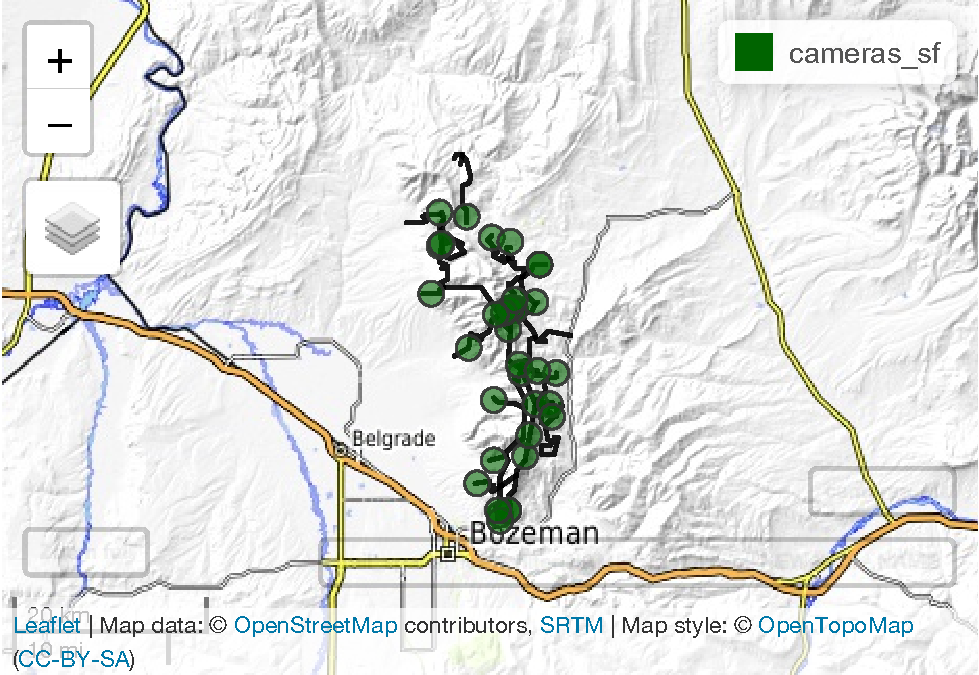
\includegraphics{Statistical-Analysis--Prediction-of-Trail-Use-in-Bridger-Mountains_files/figure-latex/location-test-1.pdf}
\caption{\label{fig:location-test}Interactive map of Bridger Mountain trails and camera counter locations. Available only in HTML format.}
\end{figure}

In Figures \autoref{fig:counter-byid-high} and
\ref{fig:counter-byid-low} we have time series plots for daily trail
use counts separated by trail subsections (fill color indicates trail
name). Most trail subsections have a single camera deployed, however a
subset (Baldy to Bridger, Ross Pass to Sacagawea Peak, Sacagawea Pass,
and Corbly Gulch) have two cameras. For subsections with multiple
cameras we have plotted the maximum count of trail uses between each
camera per day. Several counters are placed in subsequent subsections
along a single trail resulting in the capture of similar (i.e.
non-independent) trail use information. For example, counter IDs 4, 5,
6, 7, and 9 are all located on Bridger Ridge and while the total counts
for each counters are different (see Table \ref{tab:counter-summary})
the time series plots show very similar patterns of use of time
indicating non-independent counts.

\begin{figure}

{\centering 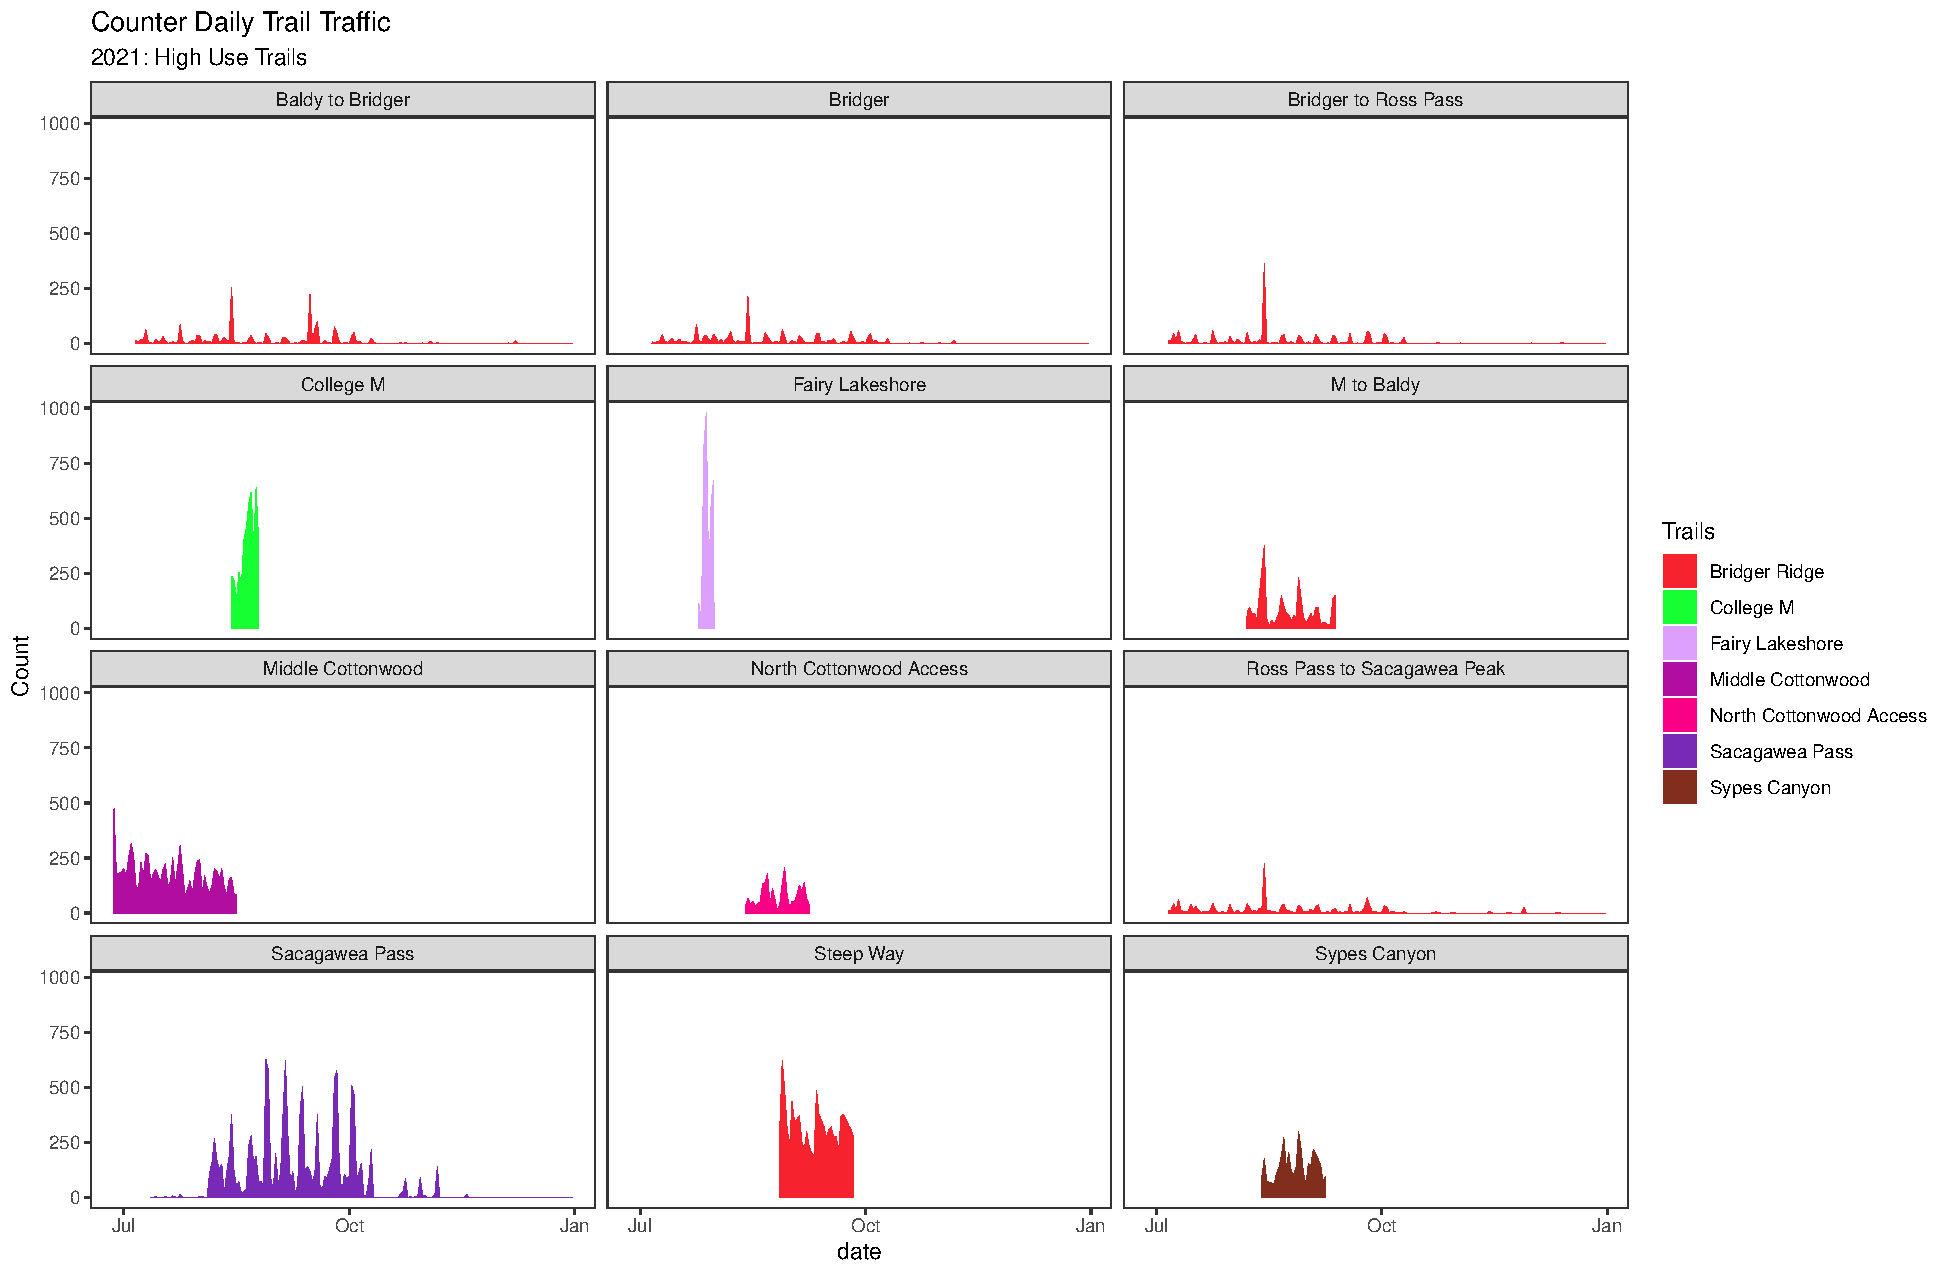
\includegraphics[width=1\linewidth]{../figures/Counter_bySubSection_TS_highuse} 

}

\caption{Timeseries plots of daily trail camera counts over time in the Bridger Mountains along high use trails. The following trails are not included in the analysis: Bridger, Bridger to Ross Pass, Fairy Lakeshore, M to Baldy, Ross Pass to Sacagawea Peak.}\label{fig:counter-byid-high}
\end{figure}

\begin{figure}

{\centering 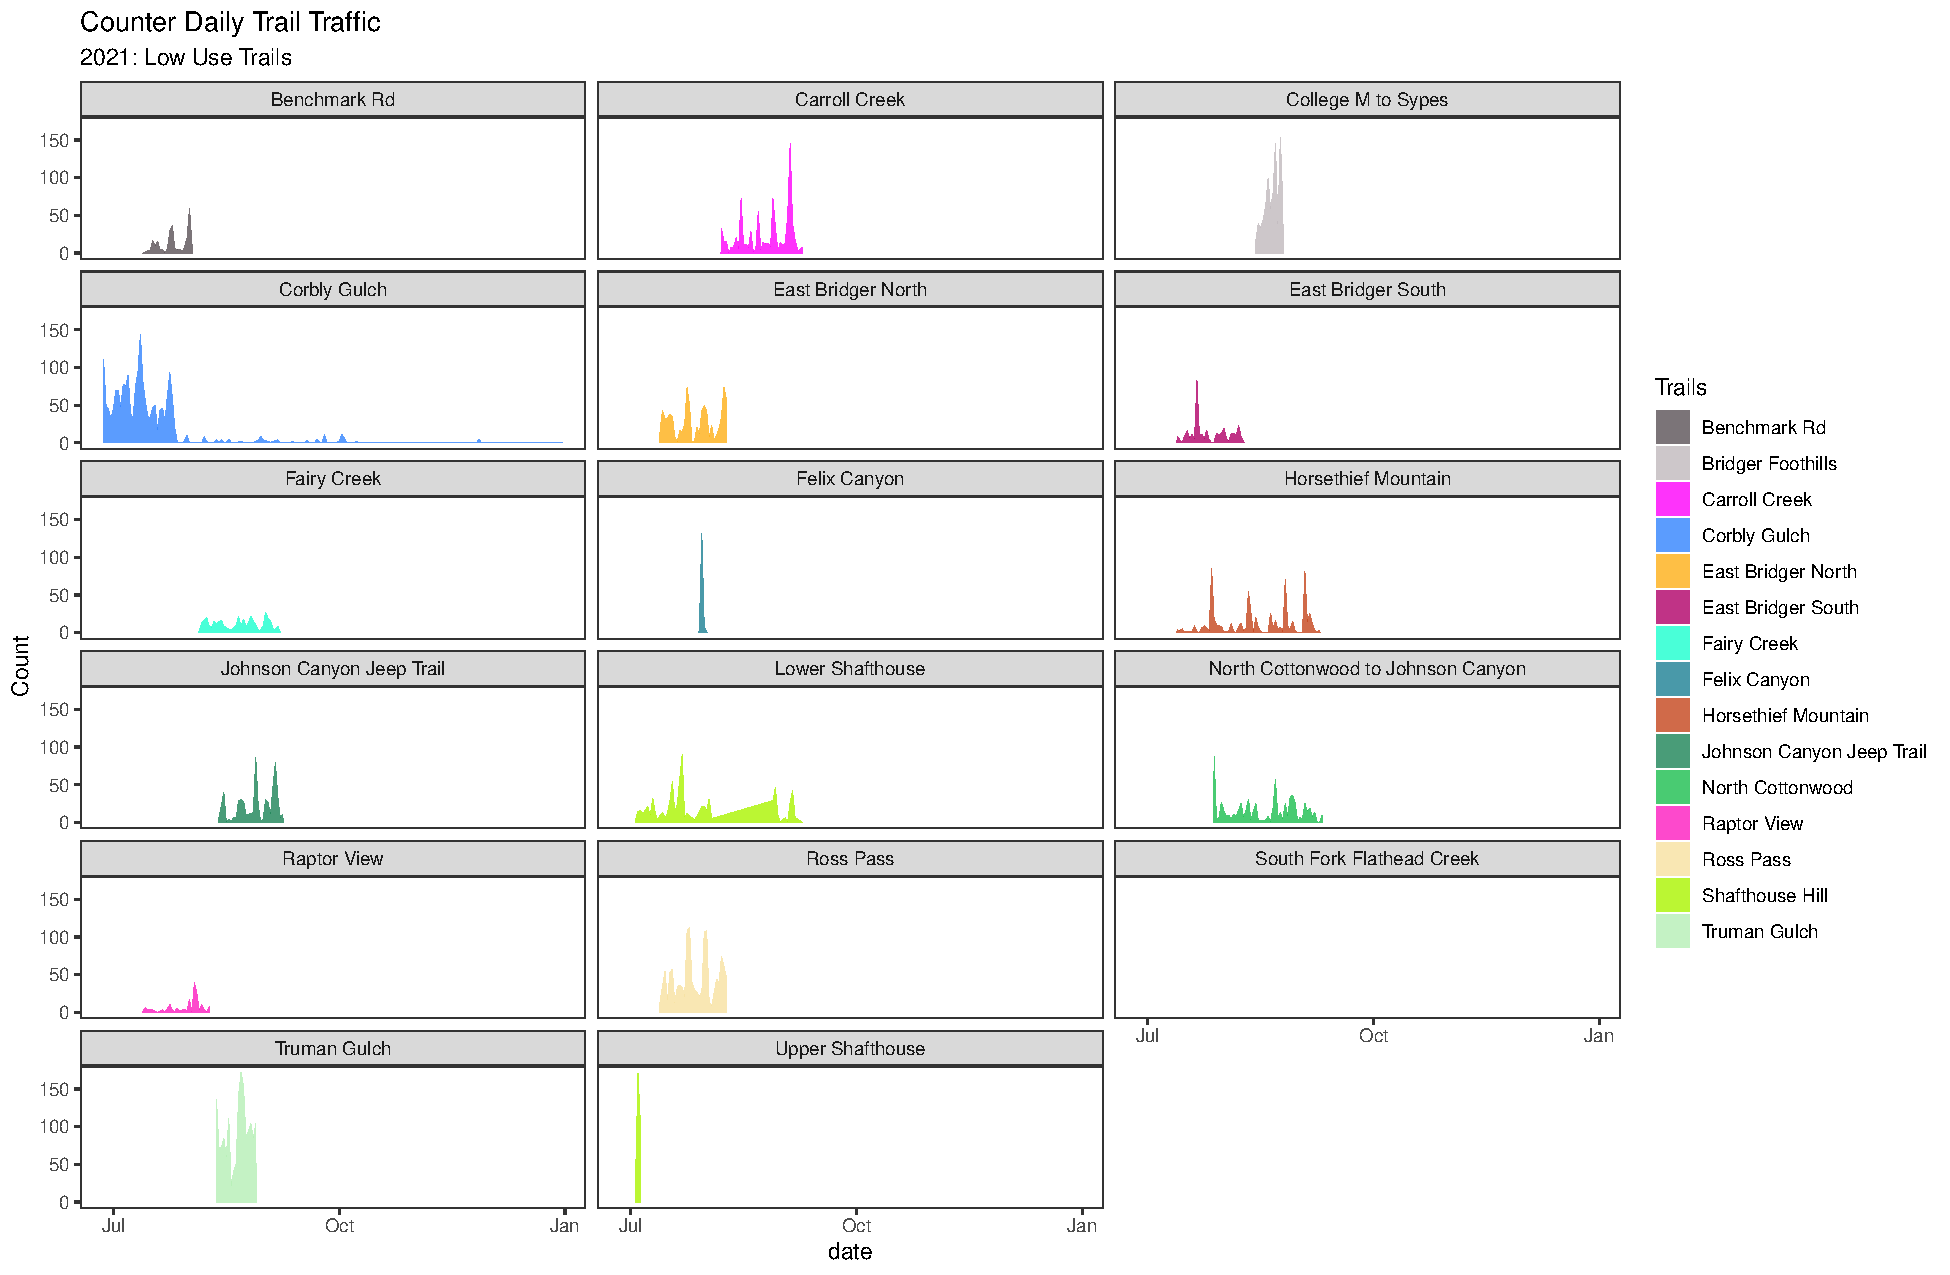
\includegraphics[width=1\linewidth]{../figures/Counter_bySubsection_TS_lowuse} 

}

\caption{Timeseries plots of daily trail camera counts over time in the Bridger Mountains along low use trails. The following trails are not included in the analysis: Felix Canyon, South Fork Flathead Creek.}\label{fig:counter-byid-low}
\end{figure}

In Table \ref{tab:counter-summary} we provide a summary of trail use
recorded for each counter deployed along trails in the Bridger
Mountains. In addition to total counts for each counter, the deployment
dates and duration of each trail counter camera (as determined by the
first and last date of data provided) and average daily trail use over
this deployment duration is reported.

\begin{landscape}\begin{table}

\caption{\label{tab:counter-summary}Total Number of Trail Camera Counts (2021)}
\centering
\begin{tabular}[t]{rl>{\raggedright\arraybackslash}p{4cm}rlll>{\raggedleft\arraybackslash}p{4cm}l}
\toprule
ID & Trail & Subsection & Count & Start & End & Deployment & Mean Count Per Day & Included in Analysis\\
\midrule
1 & Fairy Lakeshore & Fairy Lakeshore & 3412 & 07-25 & 07-31 & 7 days & 487.43 & No\\
2 & Fairy Creek & Fairy Creek & 376 & 08-05 & 09-07 & 34 days & 11.06 & Yes\\
3 & College M & College M & 4493 & 08-14 & 08-25 & 12 days & 374.42 & Yes\\
4 & Bridger Ridge & Baldy to Bridger & 1261 & 07-06 & 12-31 & 179 days & 7.04 & Yes\\
5 & Bridger Ridge & Baldy to Bridger & 1844 & 07-06 & 12-31 & 179 days & 10.30 & Yes\\
\addlinespace
6 & Bridger Ridge & Bridger & 1689 & 07-06 & 12-31 & 179 days & 9.44 & No\\
7 & Bridger Ridge & Bridger to Ross Pass & 1582 & 07-06 & 12-31 & 179 days & 8.84 & No\\
8 & Bridger Ridge & M to Baldy & 2635 & 08-07 & 09-12 & 37 days & 71.22 & No\\
9 & Bridger Ridge & Ross Pass to Sacagawea Peak & 1508 & 07-06 & 12-31 & 179 days & 8.42 & No\\
10 & Bridger Ridge & Ross Pass to Sacagawea Peak & 310 & 07-12 & 12-31 & 173 days & 1.79 & No\\
\addlinespace
11 & Bridger Ridge & Steep Way & 10122 & 08-27 & 09-26 & 31 days & 326.52 & Yes\\
12 & Sacagawea Pass & Sacagawea Pass & 5192 & 08-05 & 09-09 & 36 days & 144.22 & Yes\\
13 & Sacagawea Pass & Sacagawea Pass & 9485 & 07-12 & 12-31 & 173 days & 54.83 & Yes\\
14 & Horsethief Mountain & Horsethief Mountain & 628 & 07-13 & 09-09 & 59 days & 10.64 & Yes\\
15 & Carroll Creek & Carroll Creek & 757 & 08-07 & 09-09 & 34 days & 22.26 & Yes\\
\addlinespace
16 & Felix Canyon & Felix Canyon & 146 & 07-29 & 08-01 & 4 days & 36.50 & No\\
17 & Raptor View & Raptor View & 158 & 07-13 & 08-09 & 28 days & 5.64 & Yes\\
18 & Sypes Canyon & Sypes Canyon & 3868 & 08-13 & 09-08 & 27 days & 143.26 & Yes\\
19 & Bridger Foothills & College M to Sypes & 834 & 08-14 & 08-25 & 12 days & 69.50 & Yes\\
20 & Truman Gulch & Truman Gulch & 1585 & 08-12 & 08-28 & 17 days & 93.24 & Yes\\
\addlinespace
21 & East Bridger South & East Bridger South & 321 & 07-13 & 08-09 & 28 days & 11.46 & Yes\\
22 & East Bridger North & East Bridger North & 780 & 07-13 & 08-09 & 28 days & 27.86 & Yes\\
23 & Shafthouse Hill & Lower Shafthouse & 687 & 07-03 & 09-09 & 69 days & 9.96 & Yes\\
24 & Shafthouse Hill & Upper Shafthouse & 303 & 07-03 & 07-05 & 3 days & 101.00 & No\\
25 & South Fork Flathead Creek & South Fork Flathead Creek & 91 & 07-03 & 07-03 & 1 days & 91.00 & No\\
\addlinespace
26 & Corbly Gulch & Corbly Gulch & 1766 & 06-27 & 07-26 & 30 days & 58.87 & Yes\\
27 & Corbly Gulch & Corbly Gulch & 165 & 07-13 & 12-31 & 172 days & 0.96 & Yes\\
28 & North Cottonwood & North Cottonwood to Johnson Canyon & 662 & 07-28 & 09-10 & 45 days & 14.71 & Yes\\
29 & North Cottonwood Access & North Cottonwood Access & 2124 & 08-13 & 09-08 & 27 days & 78.67 & Yes\\
30 & Ross Pass & Ross Pass & 1246 & 07-13 & 08-09 & 28 days & 44.50 & Yes\\
\addlinespace
31 & Middle Cottonwood & Middle Cottonwood & 9060 & 06-27 & 08-16 & 51 days & 177.65 & Yes\\
32 & Johnson Canyon Jeep Trail & Johnson Canyon Jeep Trail & 573 & 08-13 & 09-08 & 27 days & 21.22 & Yes\\
33 & Benchmark Rd & Benchmark Rd & 244 & 07-13 & 08-02 & 21 days & 11.62 & Yes\\
\bottomrule
\end{tabular}
\end{table}
\end{landscape}

Due to low deployment times and possibly unreliable camera recordings,
the following trails (numbers refer to counter IDs) are removed from
this analysis:

\begin{itemize}
\tightlist
\item
  \#1 - Fairy Lakeshore
\item
  \#16 - Felix Canyon
\item
  \#24 - Shafthouse Hill (Upper Shafthouse)
\item
  \#25 - South Fork Flathead Creek.
\end{itemize}

\hypertarget{hourly-data}{%
\subsubsection{Hourly Data}\label{hourly-data}}

For each trail counter camera deployed data is provided on a daily
scale. Finer resolution data (i.e.~hourly counts rather than daily) are
available for 17 trails. Figures \ref{fig:hourly-high} and
\ref{fig:hourly-low} shows trail use patterns with use hitting highest
counts on the weekends, as expected.

The most likely use for these days is a quick look at how daily activity
trends look (i.e.~are there more hikers in mornings vs afternoon?).
However since Strava data is not available at this resolution, it would
not be easy to model this trend without a lot of data (i.e.~counters
deployed for longer amounts of time) to provide information on this
trend in any model used.

\begin{figure}

{\centering 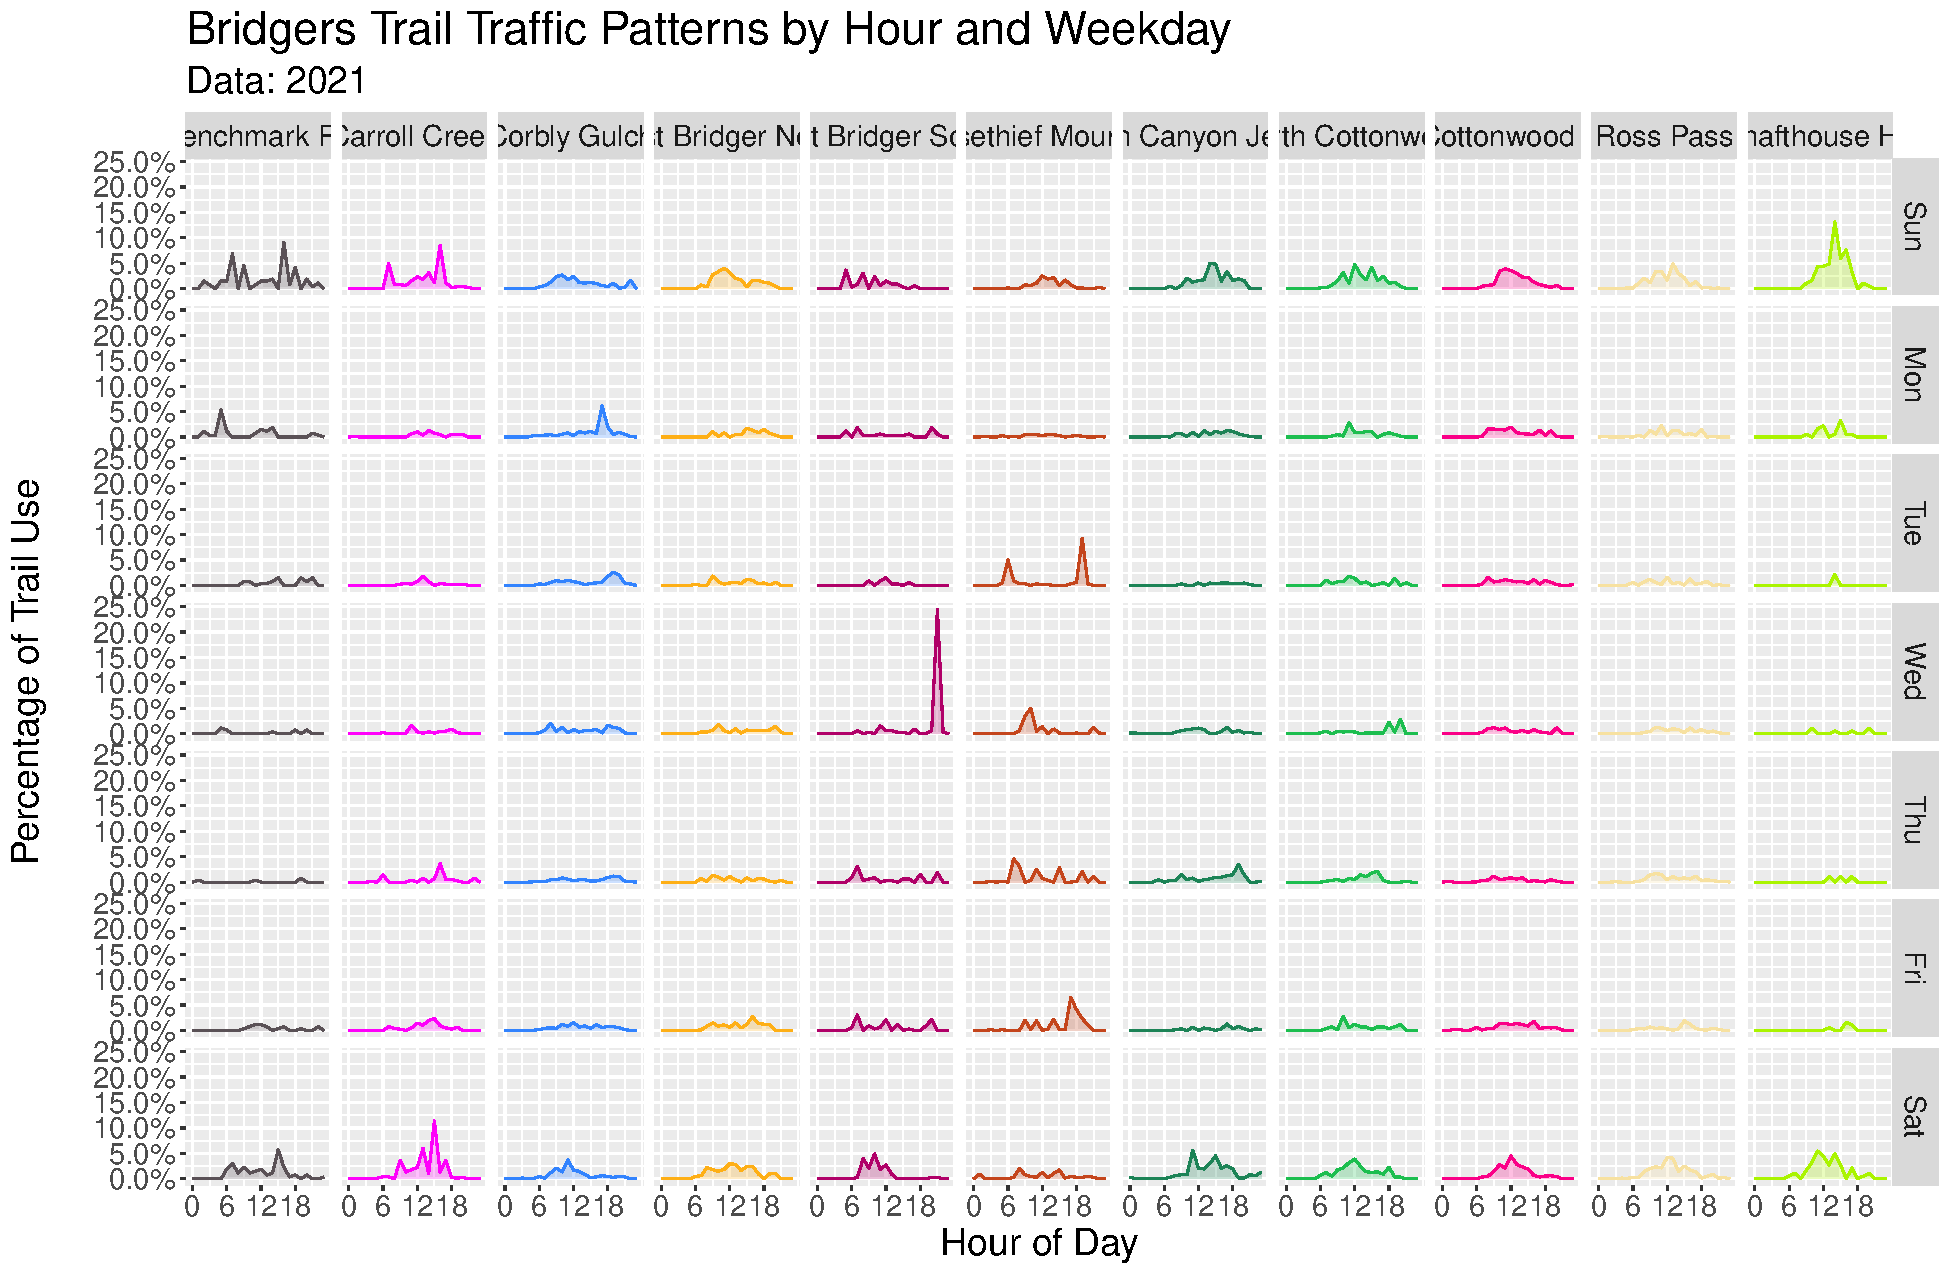
\includegraphics[width=1\linewidth]{../figures/hourly_bydayofweek_highuse} 

}

\caption{Bridger Mountain trail traffic patterns by hour and day of week.}\label{fig:hourly-high}
\end{figure}

\begin{figure}

{\centering 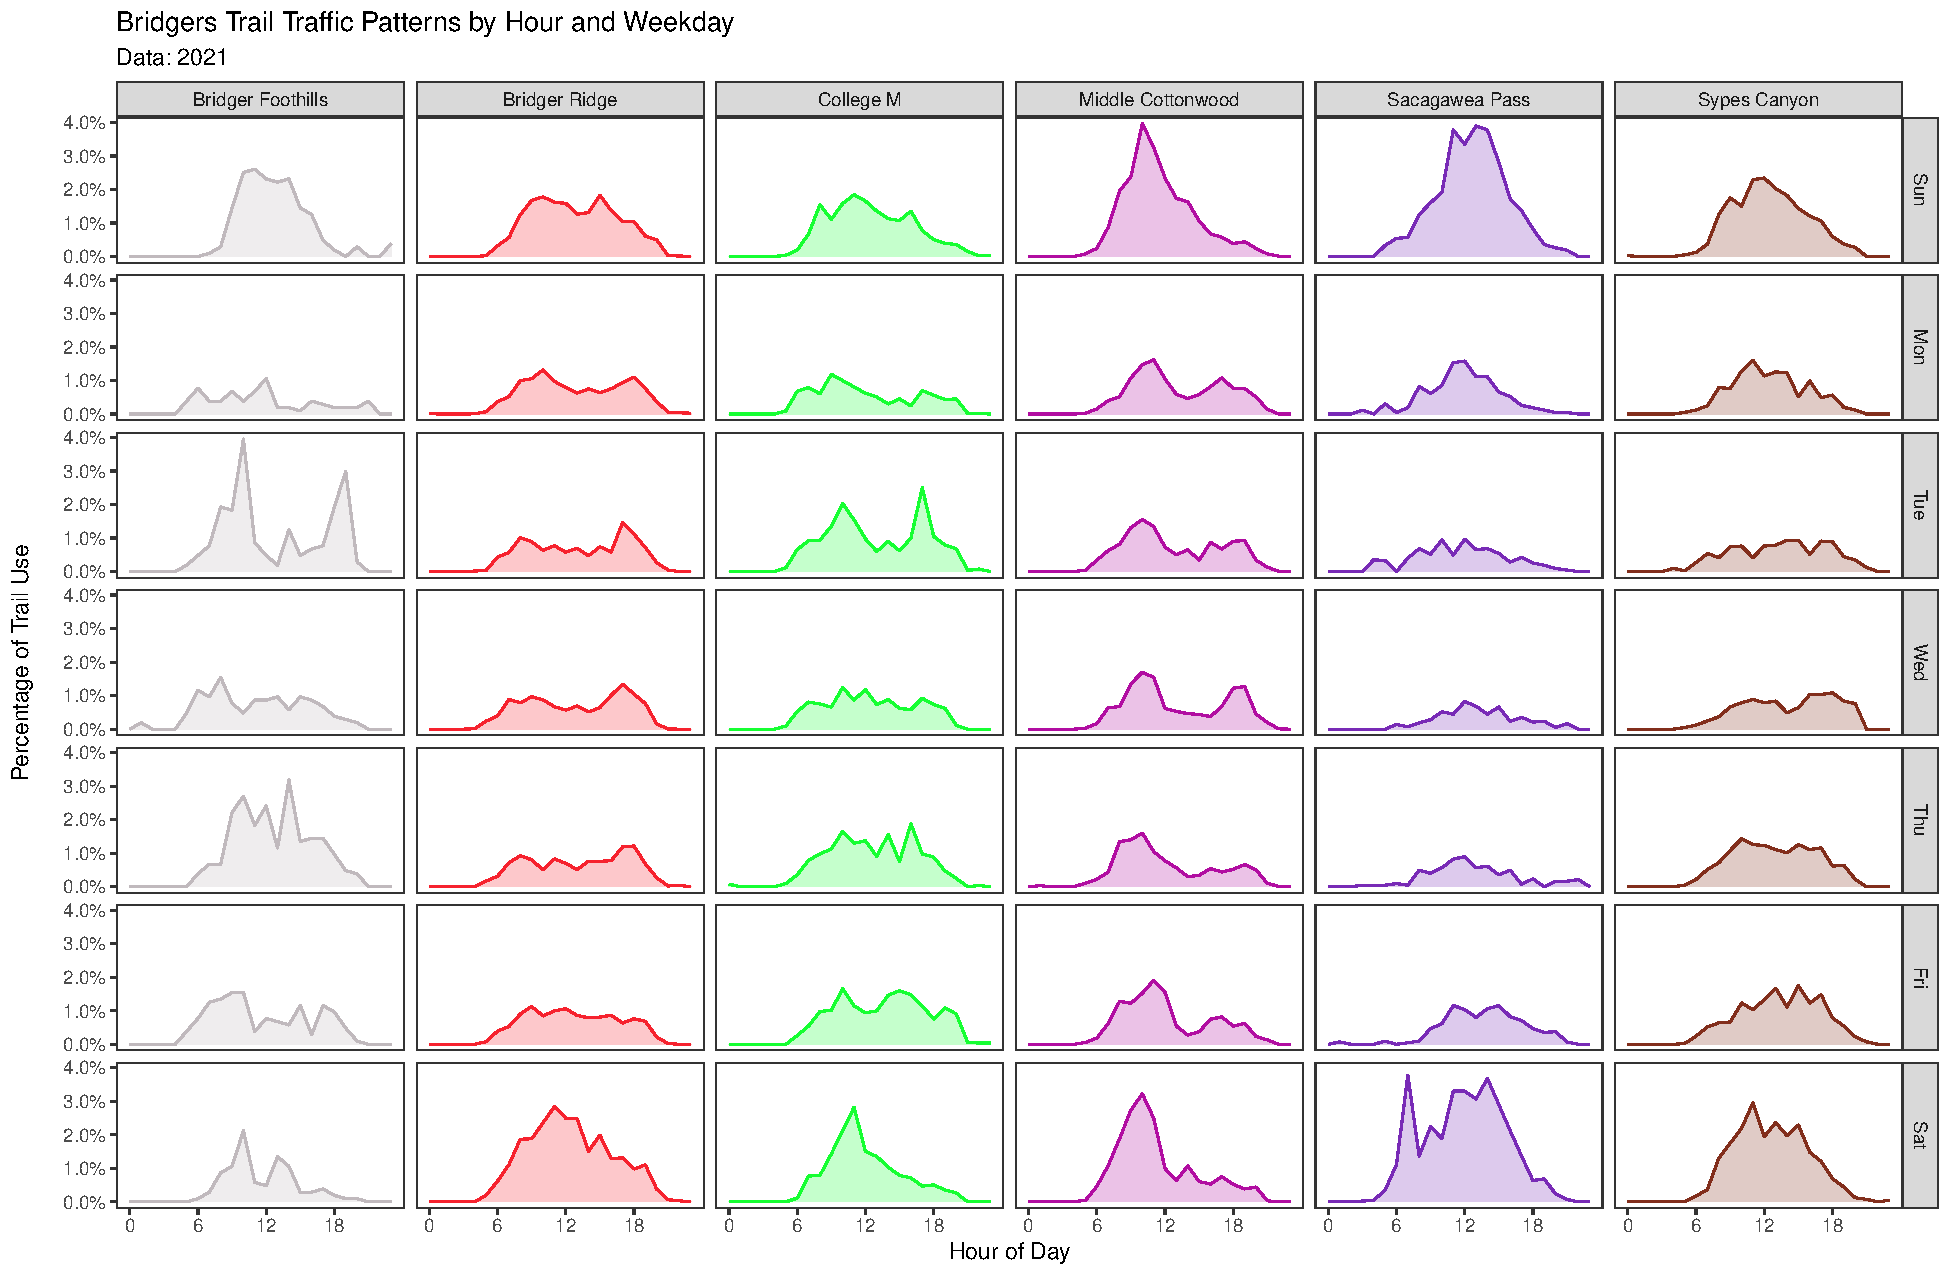
\includegraphics[width=1\linewidth]{../figures/hourly_bydayofweek_lowuse} 

}

\caption{Bridger Mountain trail traffic patterns by hour and day of week.}\label{fig:hourly-low}
\end{figure}

\hypertarget{strava-data}{%
\subsubsection{Strava Data}\label{strava-data}}

Strava count data are made available through Strava Metro. Data are
binned (intervals of 5 with ceiling rounding) and aggregated on multiple
scales (daily, monthly, annual). Counts are available as ``total trips''
and ``total people''. Total trips should always be larger than the total
people count as people sometimes make multiple passes of a single trail
(e.g.~M laps). Strava trails are subdivided into ``edges''. Edge IDs (for
the counter locations which often aligns with the trailhead edge) are
available in the Counter data. Strava count data are available for the
entire year of 2021 (not just summer monitoring as in the counter data).
These data also include the overarching trail name and number (e.g.
511 - Bridger Foothills) that also correspond to the counter data
provided by HE.

It is important to note that when considering Strava data at the Trail
scale (rather than edge scale) you are propagating rounding errors for
each segment forward (+\_ 1-4 for each edge?). Similarly, aggregating
the data in the daily data frame to a monthly timescale will likely not
match the information provided in the monthly data frame.

Table \ref{tab:strava-summary} provides a summary of Strava data for
the entire year. For each trail, the aggregated annual trail use count
is provided as well as the number of Strava defined edges.

\begin{table}

\caption{\label{tab:strava-summary}Total Number of Strava Counts (2021)}
\centering
\begin{tabular}[t]{lrrrl}
\toprule
trailname & count & edges & Mean Count per Day & Included in Analysis\\
\midrule
Benchmark Road & 50 & 8 & 0.14 & No\\
Bridger Foothills & 61185 & 30 & 167.63 & Yes\\
Bridger Ridge & 56395 & 40 & 154.51 & Yes\\
Carrol Creek & 625 & 10 & 1.71 & No\\
College M & 27420 & 4 & 75.12 & Yes\\
\addlinespace
Corbly Gulch & 12010 & 13 & 32.90 & Yes\\
E Bridger North & 4150 & 15 & 11.37 & No\\
E Bridger South & 70 & 4 & 0.19 & No\\
Fairy Creek & 2130 & 16 & 5.84 & Yes\\
Fairy Lake & 15 & 1 & 0.04 & No\\
\addlinespace
Fairy Lake Shortcut & 305 & 1 & 0.84 & No\\
Fairy Lakeshore & 640 & 4 & 1.75 & No\\
Felix Canyon Rd & 885 & 7 & 2.42 & No\\
Felix Canyon Trail & 50 & 2 & 0.14 & No\\
Flathead Pass Rd & 755 & 18 & 2.07 & No\\
\addlinespace
Horsethief Mountain & 30 & 3 & 0.08 & Yes\\
Johnson Canyon Jeep Trail & 160 & 11 & 0.44 & Yes\\
M shortcut & 5700 & 3 & 15.62 & No\\
Middle Cottonwood & 16135 & 8 & 44.21 & Yes\\
New World Gulch & 2140 & 6 & 5.86 & No\\
\addlinespace
North Cottonwood & 4170 & 16 & 11.42 & Yes\\
North Cottonwood Access & 2525 & 4 & 6.92 & Yes\\
Raptor View & 570 & 4 & 1.56 & Yes\\
Ross Pass & 1600 & 4 & 4.38 & Yes\\
S Fork Brackett Creek & 280 & 3 & 0.77 & No\\
\addlinespace
S Fork Flathead Creek & 5 & 1 & 0.01 & No\\
Sacagawea Pass & 2350 & 2 & 6.44 & Yes\\
Shafthouse Hill & 1640 & 9 & 4.49 & Yes\\
Sypes Canyon & 25575 & 11 & 70.07 & Yes\\
Truman Gulch & 7185 & 6 & 19.68 & Yes\\
\addlinespace
Upper Brackett Creek & 430 & 6 & 1.18 & No\\
\bottomrule
\end{tabular}
\end{table}

Figures \ref{fig:strava-bytrailname-high} and
\ref{fig:strava-bytrailname-low} show time series plots for daily trail
use counts (maximum number of trips over all edges in a trail) separated
by trail (fill color indicates trail name).

\begin{figure}

{\centering 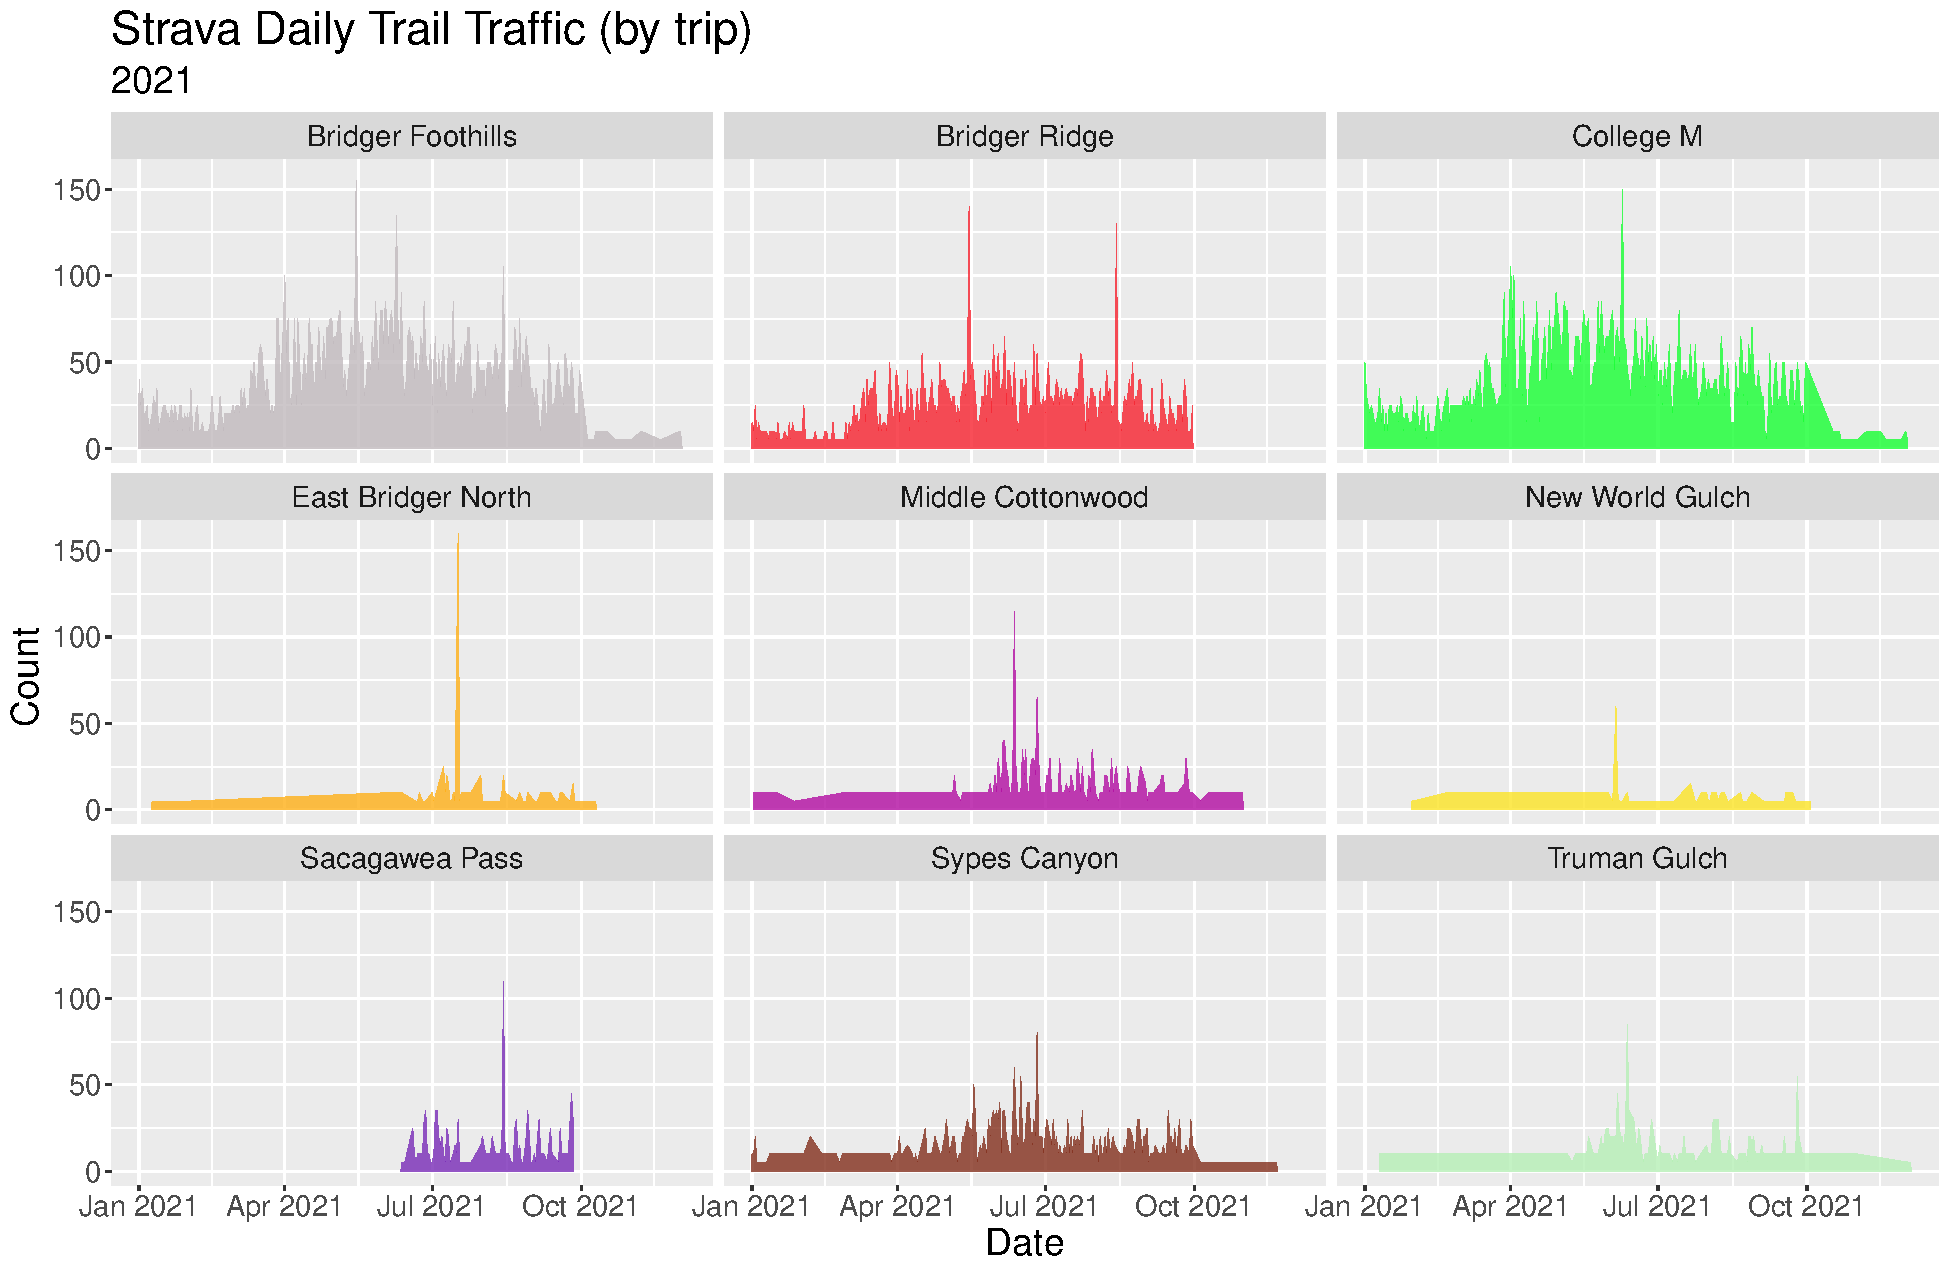
\includegraphics[width=1\linewidth]{../figures/Strava_day_TS_bytrip_high} 

}

\caption{Timeseries plots of daily Strava trip counts over time in the Bridger Mountains along high use trails. The following trails are not included in the analysis: New World Gulch.}\label{fig:strava-bytrailname-high}
\end{figure}

\begin{figure}

{\centering 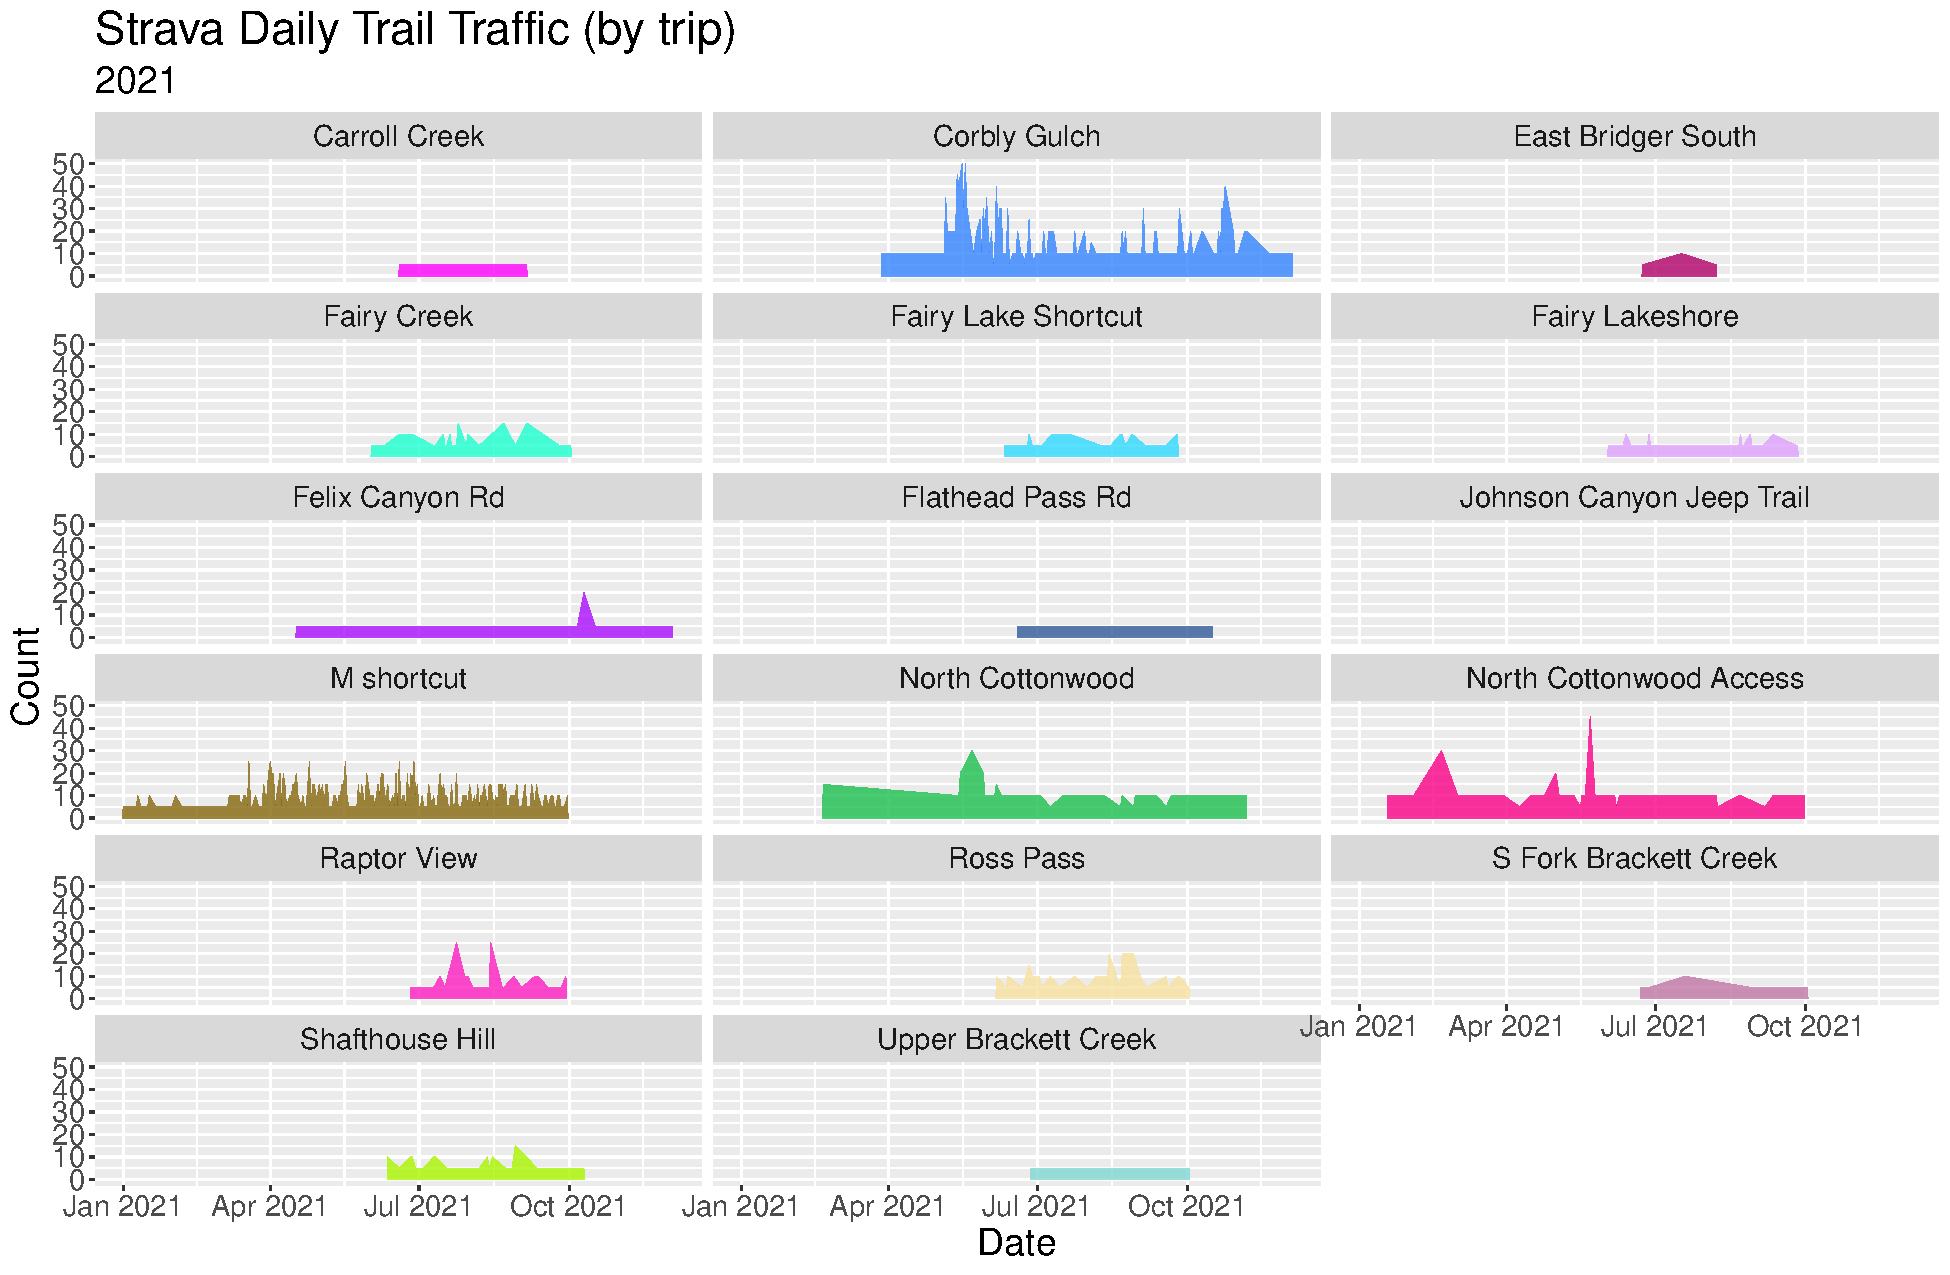
\includegraphics[width=1\linewidth]{../figures/Strava_day_TS_bytrip_low} 

}

\caption{Timeseries plots of daily Strava trip counts over time in the Bridger Mountains along high use trails. The following trails are not included in the analysis: Fairy Lake Shortcut, Fairy Lakeshore, Felix Canyon Rd, M Shortcut, S Fork Brackett Creek.}\label{fig:strava-bytrailname-low}
\end{figure}

\hypertarget{ATData}{%
\subsubsection{AllTrails Data}\label{ATData}}

AllTrails has provided number of daily searchs for each trail for
2020-2022. A seven day preceding moving average number of search terms
was calculated for each trail. Figures
\ref{fig:alltrails-bytrailname-high} and
\ref{fig:alltrails-bytrailname-low} show time series plots for daily
trail searches (7-day moving average) separated by trail (fill color
indicates trail name).

\begin{figure}

{\centering 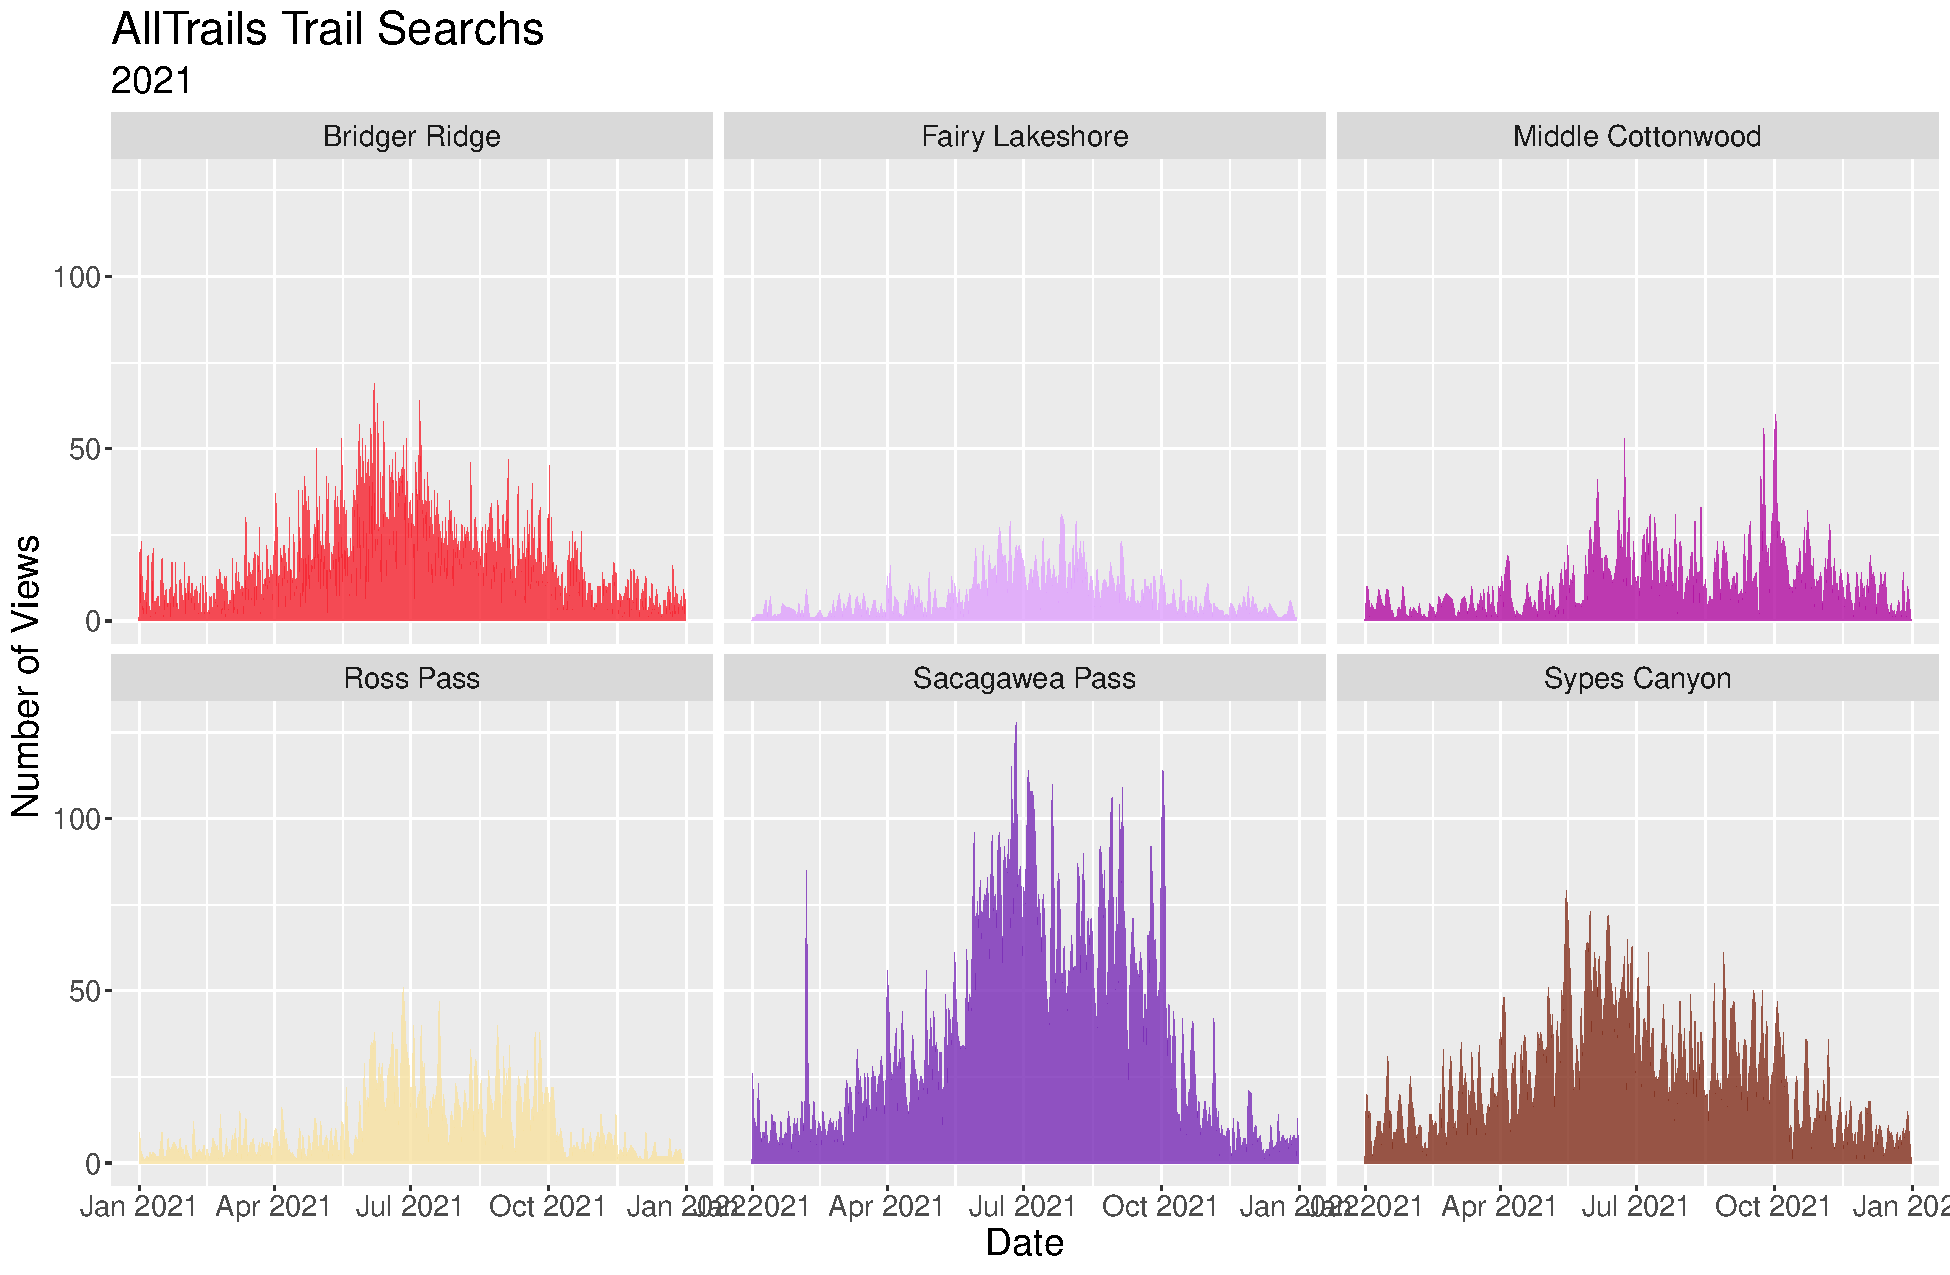
\includegraphics[width=1\linewidth]{../figures/allTrails_search_TS_high} 

}

\caption{Timeseries plots of daily AllTrails trail searches as a moving average over time in the Bridger Mountains along high use trails.}\label{fig:alltrails-bytrailname-high}
\end{figure}

\begin{figure}

{\centering 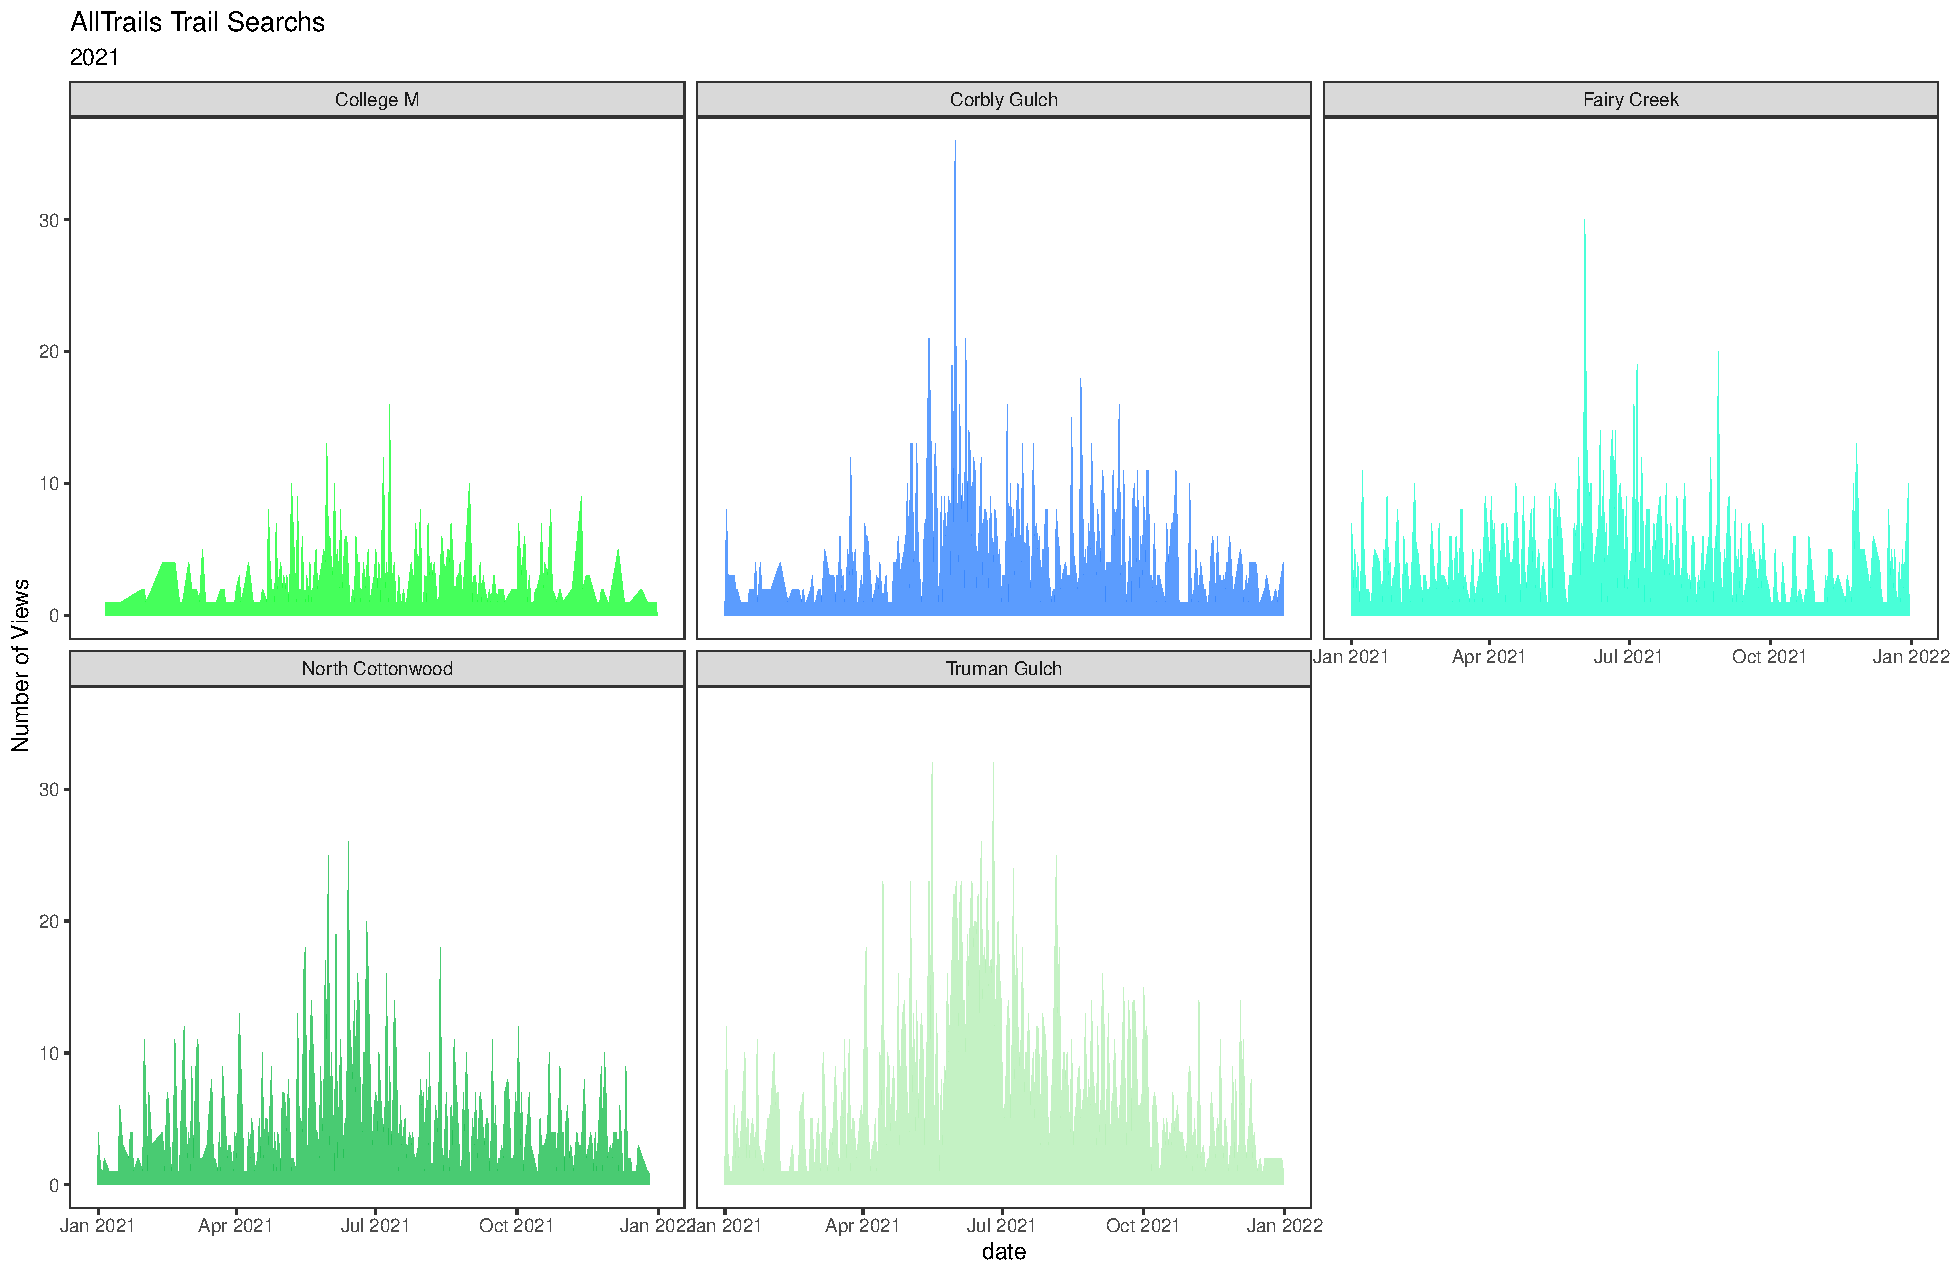
\includegraphics[width=1\linewidth]{../figures/allTrails_search_TS_low} 

}

\caption{Timeseries plots of daily AllTrails trail searches as a moving average over time in the Bridger Mountains along low use trails.}\label{fig:alltrails-bytrailname-low}
\end{figure}

\hypertarget{weather-covariates}{%
\subsection{Weather Covariates}\label{weather-covariates}}

The following weather covariates are available on a daily basis:

\begin{enumerate}
\def\labelenumi{\arabic{enumi}.}
\tightlist
\item
  Precipitation (in.)
\item
  Temperature Max (degrees Fahrenheit)
\item
  Temperature Min (degrees Fahrenheit)
\item
  Mean Air Quality (AQI)
\item
  Mean PM\_25 Concentration (micrograms per cubic meter)
\end{enumerate}

These data do not vary spatially only temporally (i.e.~the resolution is
not fine enough to parse out different weather between trails on a given
day). Figure \ref{fig:covariate-plots} shows each covariate over time
for 2021. Clear collinearity between several covariates (e.g.~Min and
Max Air Temperature) is apparent, and is considered when selecting
covariates for inclusion in analysis.

\begin{figure}

{\centering 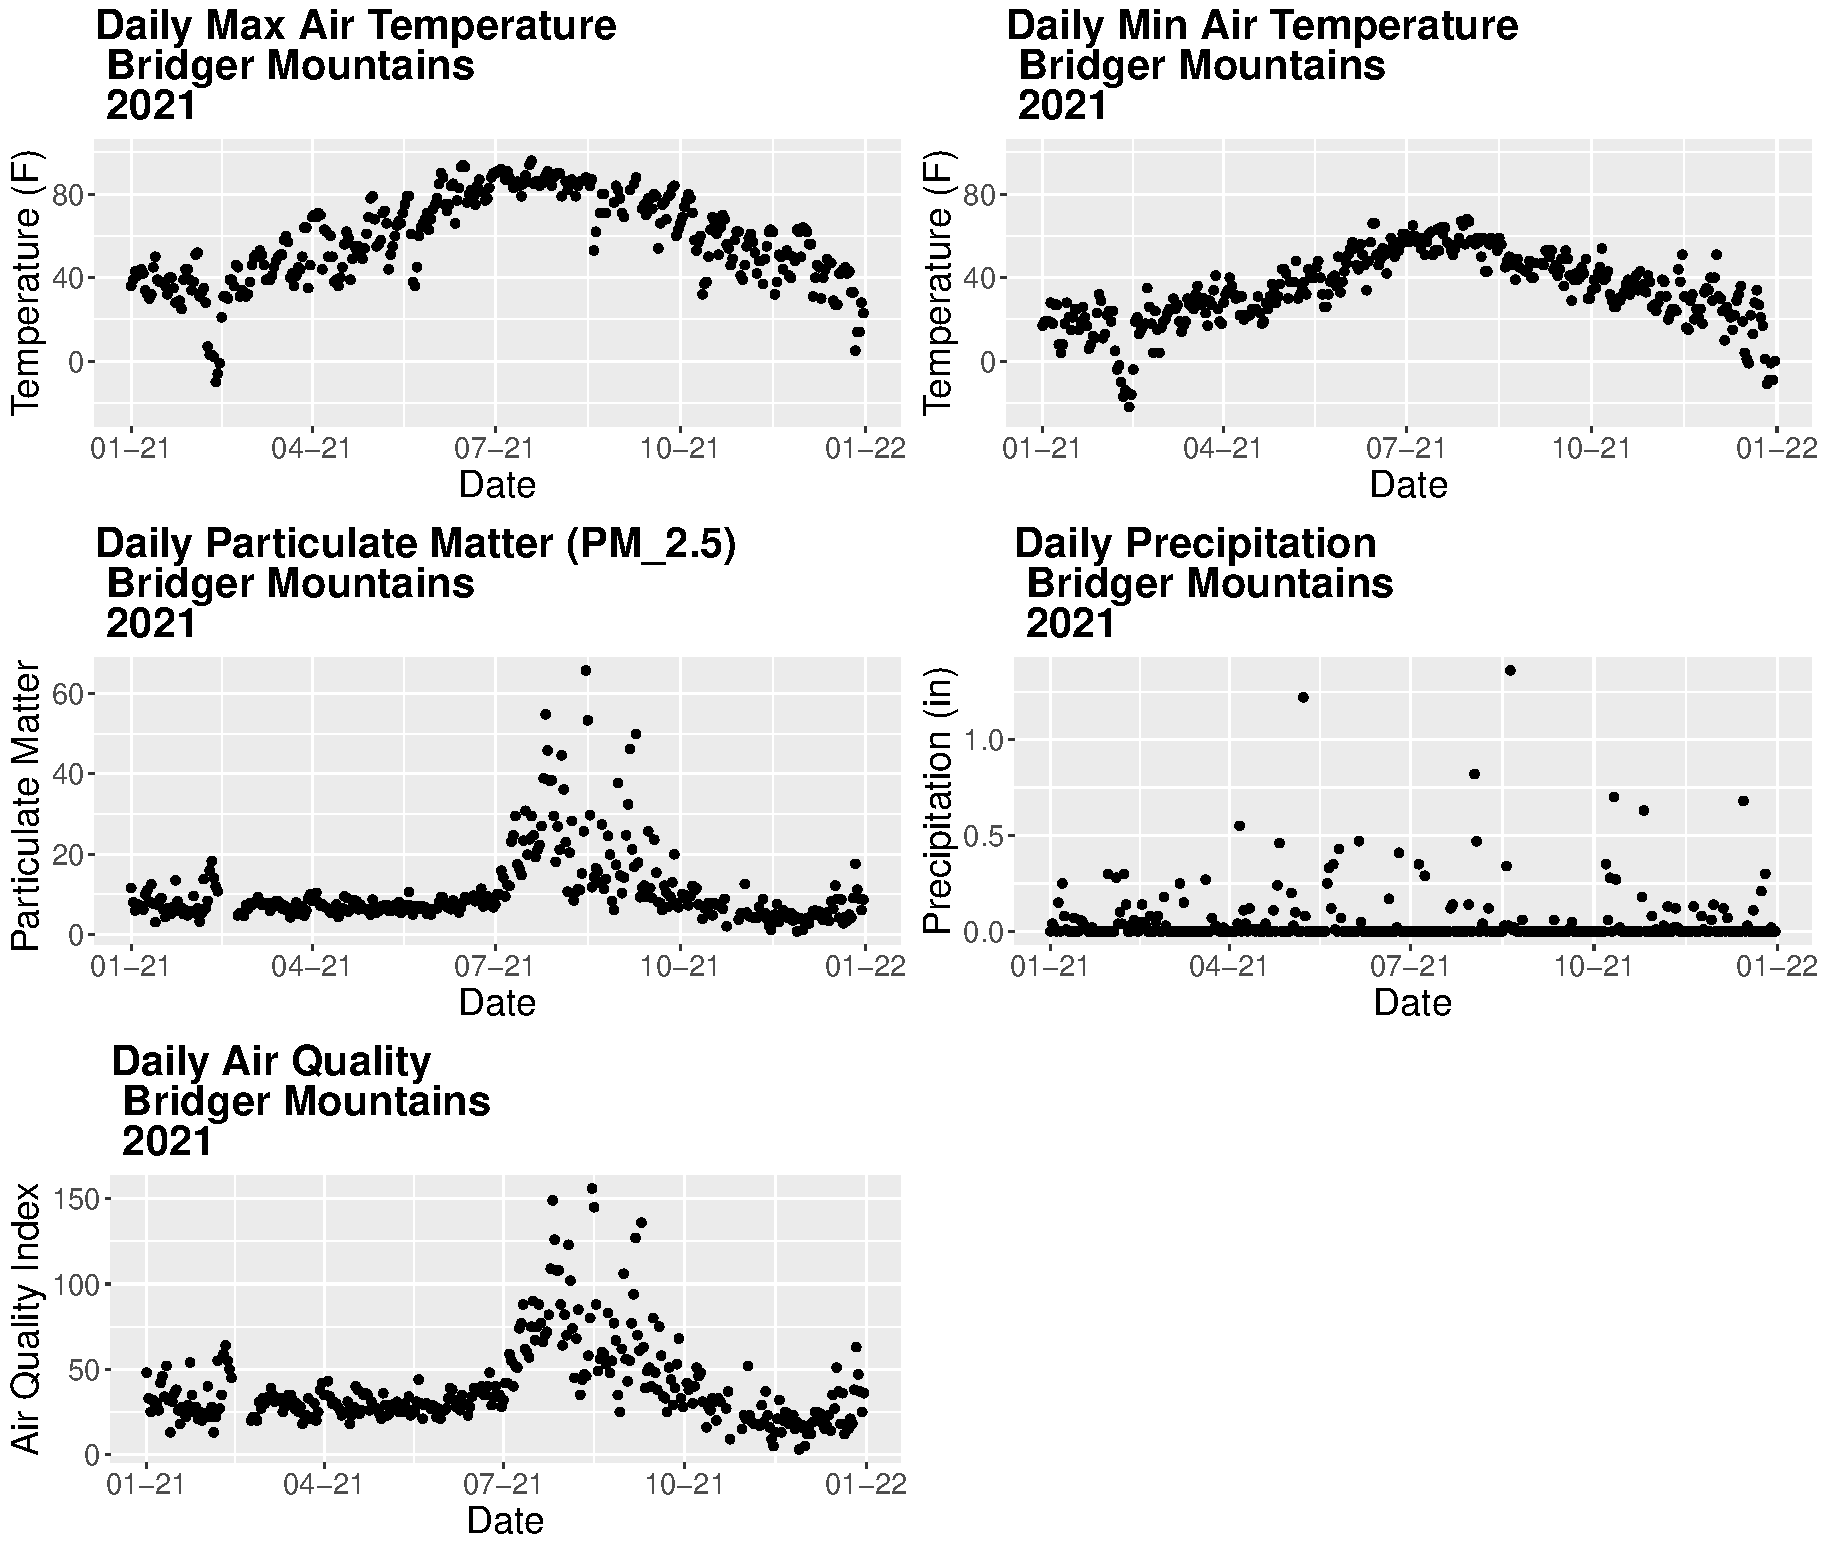
\includegraphics[width=1\linewidth]{../figures/weatherplots} 

}

\caption{Weather covariate values over time.}\label{fig:covariate-plots}
\end{figure}

\hypertarget{trail-characteristics}{%
\subsection{Trail Characteristics}\label{trail-characteristics}}

The following characteristics are provided at the trail level.

\begin{itemize}
\tightlist
\item
  Latitude/Longitude (of trailhead and camera location)
\item
  Time/Distance from Bozeman, MT
\item
  Parking lot size (as three-level factor)
\item
  Description/Class (4-level factor of development)
\item
  Motorized vehicle use (3-level factor)
\item
  Indicators for use of the following:

  \begin{itemize}
  \tightlist
  \item
    Dirt bikes
  \item
    ATVS
  \item
    Hiking
  \item
    Pack/Saddle
  \item
    Bicycle
  \end{itemize}
\end{itemize}

Table \ref{tab:table-char} provides an overview of these summaries.

\begin{landscape}\begin{table}

\caption{\label{tab:table-char}Bridger Mountain Trail Characteristics (2021)}
\centering
\begin{tabular}[t]{lllllr}
\toprule
Name & Subsection & Lot Size & Developed & Moterized Vehicle Use & Drive Time (mins)\\
\midrule
Fairy Lakeshore & Fairy Lakeshore & L & Moderately Developed & Non-Motorized & 57.16\\
Fairy Creek & Fairy Creek & L & Developed & Wheeled OHV 50" or < & 46.39\\
Fairy Lake & Fairy Lake & L & Moderately Developed & Non-Motorized & 57.16\\
College M & College M & L & Highly Developed & Non-Motorized & 12.16\\
Bridger Ridge & Baldy to Bridger & L & Minimally Developed & Non-Motorized & 12.16\\
\addlinespace
Bridger Ridge & Bridger & L & Minimally Developed & Non-Motorized & 31.70\\
Bridger Ridge & Bridger to Ross Pass & S & Minimally Developed & Non-Motorized & 41.00\\
Bridger Ridge & M to Baldy & L & Minimally Developed & Non-Motorized & 12.16\\
Bridger Ridge & Ross Pass to Sacagawea Peak & L & Minimally Developed & Non-Motorized & 41.00\\
Bridger Ridge & Sacagawea Peak to Sacagawea Pass & L & Minimally Developed & Non-Motorized & 57.16\\
\addlinespace
Bridger Ridge & Steep Way & L & Moderately Developed & Non-Motorized & 12.16\\
Sacagawea Pass & Sacagawea Pass & L & Developed & Non-Motorized & 57.16\\
Horsethief Mountain & Horsethief Mountain & S & Developed & Non-Motorized & 78.00\\
Carroll Creek & Carroll Creek & L & Highly Developed & Wheeled OHV 50" or < & 46.39\\
Felix Canyon Trail & Felix Canyon Trail & S & Highly Developed & Wheeled OHV 50" or < & 43.56\\
\addlinespace
Raptor View & Raptor View & M & Developed & Non-Motorized & 31.70\\
Sypes Canyon & Sypes Canyon & M & Developed & Non-Motorized & 14.45\\
Bridger Foothills & Bostwick to Truman & L & Minimally Developed & Non-Motorized & 25.74\\
Bridger Foothills & College M & L & Developed & Non-Motorized & 12.16\\
Bridger Foothills & College M to Sypes & L & Developed & Non-Motorized & 12.16\\
\addlinespace
Bridger Foothills & Jones to Ross Pass & S & Minimally Developed & Non-Motorized & 41.00\\
Bridger Foothills & Middle Cottonwood to Bostwick & M & Developed & Non-Motorized & 17.78\\
Bridger Foothills & Ross Pass to Sacagawea Pass & S & Developed & Non-Motorized & 41.00\\
Bridger Foothills & Sypes to Middle Cottonwood & M & Developed & Non-Motorized & 14.45\\
Bridger Foothills & Truman to Jones & L & Minimally Developed & Non-Motorized & 25.74\\
\addlinespace
Truman Gulch & Truman Gulch & L & Developed & Dirt Bikes (seasonal) & 25.74\\
East Bridger South & East Bridger South & L & Highly Developed & Non-Motorized & 31.70\\
East Bridger North & East Bridger North & M & Developed & Non-Motorized & 27.41\\
Shafthouse Hill & Lower Shafthouse & M & Developed & Non-Motorized & 40.97\\
Shafthouse Hill & Upper Shafthouse & S & Developed & Non-Motorized & 54.34\\
\addlinespace
South Fork Flathead Creek & South Fork Flathead Creek & S & Highly Developed & Wheeled OHV 50" or < & 49.88\\
Corbly Gulch & Corbly Gulch & S & Developed & Dirt Bikes (seasonal) & 26.48\\
North Cottonwood & North Cottonwood to Johnson Canyon & L & Developed & Non-Motorized & 39.33\\
North Cottonwood & North Cottonwood to Ridge & M & Developed & Non-Motorized & 33.46\\
North Cottonwood Access & North Cottonwood Access & M & Developed & Non-Motorized & 33.46\\
\addlinespace
Ross Pass & Ross Pass & S & Developed & Dirt Bikes (seasonal) & 41.00\\
Middle Cottonwood & Middle Cottonwood & M & Highly Developed & Dirt Bikes (seasonal) & 17.78\\
Johnson Canyon Jeep Trail & Johnson Canyon Jeep Trail & L & Highly Developed & Wheeled OHV 50" or < & 39.33\\
Felix Canyon Rd & Felix Canyon Rd & L & Highly Developed & Wheeled OHV 50" or < & 43.56\\
Benchmark Rd & Benchmark Rd & S & Highly Developed & Wheeled OHV 50" or < & 47.75\\
\bottomrule
\end{tabular}
\end{table}
\end{landscape}

\hypertarget{Models}{%
\chapter{Explanation of Models}\label{Models}}

The aim of this project is to understand and predict the pattern of
trail use recorded at multiple multi-use trails in the Bridger
Mountains. We want to be able to predict trail use over a full calendar
year and in locations where no trail counter data exist, within the
Bridgers and nearby trails. Here, we provide a description of the
statistical approach employed (generalized additive mixture modeling) in
addition to brief overviews of modelling approaches that \texttt{gamm}s build
upon (e.g.~linear regression, generalized linear regression, and
generalized additive models). In Section \ref{MidCot}, we further this
exploration in model choice by applying each to a single trail, Middle
Cottonwood.

\hypertarget{linear-regression-model}{%
\section{Linear Regression Model}\label{linear-regression-model}}

Linear regression is used to model the linear relationship between a
scalar or vector response and one or more explanatory variables.

\[ 
 y_{i}=\beta_{0}+\beta_{1}x_{i,1}+\beta_{2}x_{i,2}+\ldots+\beta_{p-1}x_{i,p-1}+\epsilon_{i}. 
\]

where \(y_i\) is (are) the response variable(s) for each unit (\(i\)),
\(x_{i, p-1}\) are the explanatory variables, and \(\beta_{p-1}\) are the
parameter coefficients. The errors, \(\epsilon_i\), are assumed to be
normally distributed with mean 0 and constant variance \(\sigma^2\). In
this approach one would find estimates for the \(\beta_{p-1}\) parameters
using values that minimize the sum of squared errors for the sample.

\hypertarget{generalized-linear-regression-model}{%
\section{Generalized Linear Regression Model}\label{generalized-linear-regression-model}}

In generalized linear models, the response variable \(y_i\) is now assumed
to follow an exponential family distribution with mean \(\mu_i\), which is
assumed to be some (often nonlinear) function of \(x_i^T\beta\). Note that
the covariates affect the distribution of \(y_i\) only through the linear
combination \(x_i^T\beta\).

The general form, written now in matrix multiplication format, is: \[
\begin{gathered}
g(\mu)=\eta=X \beta \\
E(y)=\mu=g^{-1}(\eta)
\end{gathered}
\] where \(g(.)\) is a link function relating the mean \(\mu\) to the linear
predictor(s) \(X \beta\) (also denoted by \(\eta\)). Recall in linear
regression we assume a Gaussian (i.e.~normal) distribution for the
response, we assume equal variance for all observations, and that there
is a direct link of the linear predictor and the expected value \(\mu\),
i.e.~\(\mu = X\beta\). As such, the typical linear regression model is a
generalized linear model with a Gaussian distribution and `identity'
link function.

For count data, a Poisson distribution is used. There is only one
parameter to be considered, \(\lambda\), since for the Poisson the mean
and variance are equal. For the Poisson, the (canonical) link function
\(g(.)\), is the natural log, and so relates the log of \(\lambda\) to the
linear predictor. As such we could also write it in terms of
exponentiating the right-hand side.

\[
\begin{gathered}
y \sim \mathcal{P}(\lambda) \\
\ln (\lambda)=b_{0}+b_{1} \cdot x_{1}+b_{2} \cdot x_{2} \ldots+b_{p} \cdot x_{p} \\
\lambda=e^{b_{0}+b_{1} \cdot x_{1}+b_{2} \cdot x_{2} \ldots+b_{p} \cdot x_{p}}
\end{gathered}
\] Generalized linear models (and linear models as a subset) have a
handful of tools to adapt to data that do not have quite so
straightforward a relationship with associated covariates.
Transformations to covariates that allow for inclusion of polynomial
terms (e.g.~quadratic, cubic, etc) are useful but have their own limits.

\hypertarget{generalized-additive-model}{%
\section{Generalized Additive Model}\label{generalized-additive-model}}

Generalized additive models (GAMs) are statistical models that can be
used to estimate trends as smooth functions of time. This form allows
for the now nonlinear predictor(s) to relate to the expected value, with
whatever link function may be appropriate.

\[
\begin{gathered}
y \sim \operatorname{ExpoFam}(\mu, \text { etc. }) \\
E(y)=\mu \\
g(\mu)=b_{0}+f\left(x_{1}\right)+f\left(x_{2}\right) \ldots+f\left(x_{p}\right)
\end{gathered}
\] This approach is similar to GLM, but now instead of parametric
coefficients on each of the variables, we now have smoothing functions
(\(f\)) which are very flexible in their forms. Note that we can still
include some covariates that do linearly relate to the response variable
(\(y\)).

A spline is a function defined piece-wise by polynomials. Each consist
of smaller basis functions, of which we may choose between several
types/forms based on the data. We may also choose how many ``pieces'' to
use by defining the number of knots (\(k\)) for each spline.

Spline Fun Fact: The term spline comes from the flexible devices used by
shipbuilders and draftspersons to draw smooth shapes. Thanks, Wikipedia.

To model a potentially nonlinear smooth or surface, three different
smooth functions are available:

\begin{itemize}
\tightlist
\item
  s() : for modeling a 1-dimensional smooth, or for modeling isotropic
  interactions (variables are measured in same units and on same
  scale)
\item
  te(): for modeling 2- or n-dimensional interaction surfaces of
  variables that are not isotropic (but see info about d parameter
  below). Includes `main' effects.
\item
  ti(): for modeling 2- or n-dimensional interaction surfaces that do
  not include the `main effects'.
\end{itemize}

\hypertarget{basis-functions}{%
\subsection{Basis Functions}\label{basis-functions}}

There are several smoothing bases \(b\) (splines) which are suitable for
regression:

\begin{itemize}
\tightlist
\item
  thin plate regression splines
\item
  cubic regression spline
\item
  cyclic cubic regression spline
\item
  P-splines
\end{itemize}

For a more in depth description of smooth terms as specified within a
\texttt{gam} or \texttt{gamm} formula in R please refer to the associated Help
document using the following code:

\begin{Shaded}
\begin{Highlighting}[]
\NormalTok{?mgcv}\SpecialCharTok{::}\NormalTok{smooth.terms }
\end{Highlighting}
\end{Shaded}

In practice, R code for such a model may look like this:

\begin{Shaded}
\begin{Highlighting}[]
\NormalTok{gam\_mod }\OtherTok{\textless{}{-}}\NormalTok{ mgcv}\SpecialCharTok{::}\FunctionTok{gam}\NormalTok{(max.camera }\SpecialCharTok{\textasciitilde{}}\NormalTok{ max.count }\SpecialCharTok{+} 
                       \FunctionTok{s}\NormalTok{(yday, }\AttributeTok{bs =} \StringTok{"cc"}\NormalTok{) }\SpecialCharTok{+} 
                       \FunctionTok{s}\NormalTok{(wday, }\AttributeTok{bs =} \StringTok{"cc"}\NormalTok{,  }\AttributeTok{k =} \DecValTok{7}\NormalTok{) }\SpecialCharTok{+}
                       \FunctionTok{s}\NormalTok{(month, }\AttributeTok{k =} \DecValTok{3}\NormalTok{), }
                     \AttributeTok{data =}\NormalTok{ singleTrail, }
                     \AttributeTok{knots =} \FunctionTok{list}\NormalTok{(}\AttributeTok{yday =} \FunctionTok{c}\NormalTok{(}\DecValTok{0}\NormalTok{,}\DecValTok{365}\NormalTok{)),}
                     \AttributeTok{family =}\NormalTok{ poisson)}
\end{Highlighting}
\end{Shaded}

For each smoothing term you may select a basis function (the default is
a thin plate regression spline (TPRS)) and an associated value for the
number of knots, \(k\).

\hypertarget{generalized-additive-mixture-model}{%
\subsection{Generalized Additive Mixture Model}\label{generalized-additive-mixture-model}}

Generalized additive mixed models (GAMMs) are an extension of
generalized additive models widely used to model correlated and
clustered responses. Temporal correlation in time series data may be
accounted for by specifying various types of autoregressive correlation
structures, via functionality already present in the separate
nlme::lme() function, meant for fitting linear mixed models (LMMs). It
is also possible to use lme4 in place of nlme as the underlying fitting
engine, see gamm4 from package \textbf{gamm4}.

R code for GAMMs is very similar to that of GAMs, but now we add
correlation structure (here, an AR(1) temporal correlation structure) to
the model specification:

\begin{Shaded}
\begin{Highlighting}[]
 \DocumentationTok{\#\# AR(1)}
\NormalTok{gamm\_AR1 }\OtherTok{\textless{}{-}}\NormalTok{ mgcv}\SpecialCharTok{::}\FunctionTok{gamm}\NormalTok{(max.camera }\SpecialCharTok{\textasciitilde{}}\NormalTok{ max.count }\SpecialCharTok{+}
                         \FunctionTok{s}\NormalTok{(yday, }\AttributeTok{bs =} \StringTok{"cc"}\NormalTok{) }\SpecialCharTok{+}
                         \FunctionTok{s}\NormalTok{(wday, }
                           \AttributeTok{bs =} \StringTok{"cc"}\NormalTok{, }\AttributeTok{k =} \DecValTok{7}\NormalTok{) }\SpecialCharTok{+}
                         \FunctionTok{s}\NormalTok{(month, }\AttributeTok{k =} \DecValTok{3}\NormalTok{) }\SpecialCharTok{+}
                         \AttributeTok{data =}\NormalTok{ singleTrail, }
                       \AttributeTok{family =}\NormalTok{ poisson,}
                       \AttributeTok{knots =} \FunctionTok{list}\NormalTok{(}\AttributeTok{yday =} \FunctionTok{c}\NormalTok{(}\DecValTok{0}\NormalTok{,}\DecValTok{365}\NormalTok{)),}
                       \AttributeTok{correlation =} \FunctionTok{corAR1}\NormalTok{(}\AttributeTok{form =} \SpecialCharTok{\textasciitilde{}}\NormalTok{ yday)}
\NormalTok{)}
\end{Highlighting}
\end{Shaded}

\hypertarget{hierarchical-generalized-additive-models}{%
\subsection{Hierarchical Generalized Additive Models}\label{hierarchical-generalized-additive-models}}

Another natural extension to the GAM/GAMM framework is to allow smooth
functional relationships between predictor and response to vary between
groups, but in such a way that the different functions are in some sense
pooled toward a common shape. With our application to hiking trails in
the Bridger Mountains, we might be interested in understand how the
relationship between trail use and various predictor variables differ
between different trails (or subsections of trails).

Model structure for HGAMs varies depending on choices concerning global
smoothers and how group-specific smoothers vary. Figure \ref{fig:HGAM},
originally published in \citet{pedersen2019hierarchical}, shows the five types
of models possible. In our application to all trail data in the Bridger
Mountains (see Section \ref{AllTrailsAnalysis}) we focus on the three
possible models that all include some form of a global smoother term, as
models without this term are not well suited for prediction for trails
not included as part of the training dataset.

\begin{figure}
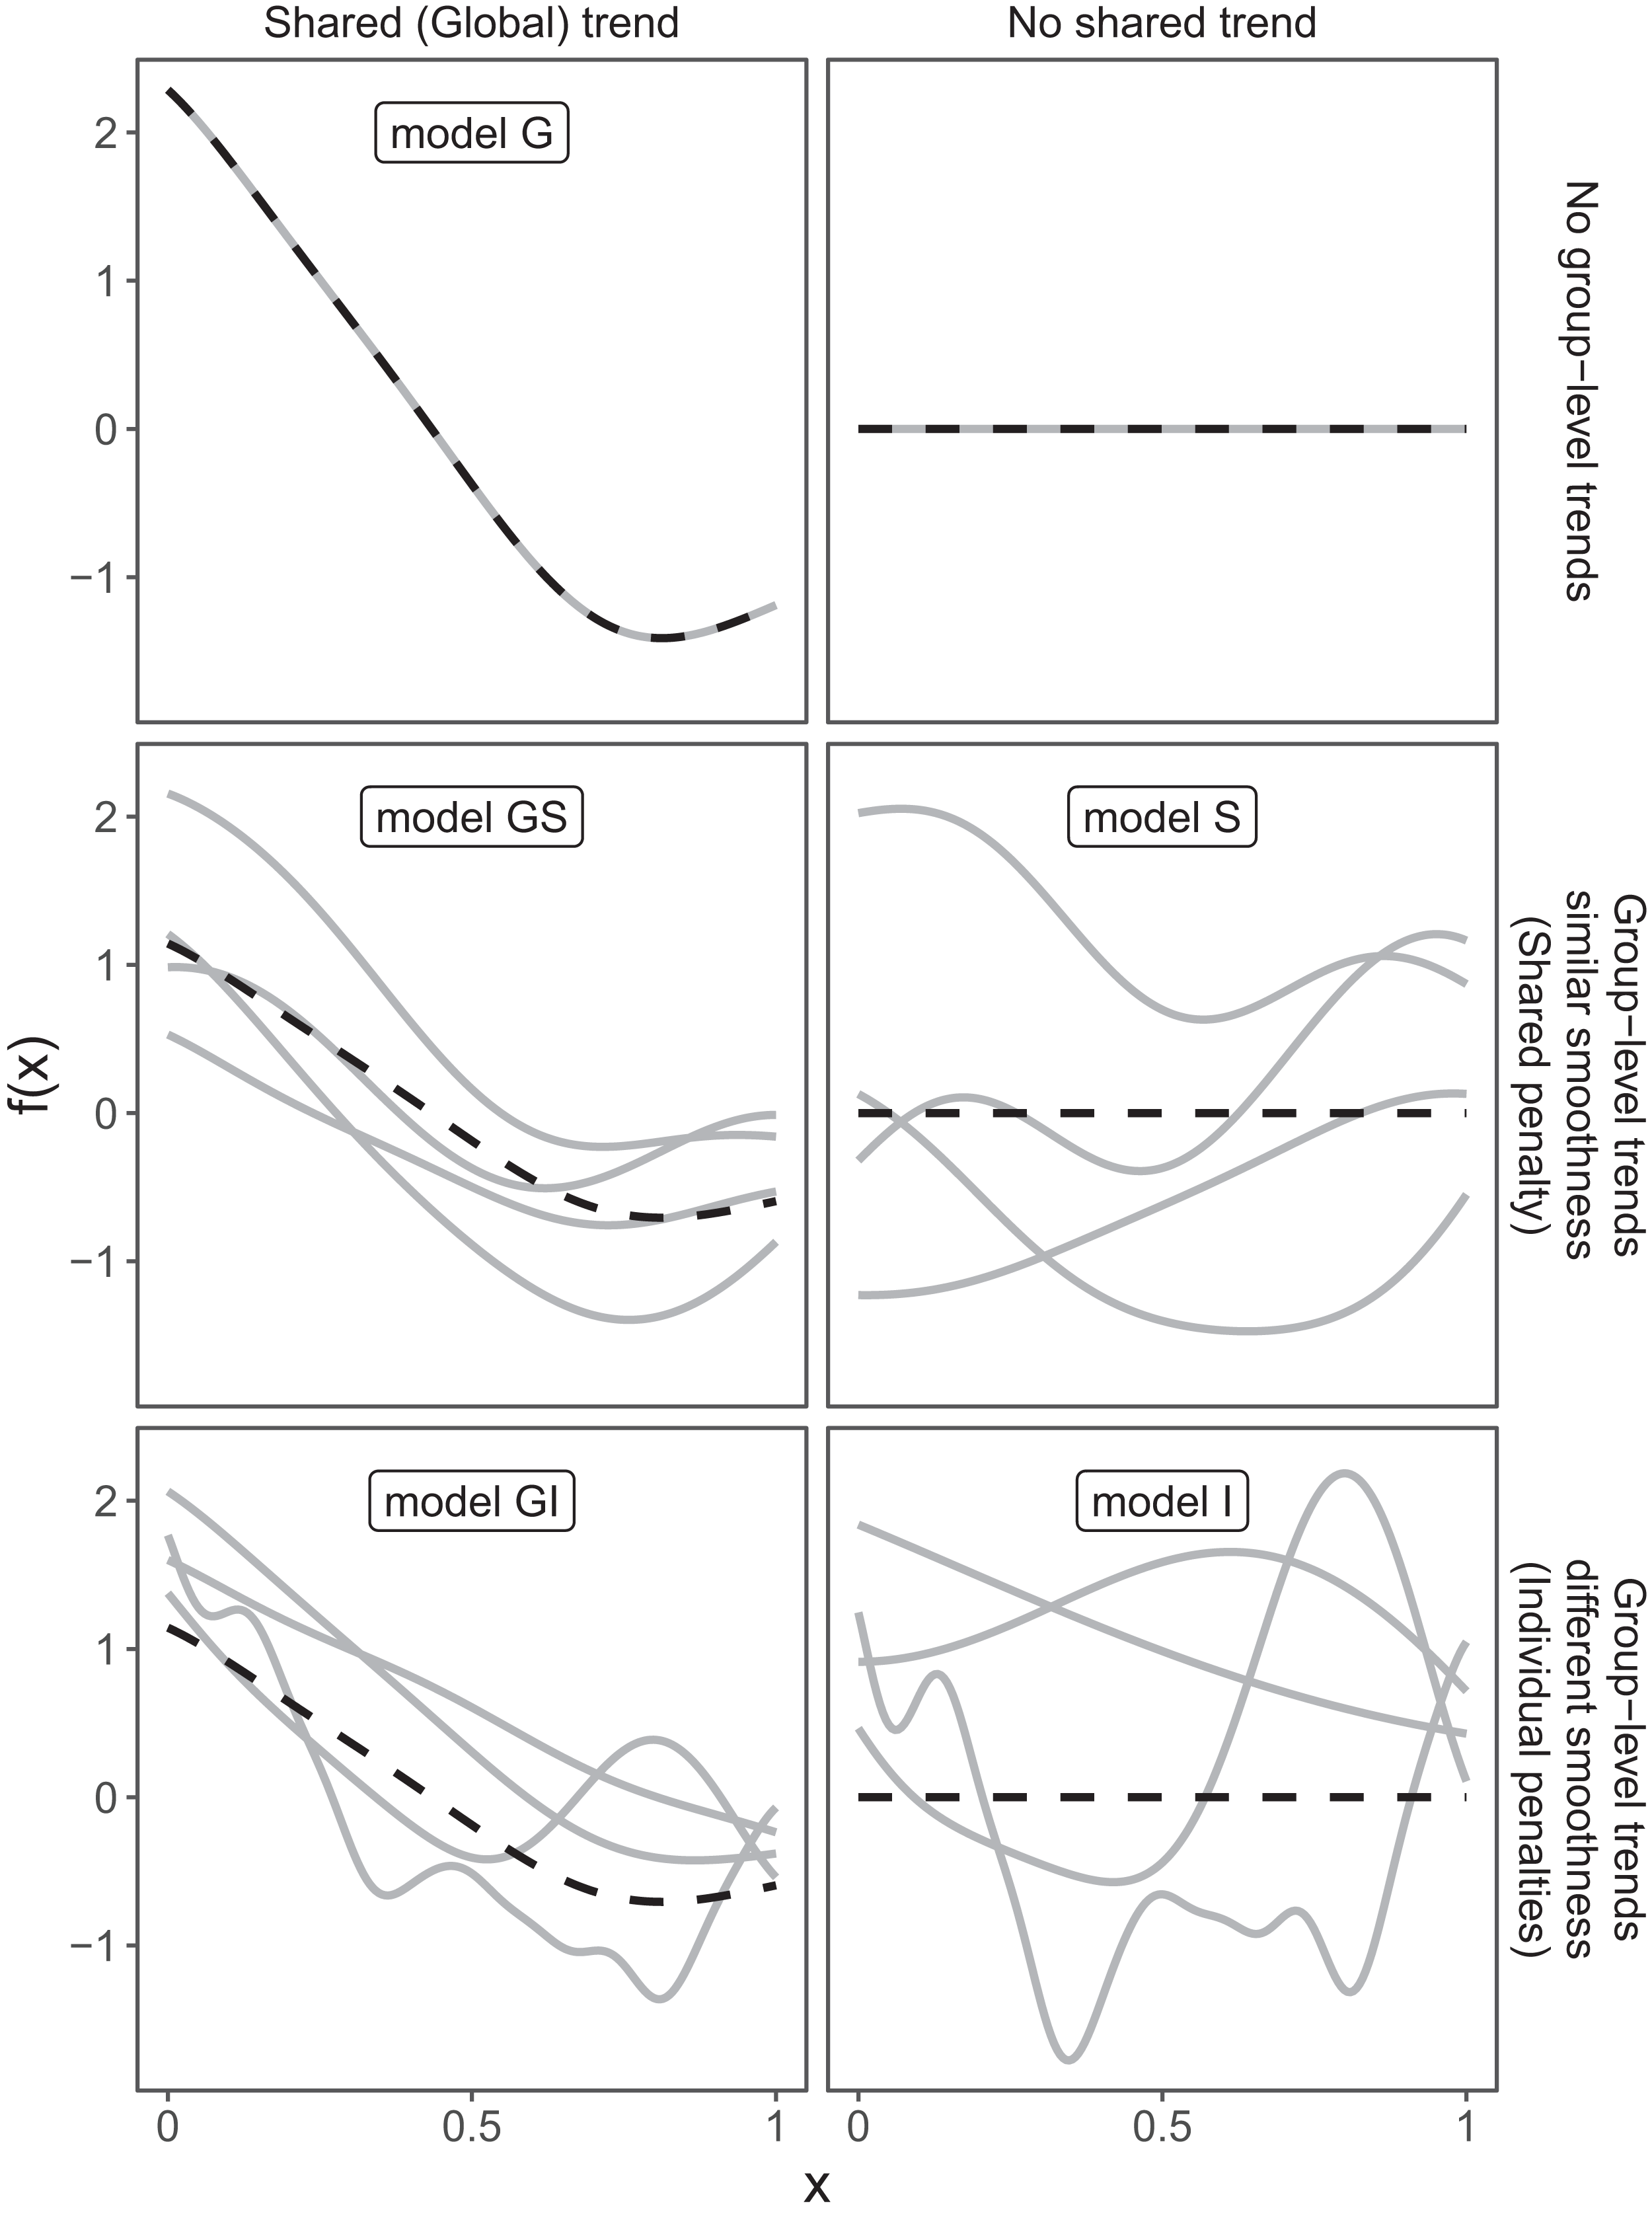
\includegraphics[width=34.72in]{../figures/HGAM} \caption{Alternate types of functional variation f(x) that can be fitted with HGAMs. Figure reproduced from: Pedersen EJ, Miller DL, Simpson GL, Ross N. 2019. Hierarchical generalized additive models in ecology: an introduction with mgcv. PeerJ 7:e6876 DOI: 10.7717/peerj.6876/fig-4}\label{fig:HGAM}
\end{figure}

\hypertarget{furthur-explaination-and-application-of-models}{%
\section{Furthur Explaination and Application of Models}\label{furthur-explaination-and-application-of-models}}

All models covered in this summary overview are explored in more detail
through an application to a single trail (Middle Cottonwood) in Section
\ref{MidCot}. Section \ref{AllTrailsAnalysis} contains an analysis of
all trails covered by trail-use cameras as well as a comparison of
several HGAM model structures.

\hypertarget{additional-resources}{%
\section{Additional Resources}\label{additional-resources}}

This summary pulls heavily from the following resources that are very
useful for a deeper dive into these models.

\begin{itemize}
\tightlist
\item
  \href{https://m-clark.github.io/generalized-additive-models/}{Generalized Additive
  Models}
\item
  \href{https://asbates.rbind.io/2019/02/04/what-are-splines/}{Simple overview of splines and basis
  functions}
\end{itemize}

\hypertarget{MidCot}{%
\chapter{Application to Middle Cottonwood Trail}\label{MidCot}}

In this section, we explore gradually more complicated model choices (each described in Section \ref{Models}) which we apply to a single trail (rather than then entire network of trails) so we can focus on understanding the model applied to these data.

We begin with a quick look at the data available for our chosen trail, Middle Cottonwood Trail. Then we will progress through several \texttt{ga(m)m} models that incorporate more complexity with each iteration. This will include a detailed overview of useful diagnostic tools, a look at what explanatory predictor variables should/could be included, as well as an example of how we may forecast (predict into the near future) using our chosen model.

\hypertarget{data-used}{%
\section{Data Used}\label{data-used}}

This 2.3-mile out-and-back trail was monitored via infrared counters between 2021-06-27 and 2021-08-16. This daily time series count data is combined with data from Strava Metro, and local weather data.

Strava Metro partners with Headwaters Economics to provide aggregated (daily, monthly, or annually) trail use information for the Bridgers. These data are broken into multiple edges within a single trail. Eight such edges are included for Middle Cottonwood. These edges do not represent independent observations as they represent trail use on connected locations and thus likely reflect the same trail users continuing along the trail. We summarize these data to a single value using the edge ID with the maximum observed number of trail numbers for a given day.

In another partnership, AllTrails has provided information on daily trail name searches for a subsection of trails (including Middle Cottonwood) in the Bridger Mountains.

Thus each row in the dataset details the following:

\begin{itemize}
\tightlist
\item
  the number of trail users for a given day
\item
  trail characteristics (trail name and number, location of trailhead)
\item
  counter characteristics (counter ID number, owner, location along trail)
\item
  Strava Metro information summarized to reflect the maximum count of all edges for a given day
\item
  AllTrails information on search term numbers for a given day
\item
  daily weather data (precipitation in inches, min/max temperature, AQI value, PM\(_{2.5}\) concentration)
\end{itemize}

Figure \ref{fig:MidCotTS} shows times series plot of counter and Strava trip counts, in addition to AllTrails search counts.

\begin{figure}

{\centering 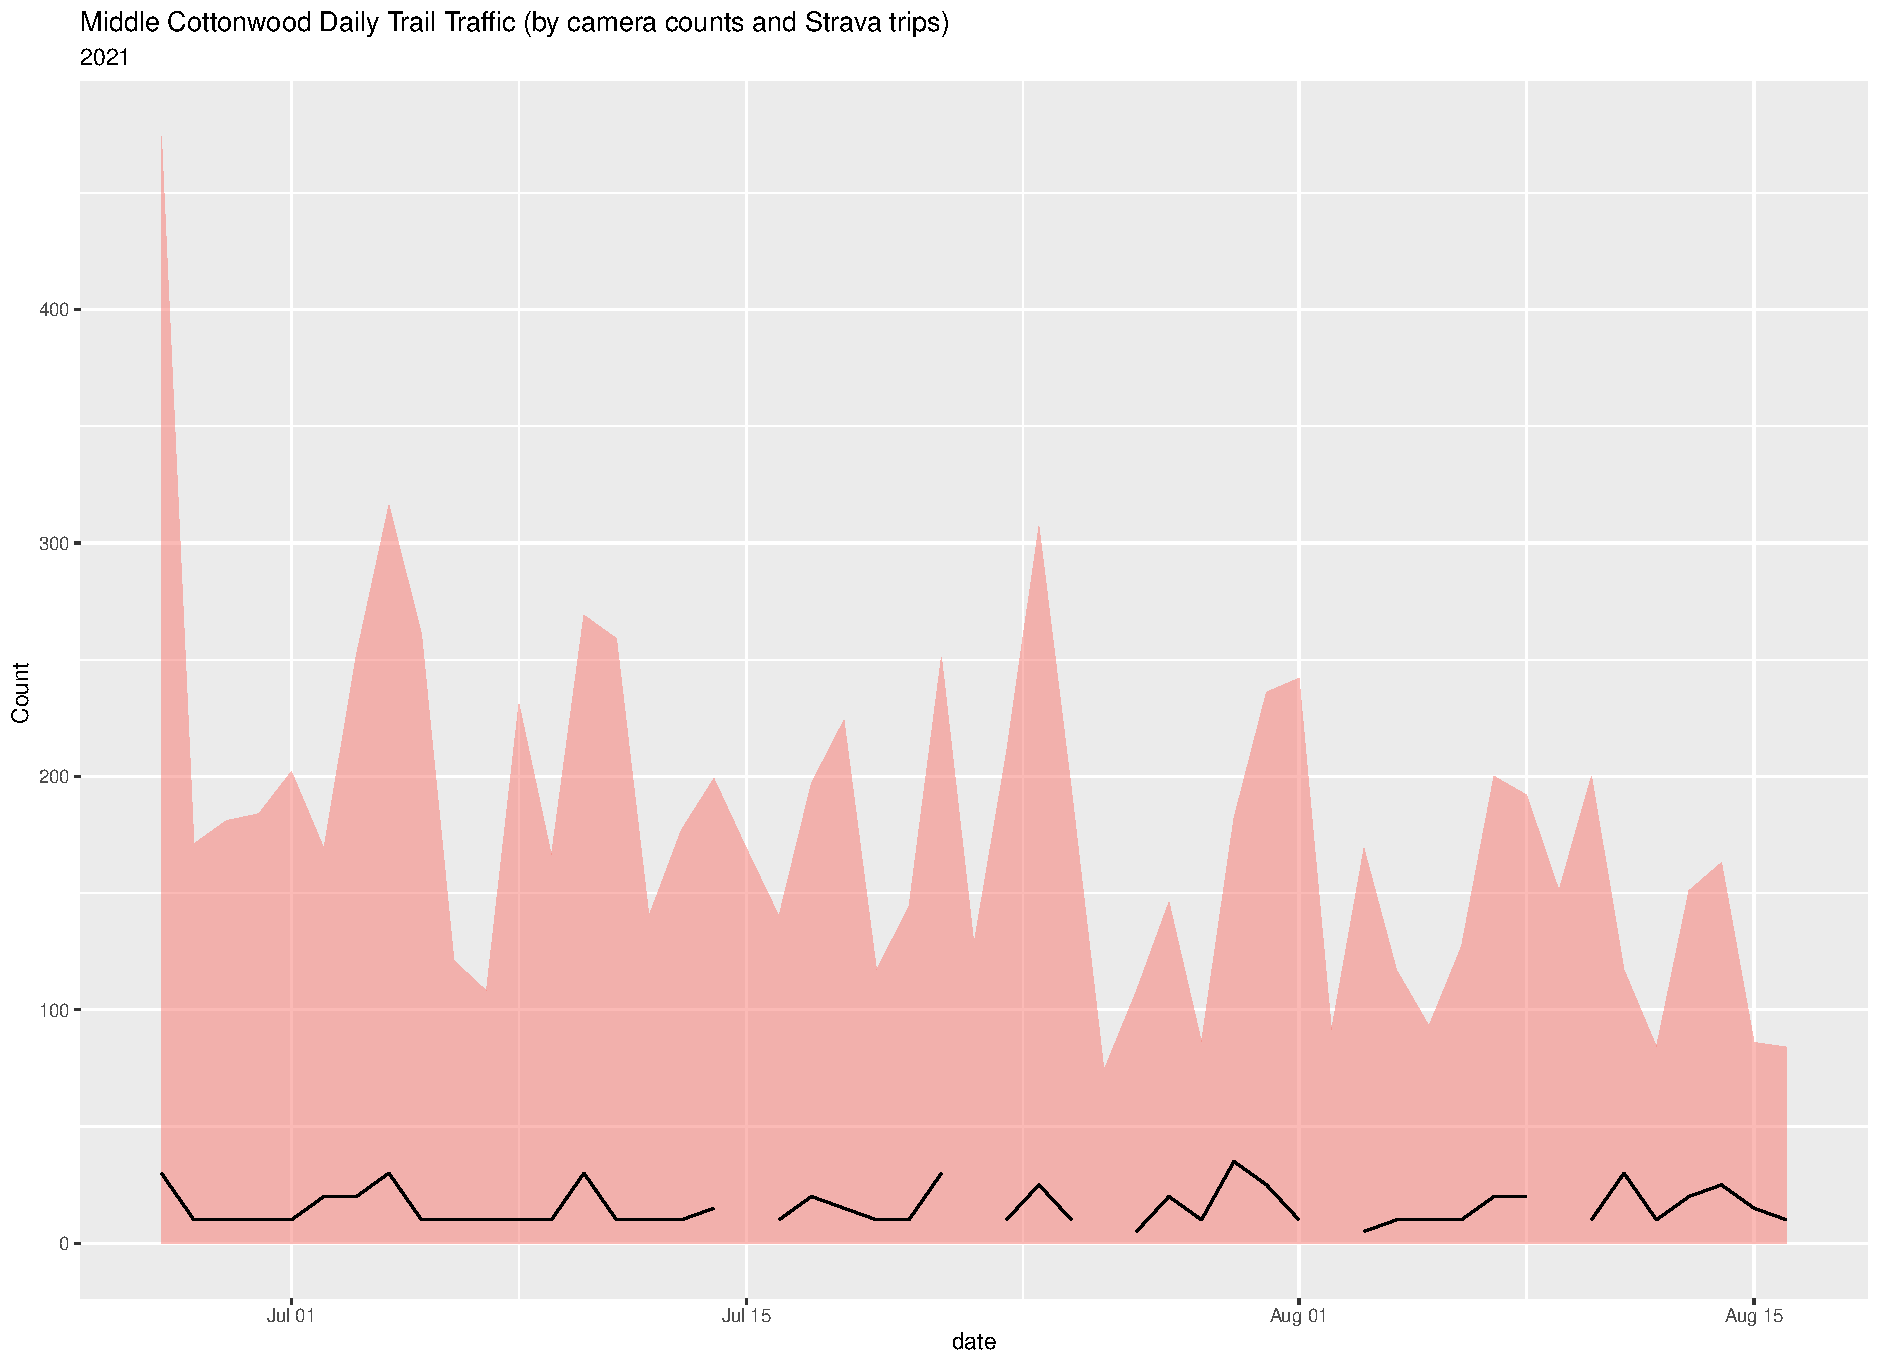
\includegraphics[width=1\linewidth]{../figures/MiddleCottonwood_TS} 

}

\caption{Daily trail traffic for Middle Cottonwood. Purple fill represents trail use counts from deployed counter cameras. Orange line represents trip counts per day provided by Strava Metro. Green line represents trail name searchs per day provided by AllTrails.}\label{fig:MidCotTS}
\end{figure}

We also examine the relationship between our response variable (max.camera, or the number of trips counted on a trail section per day) and several explanatory variables (Figure \ref{fig:covariates}).

\begin{figure}

{\centering 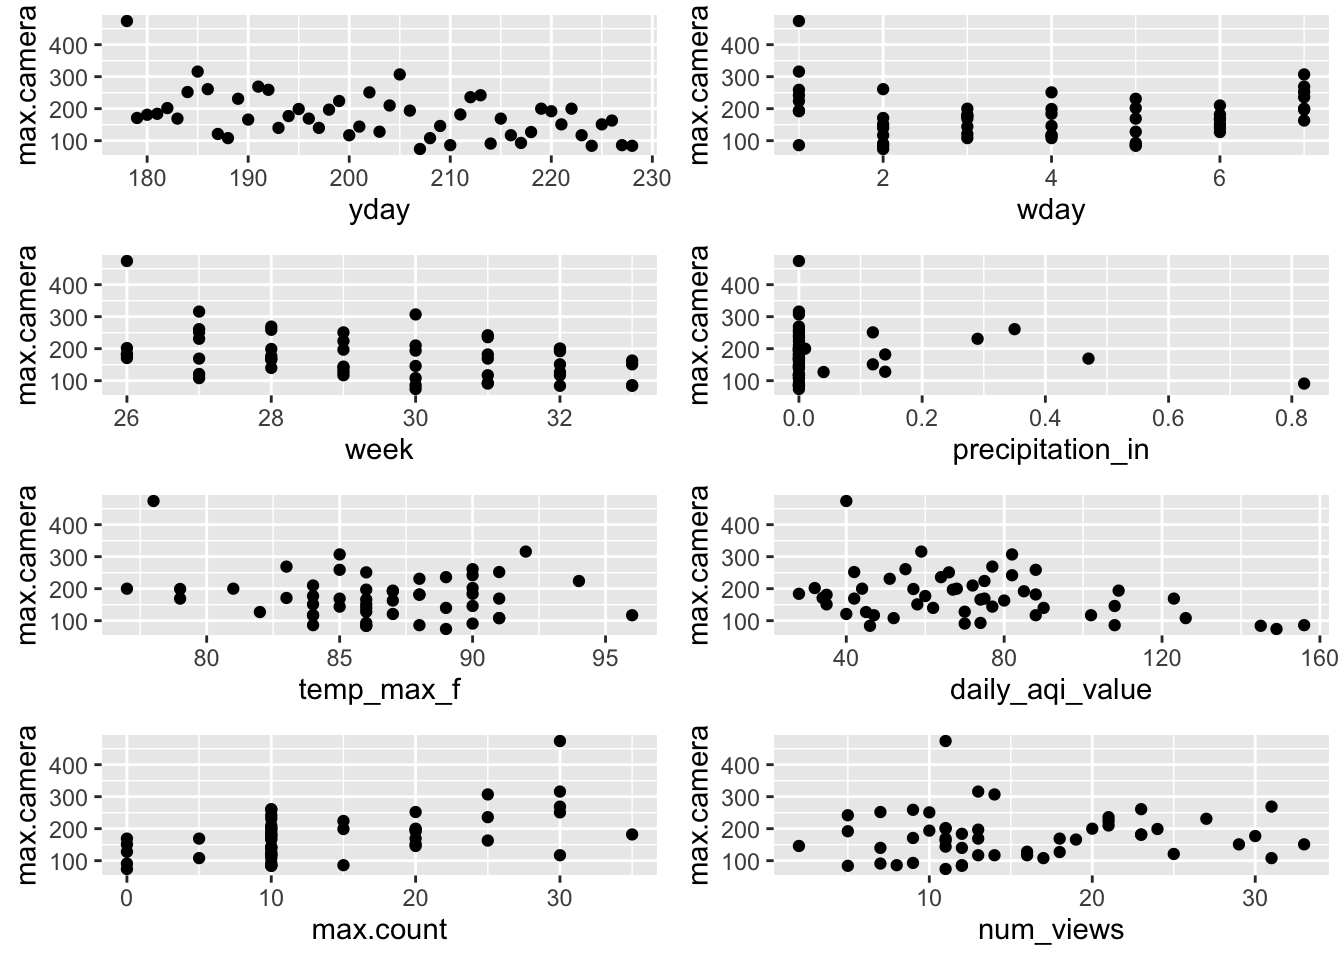
\includegraphics[width=1\linewidth]{Statistical-Analysis--Prediction-of-Trail-Use-in-Bridger-Mountains_files/figure-latex/covariates-1} 

}

\caption{Relationship of select covariates to trail use for Middle Cottonwood.}\label{fig:covariates}
\end{figure}

\hypertarget{model-options}{%
\section{Model Options}\label{model-options}}

The following provides a very brief overview of several different types of regression models. This material is by no means an exhaustive coverage of the topic (see Section \ref{Models}), but serves as an applied presentation allowing for us to build upon familiar modelling approaches towards what might be newer material.

All models are fit in R. GA(M)Ms are fit with the \textbf{mgcv} package \citep[\citet{R-Wood2}, \citet{R-Wood3}, \citet{R-Wood4}, \citet{R-Wood5}]{R-Wood1}.

\hypertarget{linear-regression-model-1}{%
\subsection{Linear Regression Model}\label{linear-regression-model-1}}

If we start simply and try to predict trail use count as our numeric response variable (\(y\)) via multiple linear regression (\texttt{lm}) using predictor variables, our model would have this general form:

\[
y = b_0 + b_1x_1 + b_2x_2 + \dots + \epsilon
\]

Translated in to \texttt{R} syntax, this model would look like:

\begin{Shaded}
\begin{Highlighting}[]
\NormalTok{lm\_mod }\OtherTok{\textless{}{-}} \FunctionTok{lm}\NormalTok{(max.camera }\SpecialCharTok{\textasciitilde{}} 
\NormalTok{               max.count }\SpecialCharTok{+} 
\NormalTok{               num\_views }\SpecialCharTok{+}
\NormalTok{               daily\_aqi\_value }\SpecialCharTok{+} 
\NormalTok{               precipitation\_in }\SpecialCharTok{+} 
\NormalTok{               temp\_max\_f, }
             \AttributeTok{data =}\NormalTok{ singleTrail)}

\FunctionTok{save}\NormalTok{(lm\_mod, }
     \AttributeTok{file=}\FunctionTok{here}\NormalTok{(}\StringTok{"output/models/singleT\_lm.rda"}\NormalTok{), }
     \AttributeTok{compress=}\StringTok{\textquotesingle{}xz\textquotesingle{}}\NormalTok{)}
\end{Highlighting}
\end{Shaded}

This model assumes linear relationships between variables, a Gaussian (normal) distribution for the response variable, AND independent observations - \textbf{all of which are unlikely to be met with our data.}

\hypertarget{generalized-linear-regression-model-1}{%
\subsection{Generalized Linear Regression Model}\label{generalized-linear-regression-model-1}}

To address the issue of violated normality assumption in the previous model we can try a generalized linear model (\texttt{glm}) with a Poisson distribution (log link). The trail use count response is strictly non-negative and discrete (e.g.~can't have 13.5 trail users). This model, using R syntax, would have this form:

\begin{Shaded}
\begin{Highlighting}[]
\NormalTok{glm\_mod }\OtherTok{\textless{}{-}} \FunctionTok{glm}\NormalTok{(max.camera }\SpecialCharTok{\textasciitilde{}} 
\NormalTok{                 max.count }\SpecialCharTok{+} 
\NormalTok{                 num\_views }\SpecialCharTok{+}
\NormalTok{                 daily\_aqi\_value }\SpecialCharTok{+} 
\NormalTok{                 precipitation\_in }\SpecialCharTok{+} 
\NormalTok{                 temp\_max\_f, }
               \AttributeTok{data =}\NormalTok{ singleTrail, }
               \AttributeTok{family =}\NormalTok{ poisson)}

\FunctionTok{save}\NormalTok{(glm\_mod, }
     \AttributeTok{file=}\FunctionTok{here}\NormalTok{(}\StringTok{"output/models/singleT\_glm.rda"}\NormalTok{), }
     \AttributeTok{compress=}\StringTok{\textquotesingle{}xz\textquotesingle{}}\NormalTok{)}
\end{Highlighting}
\end{Shaded}

However, this does not address the non-linear relationship between response and predictors, nor the (temporal) dependence between observations.

\hypertarget{generalized-additive-models}{%
\subsection{Generalized Additive Models}\label{generalized-additive-models}}

We can address non-linearity through a simple generalized additive model (\texttt{gam}) with the general form,

\[
y = b_0 + f_1(x_1) + f_2(x_2)\dots + \epsilon
\]
and the R syntax form of:

\begin{Shaded}
\begin{Highlighting}[]
\NormalTok{gam\_mod }\OtherTok{\textless{}{-}}\NormalTok{ mgcv}\SpecialCharTok{::}\FunctionTok{gam}\NormalTok{(max.camera }\SpecialCharTok{\textasciitilde{}} 
\NormalTok{                       max.count }\SpecialCharTok{+}
\NormalTok{                       num\_views }\SpecialCharTok{+}
                       \FunctionTok{s}\NormalTok{(yday, }\AttributeTok{bs =} \StringTok{"cc"}\NormalTok{) }\SpecialCharTok{+} 
                       \FunctionTok{s}\NormalTok{(wday, }\AttributeTok{bs =} \StringTok{"cc"}\NormalTok{,  }\AttributeTok{k =} \DecValTok{7}\NormalTok{) }\SpecialCharTok{+}
                       \FunctionTok{s}\NormalTok{(month, }\AttributeTok{k =} \DecValTok{3}\NormalTok{), }
                     \AttributeTok{data =}\NormalTok{ singleTrail, }
                     \AttributeTok{knots =} \FunctionTok{list}\NormalTok{(}\AttributeTok{yday =} \FunctionTok{c}\NormalTok{(}\DecValTok{0}\NormalTok{,}\DecValTok{365}\NormalTok{)),}
                     \AttributeTok{method =} \StringTok{\textquotesingle{}REML\textquotesingle{}}\NormalTok{,}
                     \AttributeTok{family =}\NormalTok{ poisson)}

\FunctionTok{save}\NormalTok{(gam\_mod, }
     \AttributeTok{file=}\FunctionTok{here}\NormalTok{(}\StringTok{"output/models/singleT\_gam.rda"}\NormalTok{), }
     \AttributeTok{compress=}\StringTok{\textquotesingle{}xz\textquotesingle{}}\NormalTok{)}
\end{Highlighting}
\end{Shaded}

In the above code we fit a \texttt{gam} which is non-linear in \texttt{yday}, \texttt{wday}, and \texttt{month} but we also include \texttt{max.count} (Strava number of trips) and \texttt{num\_views} (AllTrails searches) as linear terms. Note that these variable does not have the \texttt{s} prefix indicating a (spline based) smoothing term.

We specified basis functions for the day of year (\texttt{yday}) and day of week variable (\texttt{wday}). The code \texttt{bs="cc"} indicates that we are selecting a cyclic cubic regression spline, which is a penalized cubic regression spine whose ends match up. In the context of day of week we know that Sunday/Saturday would be the `ends' that `match' together. If we do not specify any, the default basis function is thin plate splines. They are the default smooth for \texttt{s} terms because there is a defined sense in which they are the optimal smoother of any given basis dimension/rank (\citep{R-Wood5}). One key advantage of this approach is that it avoids the knot placement problems of conventional regression spline modelling.

We have also specified the number of knots, \(k\), for both wday and month. If we do not specify \(k\) then the default is 10. In both of these cases this results in the following errors:

\begin{quote}
Error in place.knots(x, nk) :
more knots than unique data values is not allowed

Error in smooth.construct.tp.smooth.spec(object, dk\$data, dk\$knots) :
A term has fewer unique covariate combinations than specified maximum degrees of freedom
\end{quote}

(I believe the error messages are different due to differing basis functions.) For the \texttt{wday} variable we know that there's only 7 unique values (for each day of the week) and thus this is the highest value of \(k\) able to be used. Similarly, these data cover 3 \texttt{month} values and so that is our selection for \(k\) in this instance.

\hypertarget{generalized-additive-mixed-models}{%
\subsection{Generalized Additive Mixed Models}\label{generalized-additive-mixed-models}}

Recall that an assumption of the \texttt{gam} model is that observations are \textbf{conditionally} independent. Unless we specify that the data aren't independent using \texttt{gamm} instead of \texttt{gam}, the \texttt{gam} model will perform smoothness selection assuming that we have \(n\) independent observations.
We first fit a \texttt{gamm} model to the exact same covariates and we used when fitting the previous \texttt{gam} model. The \texttt{R} syntax is as follows:

However, we may also include some more explanatory variables to better reflect our understanding of this system we are modelling. The following \texttt{gamm} model has additional non-linear terms included pulling from local weather information. We have specified \texttt{k=9} for \texttt{precipiation\_in} again because the default value of 10 is too high and results in an error message and the code fails to run.

\hypertarget{gamm-with-additional-temporal-autocorrelation-specification}{%
\subsection{GAMM with additional temporal autocorrelation specification}\label{gamm-with-additional-temporal-autocorrelation-specification}}

If we model temporal autocorrelation through temporal terms in the model (as we did in \texttt{gamm\_mod2}), then the smooth functions of temporal variables (such as \texttt{yday}, \texttt{wday}, etc) could be already accounting for the temporal structure in the data such that once we consider the model, the observations are independent. Note that it's also possible that the temporal autocorrelation is \textbf{not} captured through the terms in the model and additional complexity would be beneficial.

Autocorrelation is meant to capture either temporal or spatial dependence in a model. With a \texttt{ga(m)m} approach we consider both autocorrelation and a moving average (MA) process. An autoregressive process (AR(\(n\))) is one in which the previous \(n\) points influence the current observations. A moving average (MA) process is one in which the current value is an average of preceding white noise. We are most interested in the main (fixed) effects of our model, while any autocorrelation is ancillary, but necessary to include.

For optimal choose of AR(p) and MA(q) orders \texttt{auto.arima} function, from the \textbf{forecast} package \citep[\citet{R-forecast2}]{R-forecast}, is used on (normalized) residuals from the model fits. It automatically chooses optimal orders of ARMA (in our case) based on AIC criterion. As we can use just ARMA models in gamm, so nonstationarity isn't allowed, we set an argument stationary = TRUE.

\begin{Shaded}
\begin{Highlighting}[]
\DocumentationTok{\#\#find values for p and q in the ARMA model }
\NormalTok{arma\_res }\OtherTok{\textless{}{-}}\NormalTok{ forecast}\SpecialCharTok{::}\FunctionTok{auto.arima}\NormalTok{(}\FunctionTok{resid}\NormalTok{(gamm\_mod2}\SpecialCharTok{$}\NormalTok{lme, }
                                          \AttributeTok{type =} \StringTok{"normalized"}\NormalTok{),}
                                 \AttributeTok{stationary =} \ConstantTok{TRUE}\NormalTok{,}
                                 \AttributeTok{seasonal =} \ConstantTok{TRUE}\NormalTok{)}

 \CommentTok{\#here there\textquotesingle{}s no output bc an AR1 structure is sufficient, but in other instances }
\CommentTok{\# this shows what values for p and q to choose}
\NormalTok{arma\_res}\SpecialCharTok{$}\NormalTok{coef}
\end{Highlighting}
\end{Shaded}

\begin{Shaded}
\begin{Highlighting}[]
 \DocumentationTok{\#\# AR(1)}
\NormalTok{gamm\_mod2\_AR1 }\OtherTok{\textless{}{-}} \FunctionTok{gamm}\NormalTok{(max.camera }\SpecialCharTok{\textasciitilde{}} 
                        \FunctionTok{s}\NormalTok{(yday) }\SpecialCharTok{+}
                        \FunctionTok{s}\NormalTok{(month, }\AttributeTok{k =} \DecValTok{3}\NormalTok{) }\SpecialCharTok{+}
                        \FunctionTok{s}\NormalTok{(wday, }
                          \AttributeTok{bs =} \StringTok{"cc"}\NormalTok{, }\AttributeTok{k =} \DecValTok{7}\NormalTok{) }\SpecialCharTok{+}
                        \FunctionTok{s}\NormalTok{(daily\_aqi\_value) }\SpecialCharTok{+}
                        \FunctionTok{s}\NormalTok{(temp\_max\_f, }\AttributeTok{k =} \DecValTok{5}\NormalTok{) }\SpecialCharTok{+}
                        \FunctionTok{s}\NormalTok{(precipitation\_in, }\AttributeTok{k =} \DecValTok{5}\NormalTok{) }\SpecialCharTok{+}
\NormalTok{                        max.count }\SpecialCharTok{+} 
\NormalTok{                        num\_views,}
              \AttributeTok{data =}\NormalTok{ singleTrail, }
              \AttributeTok{family =}\NormalTok{ poisson,}
              \AttributeTok{correlation =} \FunctionTok{corAR1}\NormalTok{(}\AttributeTok{form =} \SpecialCharTok{\textasciitilde{}}\NormalTok{ yday),}
              \AttributeTok{method =} \StringTok{"REML"}\NormalTok{)}
\end{Highlighting}
\end{Shaded}

\begin{verbatim}
## 
##  Maximum number of PQL iterations:  20
\end{verbatim}

\begin{Shaded}
\begin{Highlighting}[]
\FunctionTok{save}\NormalTok{(gamm\_mod2\_AR1, }
     \AttributeTok{file=}\FunctionTok{here}\NormalTok{(}\StringTok{"output/models/singleT\_gamm{-}Ar1.rda"}\NormalTok{), }
     \AttributeTok{compress=}\StringTok{\textquotesingle{}xz\textquotesingle{}}\NormalTok{)}
\end{Highlighting}
\end{Shaded}

Even with the use of \texttt{auto.arima} we must still examine diagnostic plots (in this case, ACF and PACF plots for identifying autocorrelation) and summaries for each model (see Section \ref{Diag} for more details).

\hypertarget{why-not-a-classic-time-series-analysis}{%
\subsection{Why not a Classic Time Series Analysis?}\label{why-not-a-classic-time-series-analysis}}

While both times series regression and GAM's can both be applied to temporal data, the two models are fundamentally different. Time series regression makes an assumption of a stationary series, while GAM deals with the trend internally with smoothing. With GAM, the estimated smoother is detrending the data and the (stationary) residuals are subjected to an ARMA model. The use of GAMs is useful when one is interested in estimating the trends in time series data and those trends are, in general, non-linear. In classical time series modelling, the interest is in modelling data as stochastic trends using lagged versions of the response and/or current and lagged versions of a white noise process.

\hypertarget{Diag}{%
\section{Diagnostic Practices}\label{Diag}}

Once a model (or a suite of models) is fit, we need to take a more detailed look at model outputs to learn how to interpret the results of our model-fitting and better understand the relationships between variables.

\hypertarget{summarize}{%
\subsection{Summarize}\label{summarize}}

We start with the \texttt{summary()} function which may be applied to a \texttt{gam} object in R. Below we have the summary output for our \texttt{gamm} model with explanatory variables.

\begin{Shaded}
\begin{Highlighting}[]
\CommentTok{\# summary(lm\_mod)}
\CommentTok{\# summary(glm\_mod)}
\CommentTok{\# summary(gam\_mod)}
\CommentTok{\# summary(gam\_mod2)}
\CommentTok{\# summary(gamm\_mod$gam)}
\FunctionTok{summary}\NormalTok{(gamm\_mod2}\SpecialCharTok{$}\NormalTok{gam)}
\end{Highlighting}
\end{Shaded}

\begin{verbatim}
## 
## Family: poisson 
## Link function: log 
## 
## Formula:
## max.camera ~ s(yday, bs = "cc") + s(month, k = 3) + s(wday, bs = "cc", 
##     k = 7) + s(daily_aqi_value) + s(temp_max_f) + s(precipitation_in, 
##     k = 9) + max.count + num_views
## 
## Parametric coefficients:
##             Estimate Std. Error t value Pr(>|t|)    
## (Intercept) 4.943373   0.057037  86.670  < 2e-16 ***
## max.count   0.007160   0.002287   3.130  0.00581 ** 
## num_views   0.004407   0.003010   1.464  0.16051    
## ---
## Signif. codes:  0 '***' 0.001 '**' 0.01 '*' 0.05 '.' 0.1 ' ' 1
## 
## Approximate significance of smooth terms:
##                       edf Ref.df      F  p-value    
## s(yday)             5.955  8.000  5.103 0.000490 ***
## s(month)            1.000  1.000  8.798 0.008270 ** 
## s(wday)             4.621  5.000 30.473  < 2e-16 ***
## s(daily_aqi_value)  5.838  5.838  9.269 0.000119 ***
## s(temp_max_f)       6.485  6.485 13.780 1.14e-05 ***
## s(precipitation_in) 6.189  6.189 13.053 6.85e-06 ***
## ---
## Signif. codes:  0 '***' 0.001 '**' 0.01 '*' 0.05 '.' 0.1 ' ' 1
## 
## R-sq.(adj) =  0.897   
##   Scale est. = 1         n = 51
\end{verbatim}

\begin{Shaded}
\begin{Highlighting}[]
\CommentTok{\# summary(gamm\_mod2\_AR1$gam)}
\CommentTok{\# summary(gamm\_mod2\_ARMA$gam)}
\end{Highlighting}
\end{Shaded}

The first part of the summary describes the model we fit. The ``Family'' component tells us the model assumes a Poisson distribution of our response, and the ``Link'' of ``log'' shows that the model transforms the predictions.

The next section describes the parametric terms of our model, referring to the linear terms in the model. This section may be familiar from linear modeling. It shows the coefficients for the linear terms in the model, their values, errors, test statistics, and p-values. Asterisks next to the p-values indicate statistical significance. In this case, the model intercept is significant, and the fixed effect of max.count (the number of aggregated/binned Strava trip counts) is also significant at the 0 level. However, the fixed effect of num\_views (trail name searches in AllTrails) is not significant for Middle Cottonwood.

The next section covers smooth terms. For these smooths the summary for coefficients is not printed. This is because each smooth has coefficients for each basis function. Instead, the first column reads edf, which stands for effective degrees of freedom. This value represents the complexity of the smooth. An edf of 1 is equivalent to a straight line. An edf of 2 is equivalent to a quadratic curve, and so on, with higher edfs describing more wiggly curves. In our summary, all included smooth terms are significant at the 0.001 level. Note that the `month' term has an edf of 1, indicating the smooth is equivalent to a straight line. The day of year term (`yday') has the highest edf (8.338) and thus highest wiggliness. These edf values (and wiggliness) for each smoothing term may be compared to the corresponding partial effects plot in Figure \ref{fig:MCdraw}.

The terms to the right of the EDF column have to do with significance testing for smooths. The Ref.df and F columns are test statistics used in an ANOVA test to test overall significance of the smooth. The result of this test is the p-value to the right. It's important to note that these values are approximate, and it's important to visualize your model to check them.

The R-sq(adj.) does not a straight-forward interpretation of a measure of ``proportion of variance explained'' in nonlinear regression, and thus can not be employed as an absolute measure of model performance. Deviance explained should be a more generalized measurement of goodness of fit especially for non-gaussian models (such as we have here).

The scale estimate is \(\hat{\phi}\) , i.e.~this is the value of \(\phi\) estimated during model fitting. For the Poisson and Binomial families/distributions, by definition \(\phi\)=1, but for other distributions this is not the case, including the Gaussian. In the Gaussian case, \(\hat{\phi}\) is the residual standard error squared.

\hypertarget{visualize}{%
\subsection{Visualize}\label{visualize}}

After examining the summary, we should visualize our results. This may be accomplished using the several available function, however we choose to use the \textbf{gratia} package \citep{R-gratia} to produce these plots in \textbf{ggplot2} rather than base R.

\hypertarget{draw}{%
\subsubsection{Draw}\label{draw}}

\begin{Shaded}
\begin{Highlighting}[]
\CommentTok{\# gratia::draw(gam\_mod, residuals = T)}
\CommentTok{\# gratia::draw(gam\_mod2, residuals = T)}
\CommentTok{\# gratia::draw(gamm\_mod, residuals = T)}
\NormalTok{gratia}\SpecialCharTok{::}\FunctionTok{draw}\NormalTok{(gamm\_mod2, }\AttributeTok{residuals =}\NormalTok{ T)}
\end{Highlighting}
\end{Shaded}

\begin{figure}

{\centering 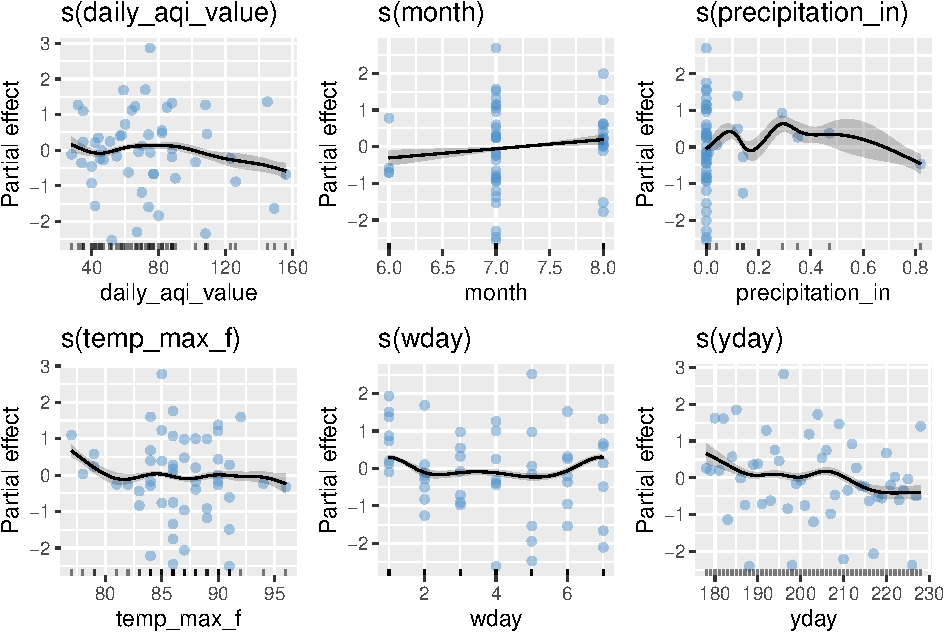
\includegraphics{Statistical-Analysis--Prediction-of-Trail-Use-in-Bridger-Mountains_files/figure-latex/MCdraw-1} 

}

\caption{Plots of estimated smooths from the model fit with Middle Cottonwood trail use count data only.}\label{fig:MCdraw}
\end{figure}

The plots (Figure \ref{fig:MCdraw} generated by \textbf{gratia}'s draw() (or \textbf{mgcv}'s plot() in base R graphics) function are partial effect plots. These may help diagnose problems with the model, such as oversmoothing. These plots show the component effect of each of the smooth or linear terms in the model, which add up to the overall prediction (summed effect). We often want to show data alongside model predictions. These plots aid in this by (1) including covariate values along the bottom axis of the plots and (2) plotting partial residuals (here in light blue) on the plots. Partial residuals are the difference between the partial effect and the data, after all other partial effects have been accounted for. These plots also include shading representing 95\% confidence interval for the mean shape of the effect.

\hypertarget{gam-check}{%
\subsubsection{GAM Check}\label{gam-check}}

Running gam.check() on a model provides several outputs, in both the console and as plots. We'll start with the console output. First, gam.check() reports on model convergence. Here, it immediately provides a warning against interpreting these results when applied to a \texttt{gamm} based fit. We include this check here mainly to note this restriction and the usefulness if a \texttt{gam} fit is appropriate.

Below, we see a table of basis checking results. This shows a statistical test for patterns in model residuals, which should be random. Each line reports the test results for one smooth. It shows the k value or number of basis functions, the effective degrees of freedom, a test statistic, and p-value.

Here, small p-values indicate that residuals are not randomly distributed. This often means there are not enough basis functions.

This is an approximate test. Always visualize your results too, and compare the k and edf values in addition to looking at the p-value.

\begin{Shaded}
\begin{Highlighting}[]
\CommentTok{\# gam.check(gam\_mod)}
\CommentTok{\# gam.check(gam\_mod2)}
\FunctionTok{layout}\NormalTok{(}\FunctionTok{matrix}\NormalTok{(}\DecValTok{1}\SpecialCharTok{:}\DecValTok{4}\NormalTok{, }\AttributeTok{ncol =} \DecValTok{2}\NormalTok{))}
\FunctionTok{gam.check}\NormalTok{(gamm\_mod2}\SpecialCharTok{$}\NormalTok{gam)}
\end{Highlighting}
\end{Shaded}

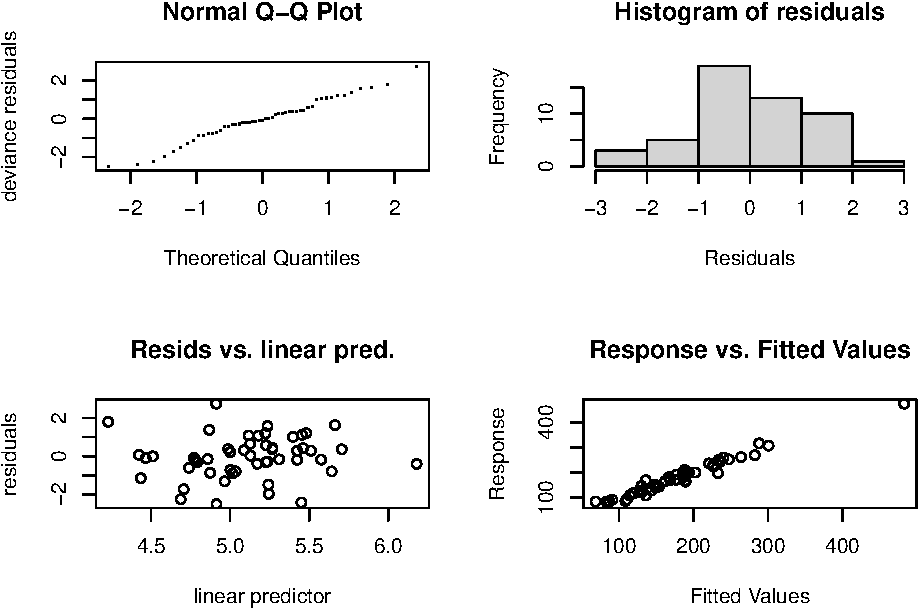
\includegraphics{Statistical-Analysis--Prediction-of-Trail-Use-in-Bridger-Mountains_files/figure-latex/unnamed-chunk-8-1.pdf}

\begin{verbatim}
## 
## 'gamm' based fit - care required with interpretation.
## Checks based on working residuals may be misleading.
## Basis dimension (k) checking results. Low p-value (k-index<1) may
## indicate that k is too low, especially if edf is close to k'.
## 
##                       k'  edf k-index p-value
## s(yday)             8.00 5.96    1.14    0.80
## s(month)            2.00 1.00    1.14    0.81
## s(wday)             5.00 4.62    0.87    0.17
## s(daily_aqi_value)  9.00 5.84    1.18    0.88
## s(temp_max_f)       9.00 6.49    1.16    0.85
## s(precipitation_in) 8.00 6.19    1.22    0.91
\end{verbatim}

\begin{Shaded}
\begin{Highlighting}[]
\FunctionTok{layout}\NormalTok{(}\DecValTok{1}\NormalTok{)}
\end{Highlighting}
\end{Shaded}

Each of these plot outputs gives a different way of looking at your model residuals. These plots show the results from the original, poorly fit model. On the top-left is a Q-Q plot, which compares the model residuals to a normal distribution. A well-fit model's residuals will be close to a straight line. On bottom left is a histogram of residuals. We would expect this to have a symmetrical bell shape. On top-right is a plot of residual values. These should be evenly distributed around zero. Finally, on the bottom-right is plot of response against fitted values. A perfect model would form a straight line. We don't expect a perfect model, but we do expect the pattern to cluster around the 1-to-1 line.

\hypertarget{appraise}{%
\subsubsection{Appraise}\label{appraise}}

The \texttt{appraise}() function provides another way to obtain standard diagnotic plots for GAMs.

The plots produced are (from left-to-right, top-to-bottom),

\begin{itemize}
\tightlist
\item
  quantile-quantile (QQ) plot of deviance residuals,
\item
  scatterplot of deviance residuals against the linear predictor,
\item
  histogram of deviance residuals, and
\item
  scatterplot of observed vs fitted values.
\end{itemize}

\begin{Shaded}
\begin{Highlighting}[]
\CommentTok{\# gratia::appraise(gam\_mod)}
\CommentTok{\# gratia::appraise(gam\_mod2)}
\CommentTok{\# gratia::appraise(gamm\_mod$gam)}
\NormalTok{gratia}\SpecialCharTok{::}\FunctionTok{appraise}\NormalTok{(gamm\_mod2}\SpecialCharTok{$}\NormalTok{gam)}
\end{Highlighting}
\end{Shaded}

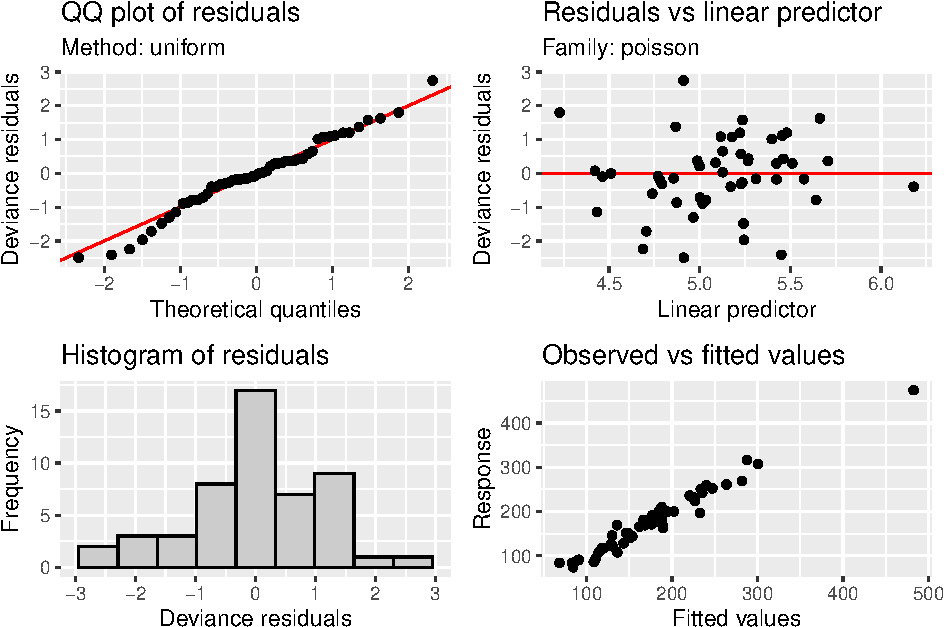
\includegraphics{Statistical-Analysis--Prediction-of-Trail-Use-in-Bridger-Mountains_files/figure-latex/unnamed-chunk-9-1.pdf}

Fitted vs.~response plots are generally less useful for non-normally distributed data as it can be difficult to visually assess if the observed data shows more heteroskedasticity than expected.

\hypertarget{time-series-gamm-diagnostic-plots}{%
\subsubsection{Time Series GAMM Diagnostic Plots}\label{time-series-gamm-diagnostic-plots}}

The following plots are a combination of various residuals plots and ACF plots produced with a bespoke R function created by Gavin Simpson and hosted on GitHub at: \url{https://github.com/gavinsimpson/random_code/blob/master/tsDiagGamm.R}. This function creates diagnostic plots specifically for time series data fit with a \texttt{gamm}, as we have with our trail use data.

\begin{Shaded}
\begin{Highlighting}[]
\NormalTok{singleTrail\_dropna }\OtherTok{\textless{}{-}}\NormalTok{ singleTrail }\SpecialCharTok{\%\textgreater{}\%} 
\NormalTok{  tidyr}\SpecialCharTok{::}\FunctionTok{drop\_na}\NormalTok{(}\StringTok{\textquotesingle{}daily\_aqi\_value\textquotesingle{}}\NormalTok{)}

\FunctionTok{with}\NormalTok{(singleTrail\_dropna, }
     \FunctionTok{tsDiagGamm}\NormalTok{(gamm\_mod2, }
                \AttributeTok{timevar =}\NormalTok{ yday,}
                \AttributeTok{observed =}\NormalTok{ max.camera))}
\end{Highlighting}
\end{Shaded}

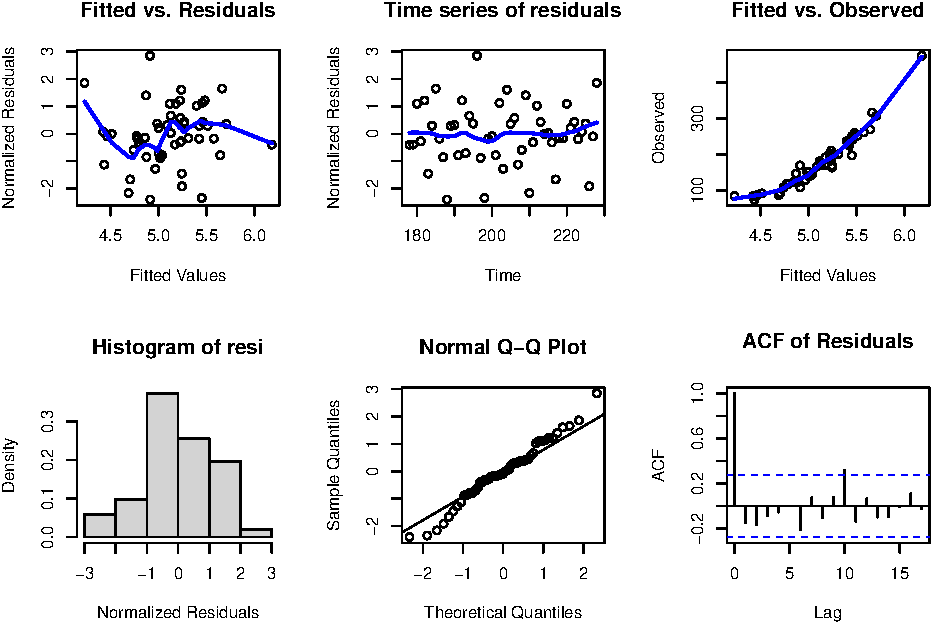
\includegraphics{Statistical-Analysis--Prediction-of-Trail-Use-in-Bridger-Mountains_files/figure-latex/tsDiagGAMM-1.pdf}

\hypertarget{rootogram}{%
\subsubsection{Rootogram}\label{rootogram}}

A good way to check how well the model compares with the observed data (and hence check for over-dispersion in the data relative to the conditional distribution implied by the model) is via a rootogram. A rootogram is a model diagnostic tool that assesses the goodness of fit of a statistical model. The observed values of the response are compared with those expected from the fitted model. For discrete, count responses, the frequency of each count (0, 1, 2, etc) in the observed data and expected from the conditional distribution of the response implied by the model are compared.

\begin{Shaded}
\begin{Highlighting}[]
\NormalTok{rg }\OtherTok{\textless{}{-}}\NormalTok{ gratia}\SpecialCharTok{::}\FunctionTok{rootogram}\NormalTok{(gamm\_mod2}\SpecialCharTok{$}\NormalTok{gam)}
\FunctionTok{draw}\NormalTok{(rg)}
\end{Highlighting}
\end{Shaded}

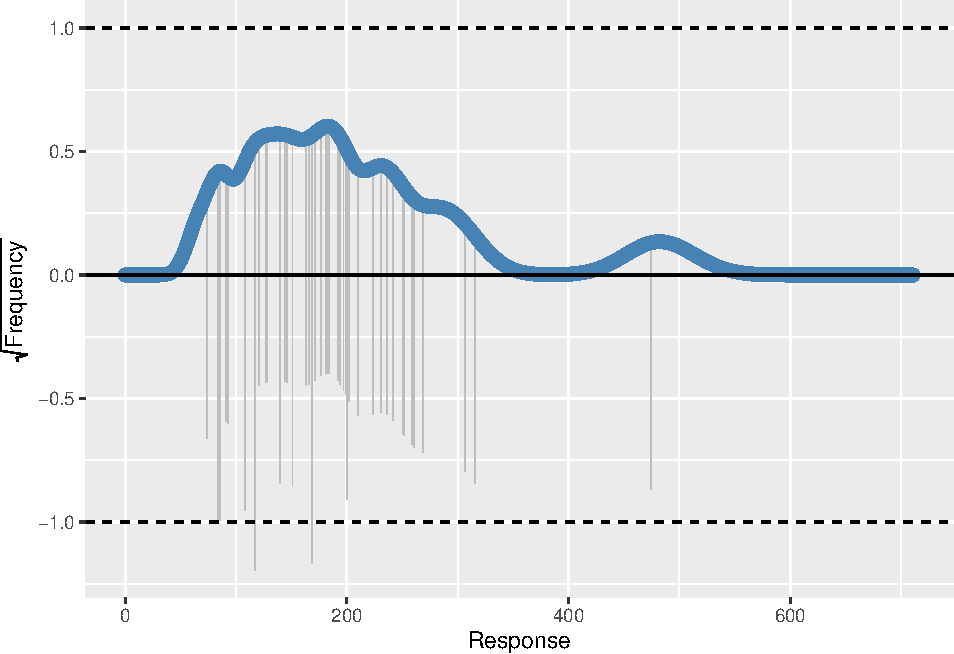
\includegraphics{Statistical-Analysis--Prediction-of-Trail-Use-in-Bridger-Mountains_files/figure-latex/rootogram-1.pdf}

Looking at Figure \ref{rootogram} we see the main features of the rootogram:

\begin{itemize}
\tightlist
\item
  expected counts, given the model, are shown by the thick blue line,
\item
  observed counts are shown as bars, which in a hanging rootogram are show hanging from the blue line of expected counts,
\item
  on the x-axis we have the count bin, 0 count, 1 count, 2 count, etc,
\item
  on the y-axis we have the square root of the observed or expected count --- the square root transformation allows for departures from expectations to be seen even at small frequencies,
\item
  a reference line is drawn at a height of 0.
\end{itemize}

Because this is a hanging rootogram, we can think of the rootogram as relating to the fitted counts --- if a bar doesn't reach the zero line then the model over predicts a particular count bin, and if the bar exceeds the zero line it under predicts.

\hypertarget{ACF}{%
\subsubsection{Identifying AR and MA using ACF and PACF Plots}\label{ACF}}

There are two visualizations of the residuals that can help you model autocorrelations: the ACF graph and the PACF. In general, ACF lets you assess the moving average component of the model and PACF lets you identify the autoregressive component. The p,q parameters can be estimated from the sharp cut off in the (P)ACF graphs.

\begin{Shaded}
\begin{Highlighting}[]
\FunctionTok{layout}\NormalTok{(}\FunctionTok{matrix}\NormalTok{(}\DecValTok{1}\SpecialCharTok{:}\DecValTok{2}\NormalTok{, }\AttributeTok{ncol =} \DecValTok{2}\NormalTok{))}
\FunctionTok{acf}\NormalTok{(}\FunctionTok{resid}\NormalTok{(gamm\_mod2}\SpecialCharTok{$}\NormalTok{lme, }\AttributeTok{type =} \StringTok{"normalized"}\NormalTok{), }
    \AttributeTok{lag.max =} \DecValTok{36}\NormalTok{, }\AttributeTok{main =} \StringTok{"ACF"}\NormalTok{)}
\FunctionTok{pacf}\NormalTok{(}\FunctionTok{resid}\NormalTok{(gamm\_mod2}\SpecialCharTok{$}\NormalTok{lme, }\AttributeTok{type =} \StringTok{"normalized"}\NormalTok{),}
     \AttributeTok{lag.max =} \DecValTok{36}\NormalTok{, }\AttributeTok{main =} \StringTok{"pACF"}\NormalTok{)}
\end{Highlighting}
\end{Shaded}

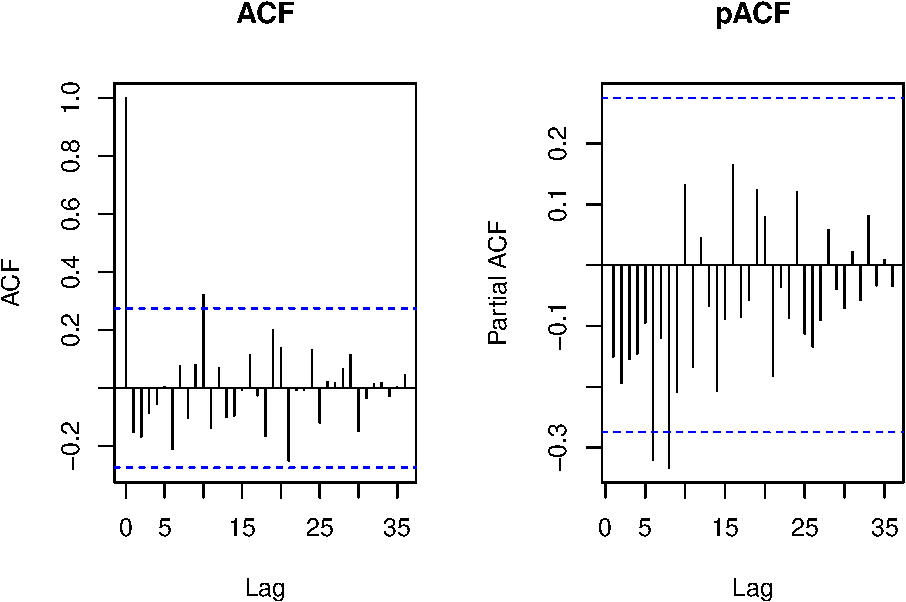
\includegraphics{Statistical-Analysis--Prediction-of-Trail-Use-in-Bridger-Mountains_files/figure-latex/gamm diagnostics-1.pdf}

\begin{Shaded}
\begin{Highlighting}[]
\FunctionTok{layout}\NormalTok{(}\DecValTok{1}\NormalTok{)}
\end{Highlighting}
\end{Shaded}

\hypertarget{choosing-an-appropriate-model-for-trail-use-in-middle-cottonwood}{%
\subsection{Choosing an Appropriate Model for Trail Use in Middle Cottonwood}\label{choosing-an-appropriate-model-for-trail-use-in-middle-cottonwood}}

Often when we fit a linear regression model, we use R-squared as a way to assess how well a model fits the data.

R-squared represents the proportion of the variance in the response variable that can be explained by the predictor variables in a regression model. This number ranges from 0 to 1, with higher values indicating a better model fit. However, there is no such R-squared value for general linear models like logistic regression models and Poisson regression models. Instead, we can calculate a metric known as McFadden's R-Squared, which ranges from 0 to just under 1, with higher values indicating a better model fit.

You shouldn't compare the AICs between objects fitted with different software. gam() is fitted via the mgcv package, whereas gamm() fit is actually accomplished via the MASS (glmmPQL()) and then nlme (lme()) packages. It would be common for different constants to end up in the log likelihood.

Within the \texttt{gamm} framework we may use \texttt{anova}() to compare between models with different temporal autocorrelation structures.

\begin{verbatim}
##                   Model df      AIC      BIC    logLik   Test  L.Ratio p-value
## gamm_mod2$lme         1 13 76.82418 101.9379 -25.41209                        
## gamm_mod2_AR1$lme     2 15 91.00384 119.9812 -30.50192 1 vs 2 10.17966  0.0062
\end{verbatim}

This output indicates that our \texttt{gamm\_mod2} fit (without any temporal correlation structure) is the best (i.e.~has the lowest AIC and BIC values).

\begin{tabular}{lrr}
\toprule
model & AIC & R.sq\\
\midrule
lm\_mod & 571.6371 & 0.31\\
glm\_mod & 1192.8703 & 0.41\\
gam\_mod & 784.5881 & 0.64\\
gamm\_mod & NA & 0.64\\
gamm\_mod2 & NA & 0.90\\
\addlinespace
gamm\_AR1 & NA & 0.83\\
\bottomrule
\end{tabular}

\textbf{Final Choice: Generalized Additive Mixture Model with Explanatory Variables}

\hypertarget{MidCotPred}{%
\section{Prediction and Forecasting Trail Use}\label{MidCotPred}}

A common issue with any model, the generalized additive modelling framework included, is how to extrapolate beyond the range of data used to train the model. Temporal extrapolation is particularly tricky with temporal (time series) data. For GAMs, the issue arises as this framework uses splines to learn from the data via the basis functions. The splines are often set up directly related to the data included in the training set and it's not always clear how these should extend past that range of data, especially in this single trail application. (In Section \ref{AllTrailsAnalysis} we apply this framework to a suite of trails and allow for a global smoother which can help inform trails with shorter camera deployment times by pulling/sharing from these global trends.)

Figure \ref{fig:MidCot-predict-compare} shows predictions (and 95\% credible interval on predicted values) for three different model specifications (\texttt{gam} with no temporal autocorrelation structure, \texttt{gamm} with no temporal autocorrelation structure, and \texttt{gamm} with an AR1 temporal autocorrelation structure). It's clear that all models perform best when interpolating, as expected. Improving forecasting with this single trail approach could be accomplished with several years of year-round observations.

\begin{figure}

{\centering 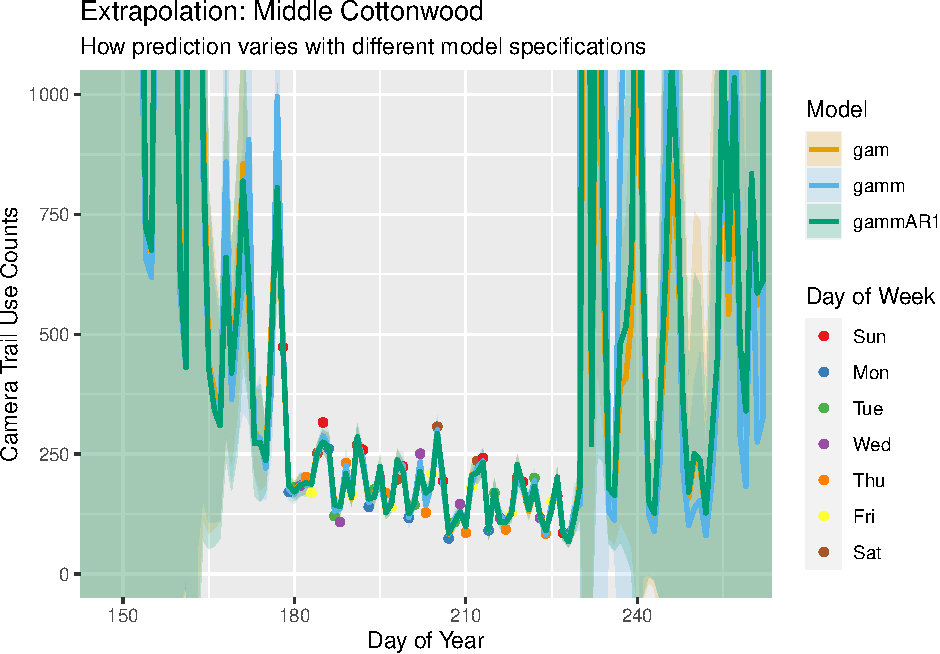
\includegraphics{Statistical-Analysis--Prediction-of-Trail-Use-in-Bridger-Mountains_files/figure-latex/MidCot-predict-compare-1} 

}

\caption{Predictions for Middle Cottonwood trail use showing interpolation and extrapolation behavior for temporal data range and extrended one month before and after data availability. Data points are colored by day of the week. Prediction lines (and error ribbons) are colored by model type applied.}\label{fig:MidCot-predict-compare}
\end{figure}

\hypertarget{AllTrailsAnalysis}{%
\chapter{Analysis of All Trails}\label{AllTrailsAnalysis}}

\hypertarget{data-used-1}{%
\section{Data Used}\label{data-used-1}}

This joint analysis covers the following Bridger Mountain subtrails:

\begin{enumerate}
\def\labelenumi{\arabic{enumi}.}
\tightlist
\item
  Fairy Creek
\item
  College M
\item
  Bridger
\item
  Steep Way
\item
  Sacagawea Pass
\item
  Carroll Creek
\item
  Raptor View
\item
  Sypes Canyon
\item
  College M to Sypes
\item
  Truman Gulch
\item
  East Bridger South
\item
  East Bridger North
\item
  Lower Shafthouse
\item
  Corbly Gulch
\item
  North Cottonwood to Johnson Canyon
\item
  North Cottonwood Access
\item
  Ross Pass
\item
  Middle Cottonwood
\item
  Johnson Canyon Jeep Trail
\item
  Benchmark Road
\item
  Horsethief Mountain
\end{enumerate}

\hypertarget{fitting-a-generalized-additive-mixture-model}{%
\section{Fitting a Generalized Additive Mixture Model}\label{fitting-a-generalized-additive-mixture-model}}

Here, we extend the Generalized Additive (Mixture) Model we first explained in Section \ref{Models} and then examined through application to Middle Cottonwood trail in Section \ref{MidCot} to now include all Bridger trails with counter camera data. This extension now includes different grouping levels (trail subsections) that require modeling of nonlinear functional relationships between covariates and outcomes where the shape of the function itself varies between different grouping levels. Hierarchical GA(M)Ms provide a natural extension to the standard GAM framework that allows smooth functional relationships between predictor and response to vary between groups, but in such a way that the different functions are in some sense pooled toward a common shape.

All models are fit in R. HGAMs are fit with the \textbf{mgcv} package \citep[\citet{R-Wood2}, \citet{R-Wood3}, \citet{R-Wood4}, \citet{R-Wood5}]{R-Wood1}.

In our application, where we want to estimate and predict trail use at trails in the Bridger Mountains, we may assume that each trail will have its own response function (e.g.~melting snowpack may take longer at higher elevation and thus trail use would be concentrated on trails that clear sooner), but since the trails are all in the same range we can also expect similar responses over the year. Estimating a separate function for each trail (or subsection) throws away a lot of shared information and could result in highly noisy function estimates if there were only a few data points for some trails. Conversely, estimating a single average relationship could result in a function that does not predict any specific group well. We aimed for a hierarchical model that includes a global curve plus trail subsection-specific curves that were penalized to be close to the mean function.

Sometimes this dependence can be capture using the fixed and random effects in a GAMM, however when modelling all trails in this dataset we observed remaining temporal dependence (not shown, but see the ACF and PACF graph explanations in Section \ref{ACF} for an overview of how to diagnose this dependence). For each model we examine three possible temporal autocorrelation structures: none, AR1, and ARMA. Summary and diagnostic plots are only presented for the best model.

\hypertarget{accounting-for-trailsubsection-grouping}{%
\subsection{Accounting for Trail/Subsection Grouping}\label{accounting-for-trailsubsection-grouping}}

A key feature of these data that we need to account for in our model is the random effect of trail, and for some trails the different subsections. Both \texttt{gam} and \texttt{gamm} in the \textbf{mgcv} package can incorporate random effects through a smoothing term that, in R, would look similar to

\begin{Shaded}
\begin{Highlighting}[]
\NormalTok{re\_mod }\OtherTok{\textless{}{-}} \FunctionTok{gam}\NormalTok{(response }\SpecialCharTok{\textasciitilde{}}\NormalTok{ maineffect }\SpecialCharTok{+}
                \FunctionTok{s}\NormalTok{(randomeffect, }\AttributeTok{bs =} \StringTok{\textquotesingle{}re\textquotesingle{}}\NormalTok{),}
              \AttributeTok{data =}\NormalTok{ data,}
              \AttributeTok{method =} \StringTok{\textquotesingle{}REML\textquotesingle{}}\NormalTok{)}
\end{Highlighting}
\end{Shaded}

Note that the random effect is denoted with \texttt{bs="re"}. Multiple random effects would each have its own smoothing term in the model. Another key requirement of this application is that the random effect term must be coded as a factor term. These random effect terms are adding random intercepts (deviations from the overall mean, the model constant term) for each level of the factors.

\hypertarget{global-smoothing-model-g}{%
\subsection{Global Smoothing Model (G)}\label{global-smoothing-model-g}}

We start with a simple GAMM structure with a single smooth for each of the variables.

In R we can write our model as:

\begin{Shaded}
\begin{Highlighting}[]
\NormalTok{gamm\_modG\_ARMA }\OtherTok{\textless{}{-}} \FunctionTok{gamm}\NormalTok{(max.camera }\SpecialCharTok{\textasciitilde{}}
                         \FunctionTok{s}\NormalTok{(yday, }\AttributeTok{bs=}\StringTok{"tp"}\NormalTok{) }\SpecialCharTok{+}
                         \FunctionTok{s}\NormalTok{(subsectionF, }\AttributeTok{bs=}\StringTok{"re"}\NormalTok{, }\AttributeTok{k=}\DecValTok{21}\NormalTok{) }\SpecialCharTok{+}
                         \FunctionTok{s}\NormalTok{(month, }\AttributeTok{bs=}\StringTok{"tp"} \AttributeTok{k =} \DecValTok{7}\NormalTok{) }\SpecialCharTok{+}
                         \FunctionTok{s}\NormalTok{(wday, }\AttributeTok{bs =} \StringTok{"cc"}\NormalTok{, }\AttributeTok{k =} \DecValTok{7}\NormalTok{) }\SpecialCharTok{+}
                         \FunctionTok{s}\NormalTok{(daily\_aqi\_value, }\AttributeTok{bs=}\StringTok{"tp"}\NormalTok{, }\AttributeTok{k =} \DecValTok{10}\NormalTok{) }\SpecialCharTok{+}
                         \FunctionTok{s}\NormalTok{(temp\_max\_f, }\AttributeTok{bs=}\StringTok{"tp"}\NormalTok{, }\AttributeTok{k =} \DecValTok{10}\NormalTok{) }\SpecialCharTok{+}
                         \FunctionTok{s}\NormalTok{(precipitation\_in, }\AttributeTok{bs =} \StringTok{"tp"}\NormalTok{, }\AttributeTok{k =} \DecValTok{5}\NormalTok{) }\SpecialCharTok{+}
                        \FunctionTok{s}\NormalTok{(totallength\_miles,  }\AttributeTok{bs=}\StringTok{"tp"}\NormalTok{, }\AttributeTok{k =} \DecValTok{10}\NormalTok{) }\SpecialCharTok{+} 
\NormalTok{                        total\_traveltime }\SpecialCharTok{+}
\NormalTok{                         max.count}
\NormalTok{                        ,}
                      \AttributeTok{method =} \StringTok{\textquotesingle{}REML\textquotesingle{}}\NormalTok{,}
                       \AttributeTok{data =}\NormalTok{ allTrail, }
                      \AttributeTok{correlation =} \FunctionTok{corARMA}\NormalTok{(}\AttributeTok{form =} \SpecialCharTok{\textasciitilde{}}\NormalTok{yday}\SpecialCharTok{|}\NormalTok{subsectionF,}
                                            \AttributeTok{p =} \DecValTok{1}\NormalTok{, }\AttributeTok{q =} \DecValTok{2}\NormalTok{),}
                      \AttributeTok{family =}\NormalTok{ poisson, }
                      \AttributeTok{niterPQL =} \DecValTok{20}\NormalTok{)}
\end{Highlighting}
\end{Shaded}

The arguments to the s() terms are smoothed. For each we explicitly specify the type of smoother to be used with the bs argument, and the maximum number of basis functions with k. The default type of smoother is the TPRS smoother (``tp'') and the default value for k (for TPRS) is 10. We use a cyclic cubic spline (``cc'') for day of week (wday) and set k=7 as we have seven unique values in this variable. We also set k=7 for month for the same reason; the data spans seven months of the year. If camera counters are deployed year-round in the future we would use bs=``cc'' and k=12 for this variable. The random effect smoother (bs=``re'') that we used for the subsectionF factor always has a k value equal to the number of levels in the grouping variable (here, 21). We restrict the number of knots for \texttt{precipitation\_in} (k=5) to curb some weird behavior likely due to very few non-zero values.

For each model (G, GS, GI) we will use the \textbf{forecast} package to determine the optimum values of \(p\) and \(q\) in the ARMA correlation structure, but, for brevity, won't always report this outcome.

\begin{Shaded}
\begin{Highlighting}[]
\DocumentationTok{\#\# this should help find values for p and q in the ARMA model }
\NormalTok{arma\_res\_G }\OtherTok{\textless{}{-}}\NormalTok{ forecast}\SpecialCharTok{::}\FunctionTok{auto.arima}\NormalTok{(}\FunctionTok{resid}\NormalTok{(gamm\_modG}\SpecialCharTok{$}\NormalTok{lme, }\AttributeTok{type =} \StringTok{"normalized"}\NormalTok{), }
                                   \AttributeTok{seasonal =}\NormalTok{ T)}
 
\NormalTok{arma\_res\_G}\SpecialCharTok{$}\NormalTok{coef}
\end{Highlighting}
\end{Shaded}

\begin{verbatim}
##        ar1        ar2        ma1 
##  1.1270770 -0.1848592 -0.7771053
\end{verbatim}

The summary and various diagnostic plots will only be shown for the ``best'' model (between the different correlation structures) as determined by anova. For model G, we will present the model with the ARMA correlation structure only.

\begin{verbatim}
##                    Model df      AIC      BIC    logLik   Test  L.Ratio p-value
## gamm_modG$lme          1 15 39089.53 39164.07 -19529.76                        
## gamm_modG_AR1$lme      2 16 33455.64 33535.16 -16711.82 1 vs 2 5635.882  <.0001
## gamm_modG_ARMA$lme     3 20 31217.28 31316.68 -15588.64 2 vs 3 2246.360  <.0001
\end{verbatim}

The summary output indicates that all of our included parametric (linear) coefficients and smooth terms are (approximately) significant. The effective degree of freedom (edf) values represents the complexity of the smooth. We can see in this output that the highest smooth complexity is for \texttt{subsectionF}. The adjusted R-sq value (which should not be employed as an absolute measure of model performance) is 0.78 for this model.

\begin{Shaded}
\begin{Highlighting}[]
\FunctionTok{summary}\NormalTok{(gamm\_modG\_ARMA}\SpecialCharTok{$}\NormalTok{gam)}
\end{Highlighting}
\end{Shaded}

\begin{verbatim}
## 
## Family: poisson 
## Link function: log 
## 
## Formula:
## max.camera ~ s(yday, bs = "cc") + s(subsectionF, bs = "re", k = sub.number) + 
##     s(month, k = 7) + s(wday, bs = "cc", k = 7) + s(daily_aqi_value) + 
##     s(temp_max_f) + s(precipitation_in, k = 5) + s(totallength_miles) + 
##     total_traveltime + max.count
## 
## Parametric coefficients:
##                    Estimate Std. Error t value Pr(>|t|)    
## (Intercept)       3.3383574  0.3398840   9.822  < 2e-16 ***
## total_traveltime -0.0256714  0.0095960  -2.675  0.00759 ** 
## max.count         0.0103780  0.0005349  19.401  < 2e-16 ***
## ---
## Signif. codes:  0 '***' 0.001 '**' 0.01 '*' 0.05 '.' 0.1 ' ' 1
## 
## Approximate significance of smooth terms:
##                         edf Ref.df       F  p-value    
## s(yday)               7.966  8.000 582.017  < 2e-16 ***
## s(subsectionF)       16.262 19.000  95.121  < 2e-16 ***
## s(month)              5.209  5.209  25.987  < 2e-16 ***
## s(wday)               4.984  5.000 627.438  < 2e-16 ***
## s(daily_aqi_value)    8.888  8.888 166.946  < 2e-16 ***
## s(temp_max_f)         8.747  8.747 878.221  < 2e-16 ***
## s(precipitation_in)   3.797  3.797  71.549  < 2e-16 ***
## s(totallength_miles)  2.491  2.491   8.491 0.000144 ***
## ---
## Signif. codes:  0 '***' 0.001 '**' 0.01 '*' 0.05 '.' 0.1 ' ' 1
## 
## R-sq.(adj) =  0.784   
##   Scale est. = 1         n = 1064
\end{verbatim}

In figures \ref{fig:modG-TSdiag1} and \ref{fig:modG-TSdiag2}, we examine several diagnostic plots for a time series GAMM fit. A more detailed explanation of all of these plots and how to interpret them is available in Section \ref{Diag}. We are not looking for a perfect fit with this model, rather including these diagnostic plots so that they may be compared to those from fitting the data to models GS and GI.

\begin{figure}

{\centering 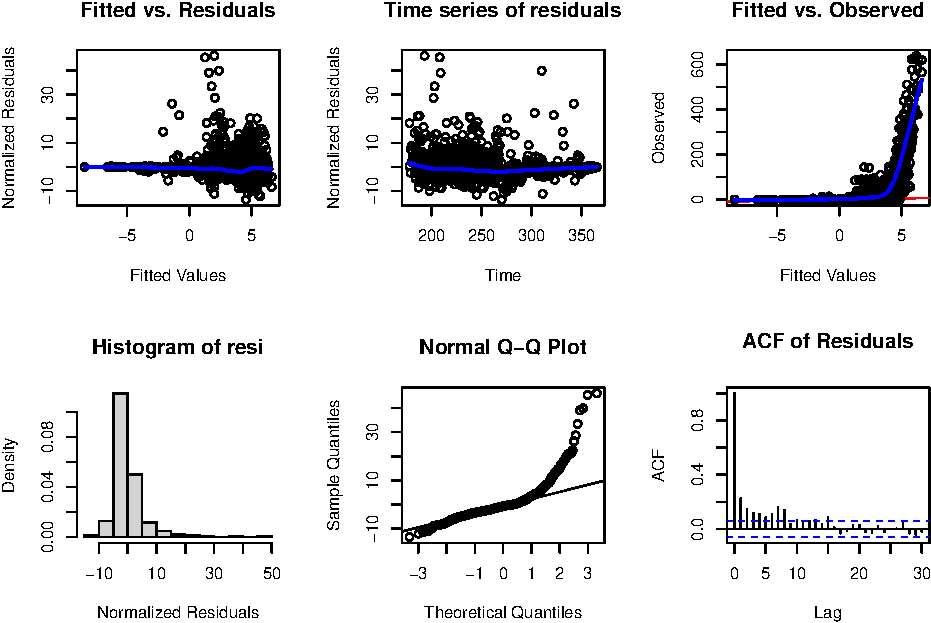
\includegraphics[width=1\linewidth]{Statistical-Analysis--Prediction-of-Trail-Use-in-Bridger-Mountains_files/figure-latex/modG-TSdiag1-1} 

}

\caption{GAMM time series   diagnostic plots for model \emph{G}.}\label{fig:modG-TSdiag1}
\end{figure}

\begin{figure}

{\centering 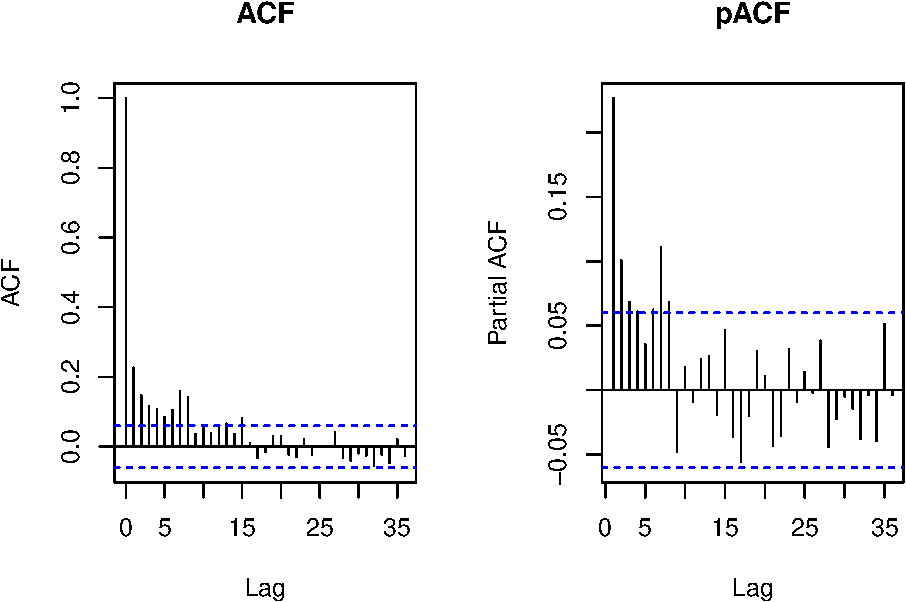
\includegraphics[width=1\linewidth]{Statistical-Analysis--Prediction-of-Trail-Use-in-Bridger-Mountains_files/figure-latex/modG-TSdiag2-1} 

}

\caption{ACF/pACF diagnostic plots for model \emph{G}.}\label{fig:modG-TSdiag2}
\end{figure}

Figure \ref{fig:modG-draw} partial effects plots for model G with an ARMA(1,2) temporal correlation structure. Partial effects are the isolated effects of one particular predictor or interaction of predictors. The output now includes a QQ-plot for the random effects term, showing the estimated intercepts for the different levels of \texttt{subsectionF}.

\begin{Shaded}
\begin{Highlighting}[]
\NormalTok{gratia}\SpecialCharTok{::}\FunctionTok{draw}\NormalTok{(gamm\_modG\_ARMA}\SpecialCharTok{$}\NormalTok{gam, }\AttributeTok{residuals =}\NormalTok{ F)}
\end{Highlighting}
\end{Shaded}

\begin{figure}
\centering
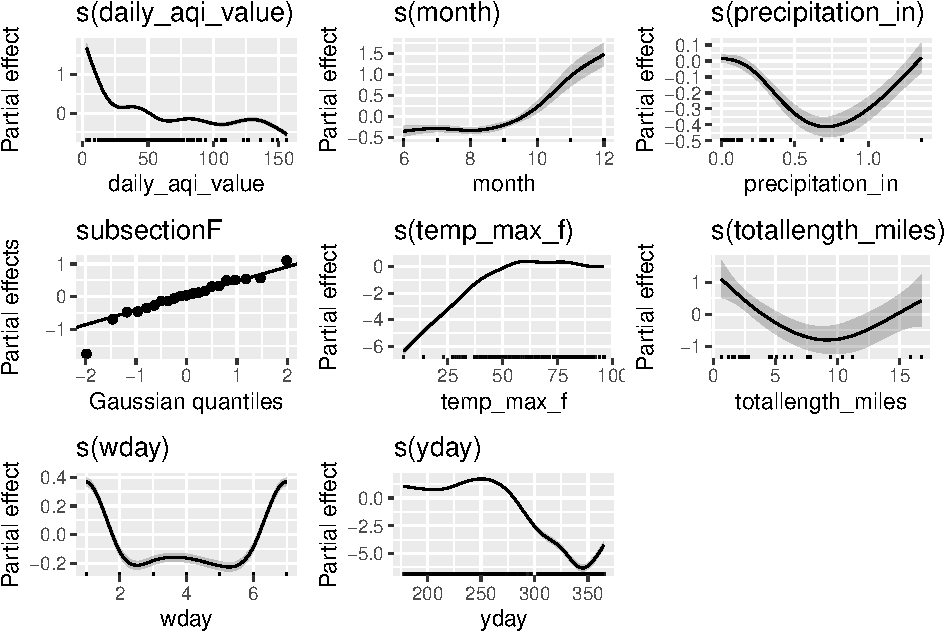
\includegraphics{Statistical-Analysis--Prediction-of-Trail-Use-in-Bridger-Mountains_files/figure-latex/modG-draw-1.pdf}
\caption{\label{fig:modG-draw}Partial effects plots for model \emph{G}.}
\end{figure}

The rootogram plot in Figure \ref{fig:modG-rootogram} shows that the data are slightly overdispersed (the variance, which is expected to be the same as the mean, is larger). Overdispersion for a poisson family distribution is not uncommon in real world data. Alternative families may be specified in the \texttt{gamm} code through the family argument, such as quasipoisson, negative binomial or (for \texttt{gam} only) a zero-inflated poisson family. Several alternatives were explored (not shown) but none provided improvements in overdisperson.

\begin{Shaded}
\begin{Highlighting}[]
\NormalTok{rg }\OtherTok{\textless{}{-}}\NormalTok{ gratia}\SpecialCharTok{::}\FunctionTok{rootogram}\NormalTok{(gamm\_modG\_ARMA}\SpecialCharTok{$}\NormalTok{gam)}
\FunctionTok{draw}\NormalTok{(rg)}
\end{Highlighting}
\end{Shaded}

\begin{figure}

{\centering 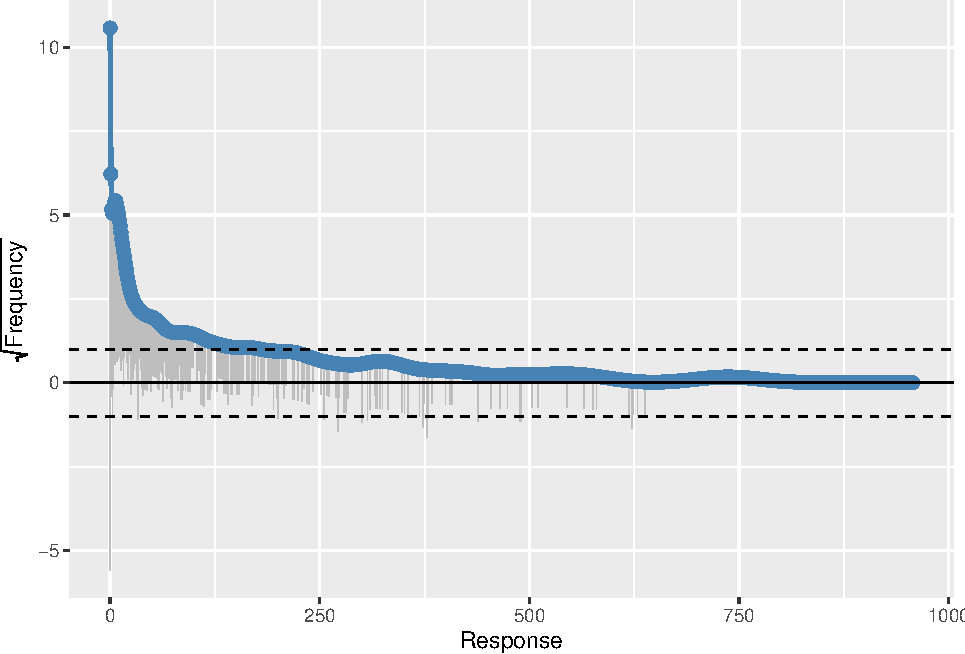
\includegraphics{Statistical-Analysis--Prediction-of-Trail-Use-in-Bridger-Mountains_files/figure-latex/modG-rootogram-1} 

}

\caption{Rootogram for checking for overdispersion.}\label{fig:modG-rootogram}
\end{figure}

Averaging over all of the variation (between trails) results in a relatively imprecise (diffuse) estimates of trail use (Figures \ref{fig:high-pred-G} and \ref{fig:low-pred-G}), and viewing species-specific plots of observed vs.~predicted values (Figure \ref{fig:modG-pred-observed}), it is apparent that the model fits some of the trail sections better than others. This model could potentially be improved by adding intergroup variation between trail subsections.

\begin{figure}

{\centering 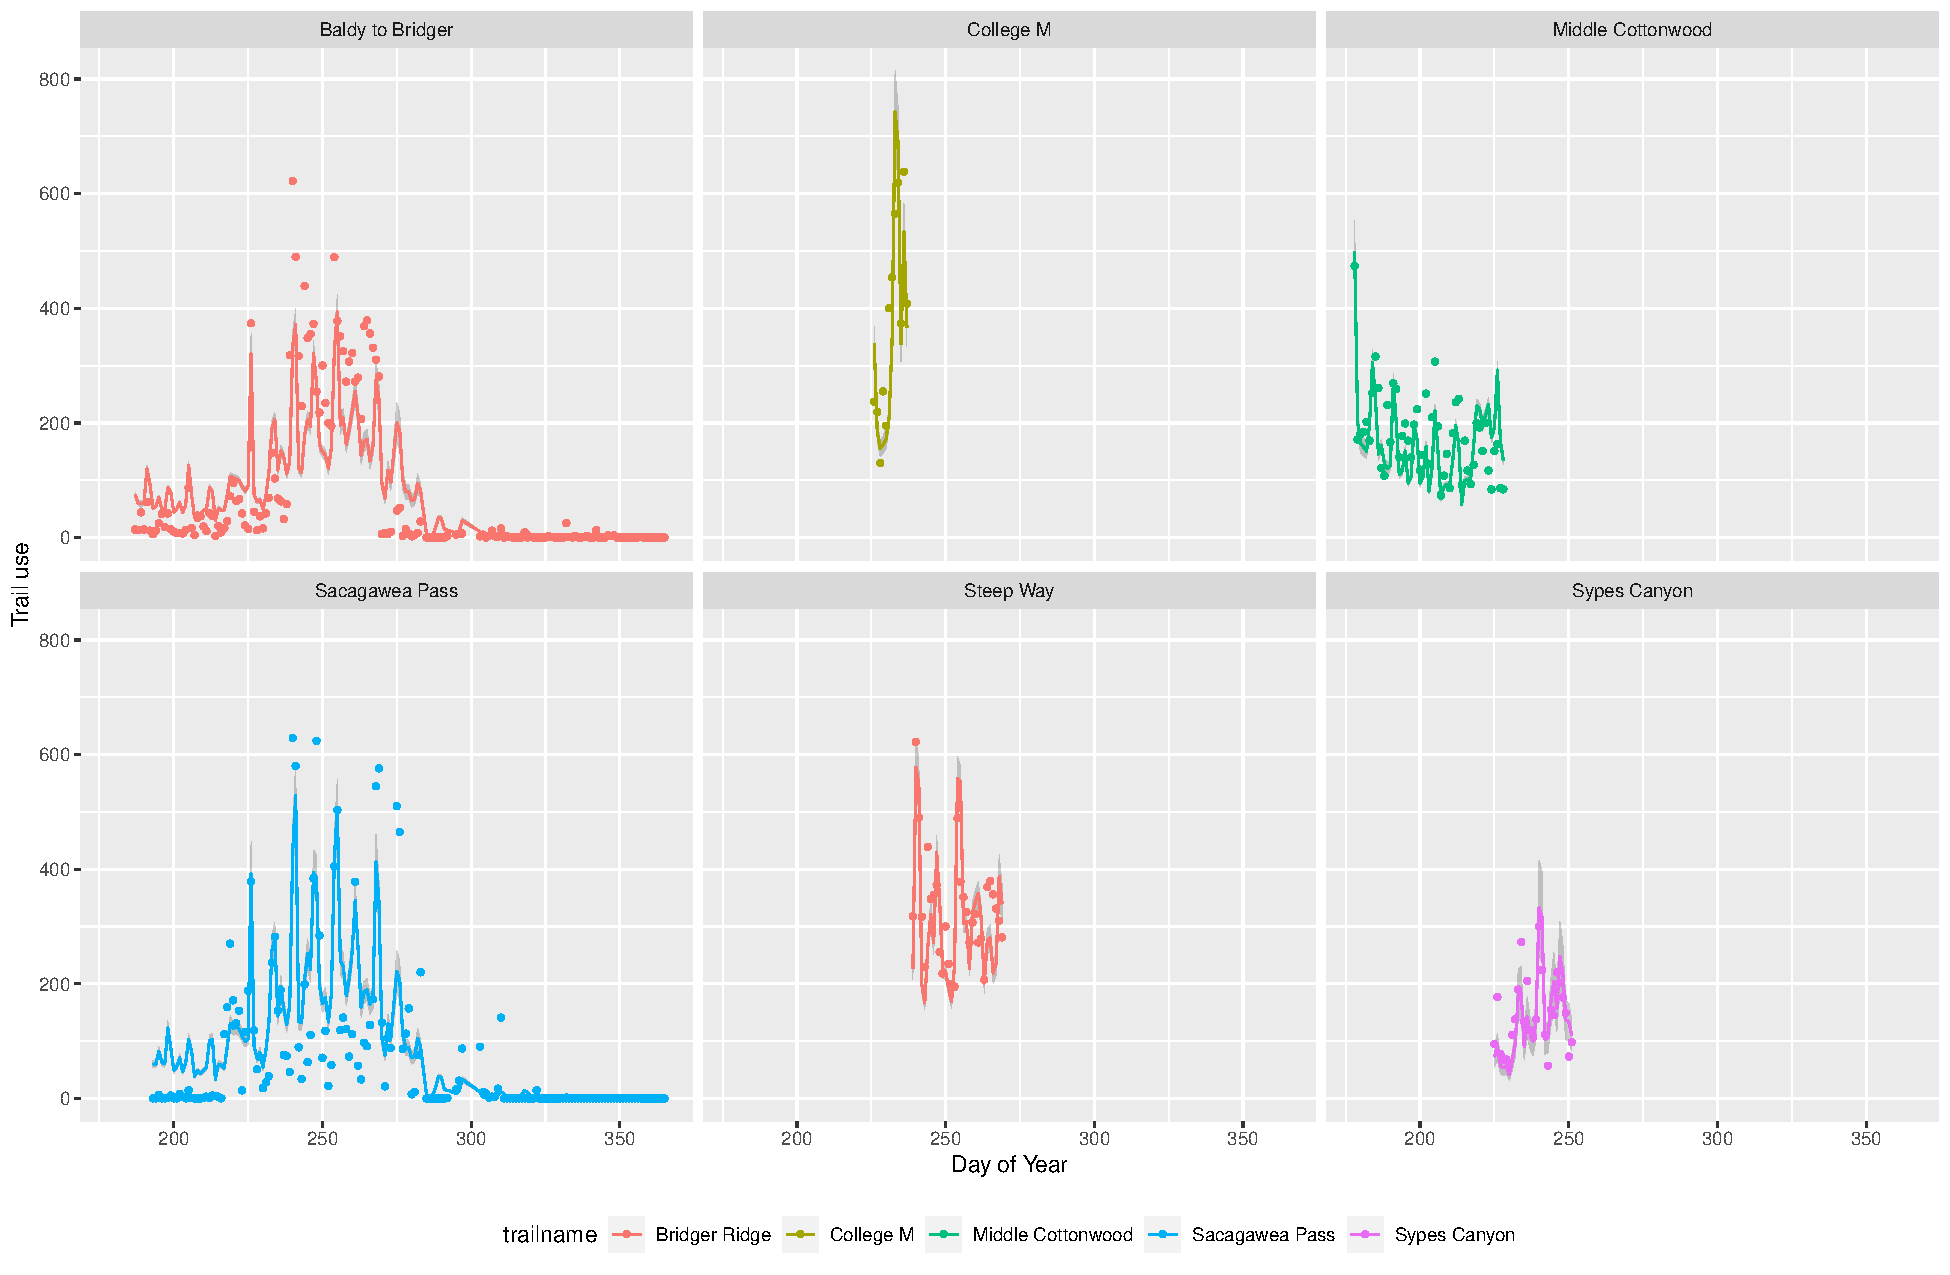
\includegraphics[width=1\linewidth]{../figures/high_pred_modG} 

}

\caption{Predicted trail use count values (lines) versus observed trail use (points) for each high-use trail subsection, based on model \emph{G}.}\label{fig:high-pred-G}
\end{figure}

\begin{figure}

{\centering 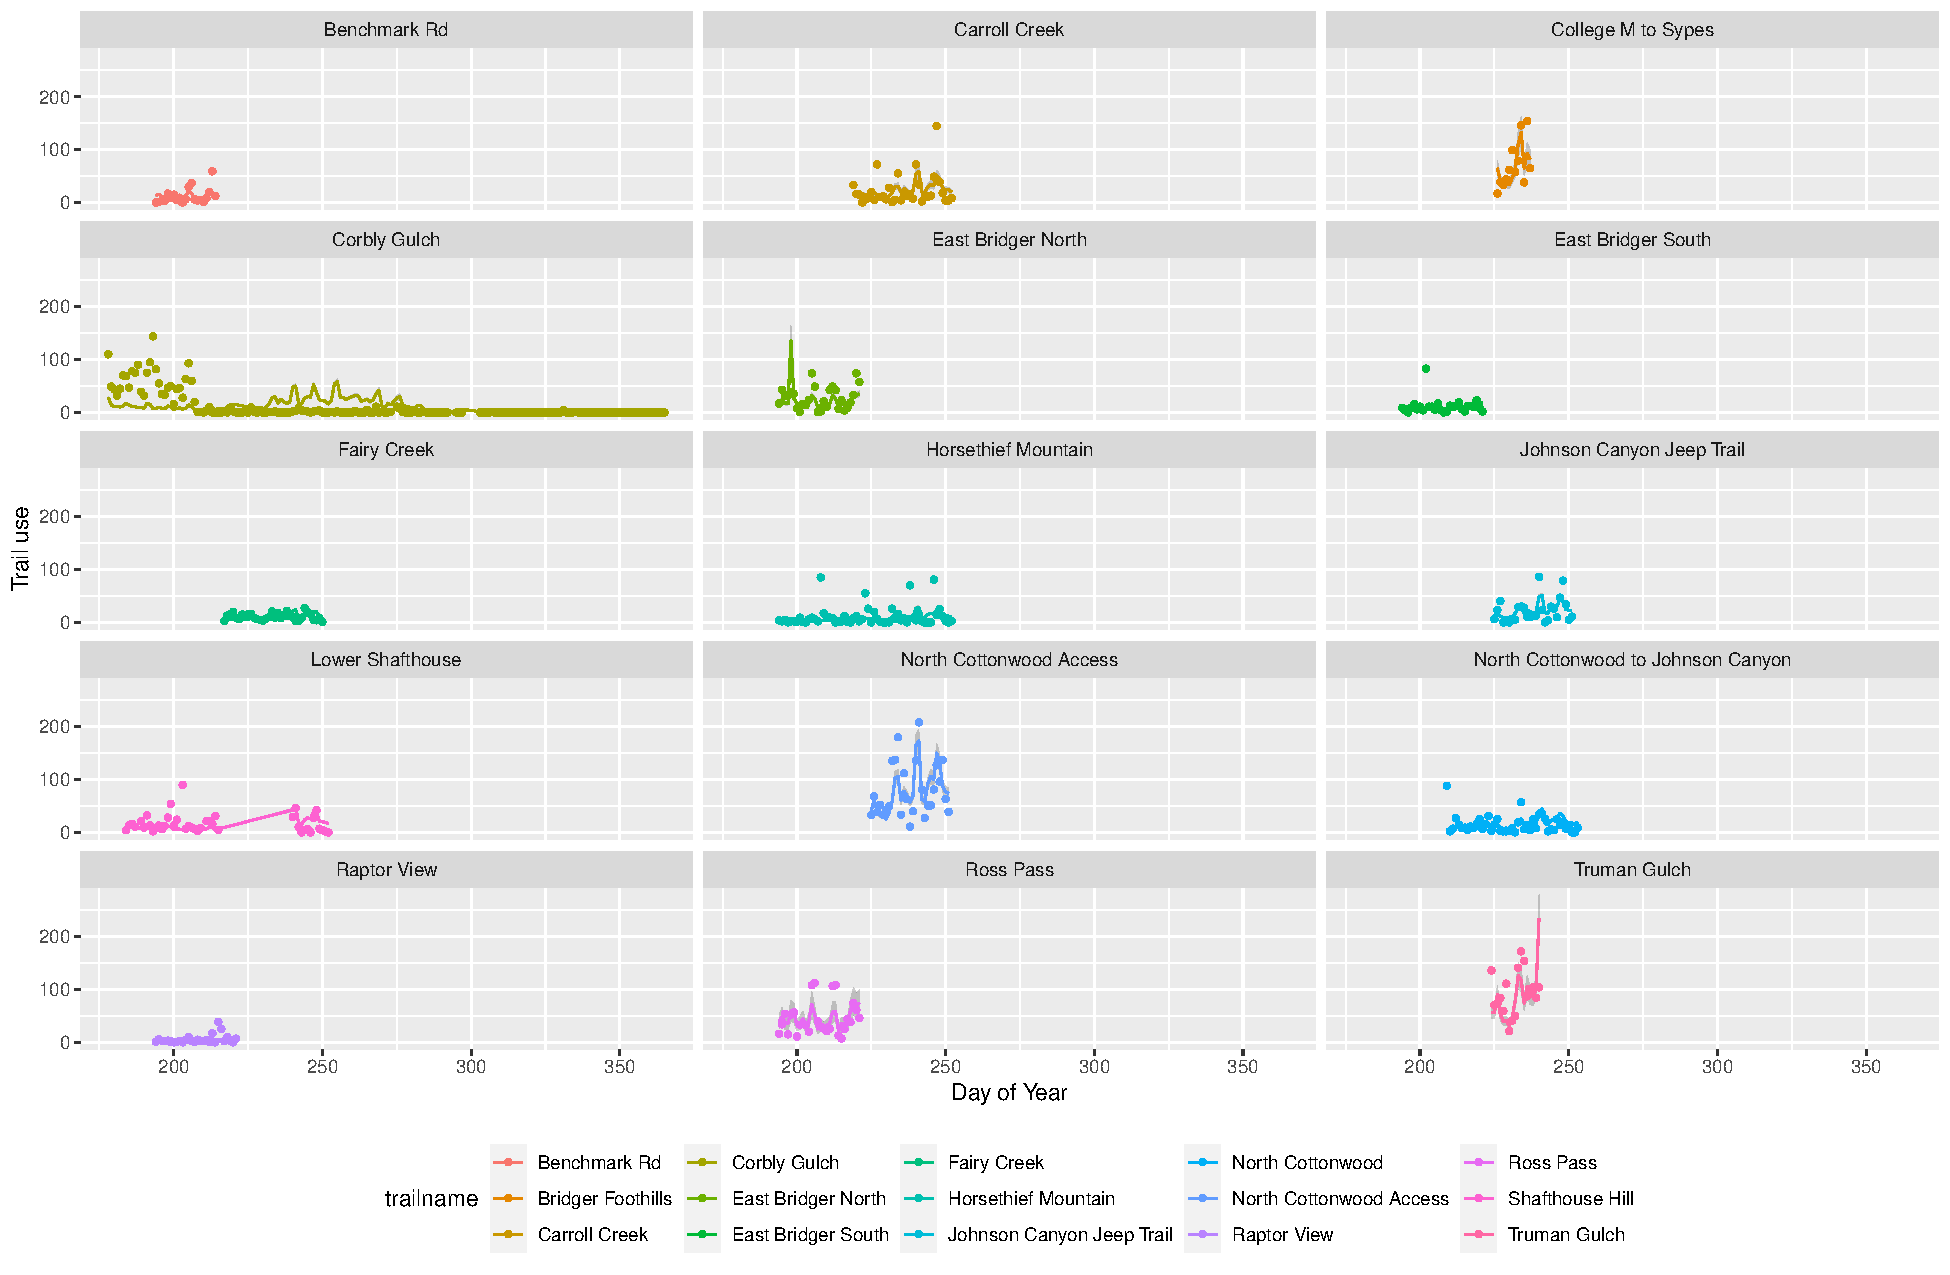
\includegraphics[width=1\linewidth]{../figures/low_pred_modG} 

}

\caption{Predicted trail use count values (lines) versus observed trail use (points) for each low-use trail subsection, based on model \emph{G}.}\label{fig:low-pred-G}
\end{figure}

Model GS is able to effectively capture the obseved pattern of trial use variation between trail subsections and shows slightly less evidence of overdispersion (Figure \ref{fig:modGS-pred-observed}) in some trail subsections compared to Model G (note the difference in Corbly Gulch).

\begin{Shaded}
\begin{Highlighting}[]
\CommentTok{\#add the predicted values from the model }
\NormalTok{allTrail\_G\_pred }\OtherTok{\textless{}{-}} \FunctionTok{transform}\NormalTok{(allTrail\_G, }
                      \AttributeTok{mod\_G =} \FunctionTok{predict}\NormalTok{(gamm\_modG\_ARMA}\SpecialCharTok{$}\NormalTok{gam, }
                                      \AttributeTok{type =} \StringTok{"response"}\NormalTok{))}

\FunctionTok{ggplot}\NormalTok{(allTrail\_G\_pred, }\FunctionTok{aes}\NormalTok{(}\AttributeTok{x=}\NormalTok{mod\_G, }\AttributeTok{y=}\NormalTok{max.camera)) }\SpecialCharTok{+}
  \FunctionTok{facet\_wrap}\NormalTok{(}\SpecialCharTok{\textasciitilde{}}\NormalTok{subsectionF, }\AttributeTok{ncol=} \DecValTok{3}\NormalTok{) }\SpecialCharTok{+}
  \FunctionTok{geom\_point}\NormalTok{(}\AttributeTok{alpha=}\FloatTok{0.3}\NormalTok{, }\FunctionTok{aes}\NormalTok{(}\AttributeTok{color =}\NormalTok{ trailname)) }\SpecialCharTok{+}
  \FunctionTok{scale\_color\_manual}\NormalTok{(}\AttributeTok{name =} \StringTok{"Trail"}\NormalTok{, }\AttributeTok{values =}\NormalTok{ colors) }\SpecialCharTok{+}
  \FunctionTok{geom\_abline}\NormalTok{() }\SpecialCharTok{+}
  \FunctionTok{theme}\NormalTok{(}\AttributeTok{legend.position=}\StringTok{"none"}\NormalTok{) }\SpecialCharTok{+}
  \FunctionTok{labs}\NormalTok{(}\AttributeTok{x=}\StringTok{"Predicted count"}\NormalTok{, }\AttributeTok{y=}\StringTok{"Observed count"}\NormalTok{)}
\end{Highlighting}
\end{Shaded}

\begin{figure}

{\centering 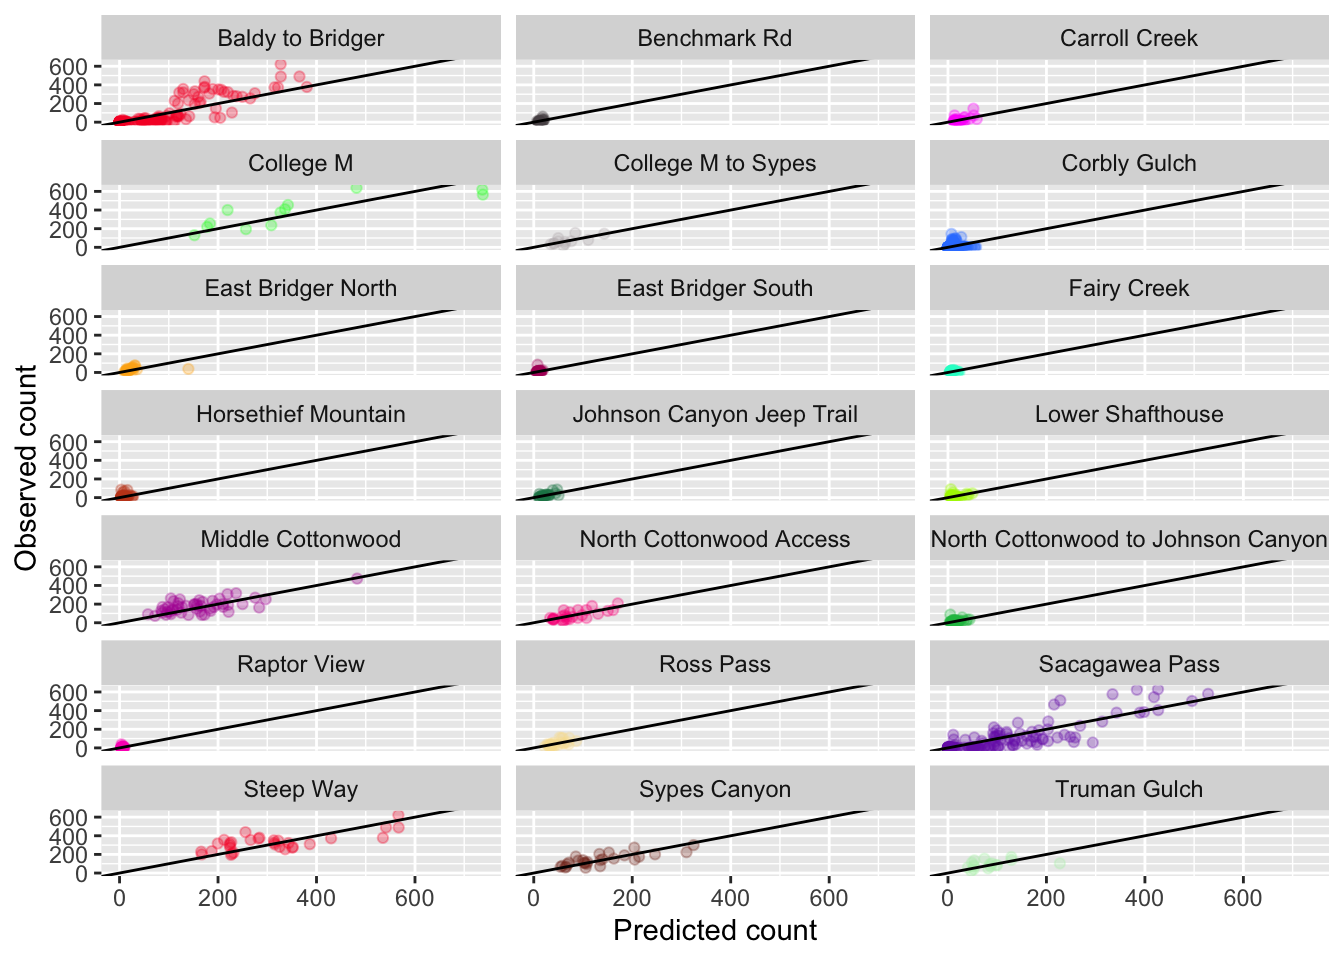
\includegraphics[width=1\linewidth]{Statistical-Analysis--Prediction-of-Trail-Use-in-Bridger-Mountains_files/figure-latex/modG-pred-observed-1} 

}

\caption{Assuming a well-fitted model G, we would expect all trail subsections exhibiting similar patterns of dispersion around the 1-1 line (and as we are assuming the data is Poisson, the variance around the mean should equal the mean). Instead we see that variance around the predicted value is much higher for some trails such as Sacagawea Pass.}\label{fig:modG-pred-observed}
\end{figure}

\hypertarget{single-common-smoother-plus-group-level-smoothers-that-have-the-same-wiggliness-model-gs}{%
\subsection{Single common smoother plus group-level smoothers that have the same wiggliness (model GS)}\label{single-common-smoother-plus-group-level-smoothers-that-have-the-same-wiggliness-model-gs}}

Model GS constricts all groups to having similar functional responses, but, unlike model G, intergroup variation in responses is allowed. This approach works by allowing each grouping level (here, \texttt{subsectionF}) to have its own functional response, but penalizing functions that are too far from the average.

In R we can write our model as:

\begin{Shaded}
\begin{Highlighting}[]
\NormalTok{ gamm\_modGS\_AR1 }\OtherTok{\textless{}{-}} \FunctionTok{gamm}\NormalTok{(max.camera }\SpecialCharTok{\textasciitilde{}} 
                           \FunctionTok{s}\NormalTok{(yday, }\AttributeTok{m=}\DecValTok{2}\NormalTok{, }\AttributeTok{bs=}\StringTok{"cc"}\NormalTok{) }\SpecialCharTok{+}
                           \FunctionTok{s}\NormalTok{(yday, subsectionF,}
                             \AttributeTok{m=}\DecValTok{2}\NormalTok{, }\AttributeTok{bs=}\StringTok{"fs"}\NormalTok{, }\AttributeTok{k =} \DecValTok{21}\NormalTok{) }\SpecialCharTok{+}
                           \CommentTok{\# s(subsectionF, bs = "re", k= 21) +}
                           \FunctionTok{s}\NormalTok{(month, }\AttributeTok{bs =} \StringTok{"cc"}\NormalTok{, }\AttributeTok{k =} \DecValTok{7}\NormalTok{) }\SpecialCharTok{+}
                           \FunctionTok{s}\NormalTok{(wday,}
                             \AttributeTok{bs =} \StringTok{"cc"}\NormalTok{, }\AttributeTok{k =} \DecValTok{7}\NormalTok{) }\SpecialCharTok{+}
                           \FunctionTok{s}\NormalTok{(daily\_aqi\_value) }\SpecialCharTok{+}
                           \FunctionTok{s}\NormalTok{(temp\_max\_f) }\SpecialCharTok{+}
                           \FunctionTok{s}\NormalTok{(precipitation\_in, }\AttributeTok{k =} \DecValTok{5}\NormalTok{) }\SpecialCharTok{+}
                          \FunctionTok{s}\NormalTok{(totallength\_miles) }\SpecialCharTok{+} 
\NormalTok{                        total\_traveltime }\SpecialCharTok{+}
\NormalTok{                            max.count,}
                          \AttributeTok{knots =} \FunctionTok{list}\NormalTok{(}\AttributeTok{yday =} \FunctionTok{c}\NormalTok{(}\DecValTok{0}\NormalTok{,}\DecValTok{365}\NormalTok{),}
                                       \AttributeTok{month =} \FunctionTok{c}\NormalTok{(}\DecValTok{0}\NormalTok{, }\DecValTok{13}\NormalTok{)),}
                         \AttributeTok{data =}\NormalTok{ allTrail, }
                         \AttributeTok{method =} \StringTok{"REML"}\NormalTok{, }
                         \AttributeTok{correlation =} \FunctionTok{corAR1}\NormalTok{(}\AttributeTok{form =} \SpecialCharTok{\textasciitilde{}}\NormalTok{yday}\SpecialCharTok{|}\NormalTok{subsectionF),}
                         \AttributeTok{family =}\NormalTok{ poisson)}
\end{Highlighting}
\end{Shaded}

With this model specification we explicitly specifying one term for the global smoother (as in model G, above) then added a second smooth term specifying the group-level smooth terms (here, \texttt{subsectionF}), using a penalty term that tends to draw these group-level smoothers toward zero. This penalty is incorporated via the factor-smoothing basis type (\texttt{bs\ =\ "fs"}) which creates a copy of each set of basis functions for each level of the grouping variable, but only estimates one smoothing parameter for all groups (see \texttt{?mgcv::factor.smooth.interaction} for details).

Model GS with an ARMA correlation structure has been selected, but the summary does not seem to work on this model fit object. However, all other diagnostic plots and predictions work.

Diagnostic plots for time series data show there still is temporal autocorrelation left in the model.

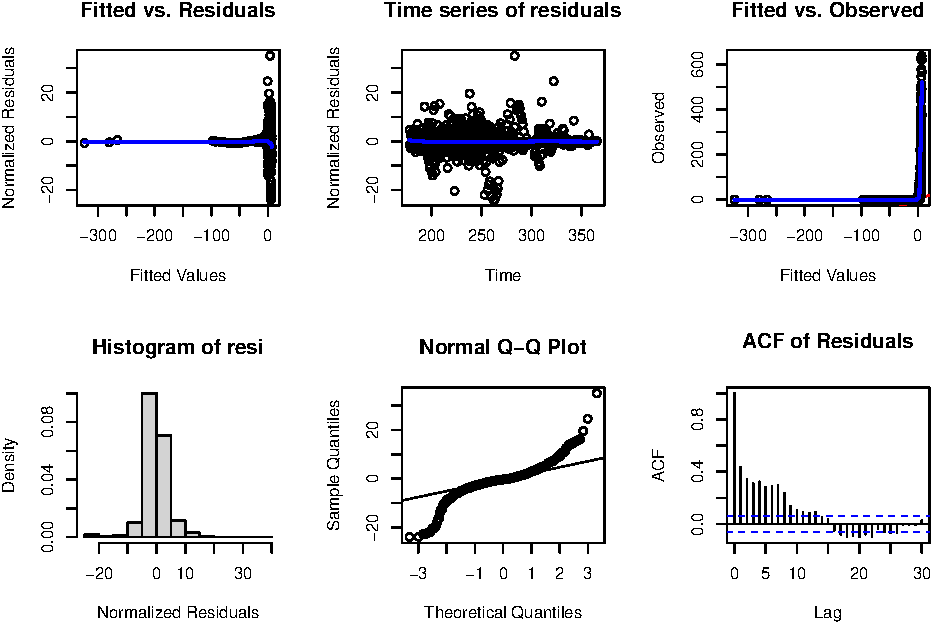
\includegraphics{Statistical-Analysis--Prediction-of-Trail-Use-in-Bridger-Mountains_files/figure-latex/modGS-tsDiag-1.pdf} 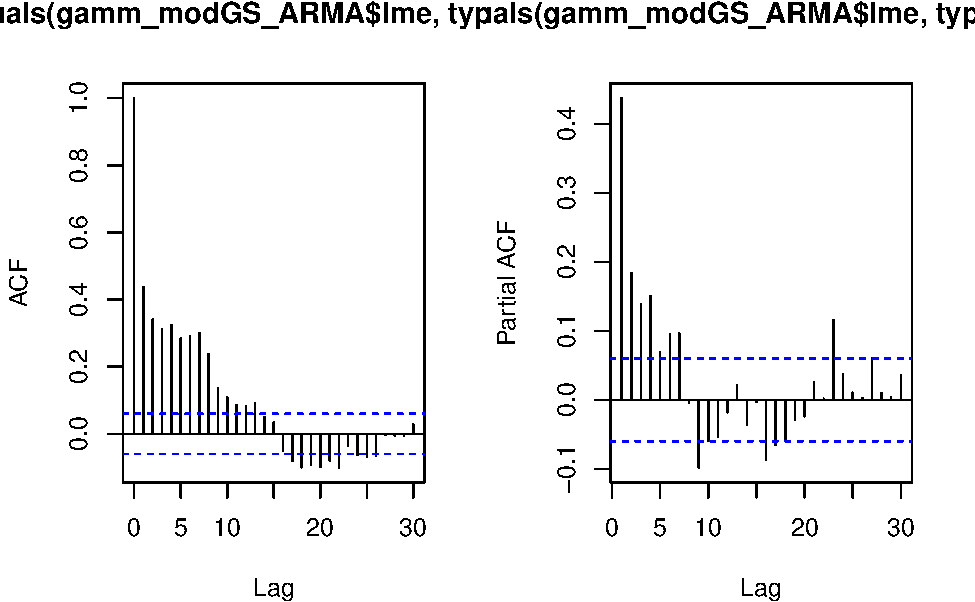
\includegraphics{Statistical-Analysis--Prediction-of-Trail-Use-in-Bridger-Mountains_files/figure-latex/modGS-tsDiag-2.pdf}

Figure \ref{fig:modelGS-draw} shows the fitted smoothers for \texttt{gamm\_modGS\_ARMA\_sub}. The plots of group-specific smoothers (bottom left) indicate that trail subsections differ not only in average (log) trail use (which would correspond to each trail having a straight line at different levels for the group-level smoother), but differ slightly in the shape of their functional responses. Figures \ref{fig:high-pred-GS} and \ref{fig:low-pred-GS} shows how the global and group-specific smoothers combine to predict trail use for individual trails. We see that, unlike in the single global smoother case above, none of the curves deviate from the data systematically. Some trails with notable improvement in prediction include Corbly Gulch and Middle Cottonwood. Sacagawea Pass still seems to have the highest deviation between observed and predicted values.

\begin{figure}
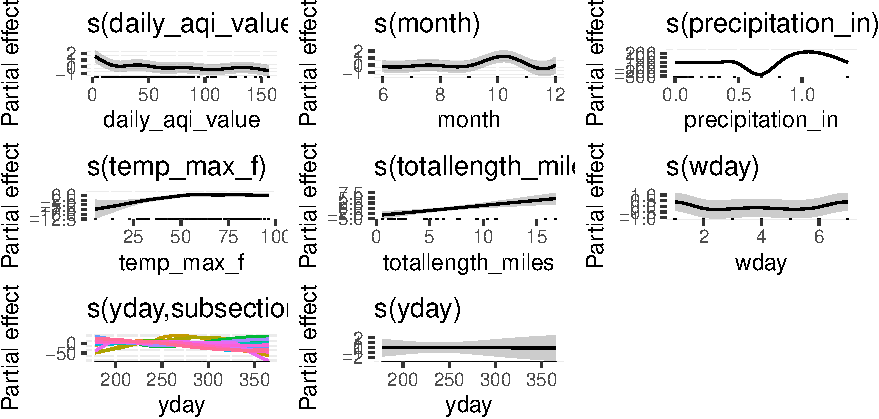
\includegraphics[width=\linewidth]{Statistical-Analysis--Prediction-of-Trail-Use-in-Bridger-Mountains_files/figure-latex/modelGS-draw-1} \caption{Global function (\texttt{s(yday)}) and group-specific deviations from the global function (\texttt{s(yday, subsection)}) for \texttt{gamm\_modGS\_ARMA\_sub)}. }\label{fig:modelGS-draw}
\end{figure}

\begin{figure}

{\centering \includegraphics[width=1\linewidth]{../figures/high_pred_modGS} 

}

\caption{Predicted trail use count values (lines) versus observed trail use (points) for each high-use trail subsection, based on model \emph{GS}.}\label{fig:high-pred-GS}
\end{figure}

\begin{figure}

{\centering \includegraphics[width=1\linewidth]{../figures/low_pred_modGS} 

}

\caption{Predicted trail use count values (lines) versus observed trail use (points) for each low-use trail subsection, based on model \emph{GS}.}\label{fig:low-pred-GS}
\end{figure}

\begin{Shaded}
\begin{Highlighting}[]
\CommentTok{\#add the predicted values from the model }
\NormalTok{allTrail\_GS\_pred }\OtherTok{\textless{}{-}} \FunctionTok{transform}\NormalTok{(allTrail\_G, }
                      \AttributeTok{mod\_GS =} \FunctionTok{predict}\NormalTok{(gamm\_modGS\_AR1}\SpecialCharTok{$}\NormalTok{gam, }
                                      \AttributeTok{type =} \StringTok{"response"}\NormalTok{))}

\FunctionTok{ggplot}\NormalTok{(allTrail\_GS\_pred, }\FunctionTok{aes}\NormalTok{(}\AttributeTok{x=}\NormalTok{mod\_GS, }\AttributeTok{y=}\NormalTok{max.camera)) }\SpecialCharTok{+}
  \FunctionTok{facet\_wrap}\NormalTok{(}\SpecialCharTok{\textasciitilde{}}\NormalTok{subsectionF, }\AttributeTok{ncol=} \DecValTok{3}\NormalTok{) }\SpecialCharTok{+}
  \FunctionTok{geom\_point}\NormalTok{(}\AttributeTok{alpha=}\FloatTok{0.3}\NormalTok{, }\FunctionTok{aes}\NormalTok{(}\AttributeTok{color =}\NormalTok{ trailname)) }\SpecialCharTok{+}
  \FunctionTok{scale\_color\_manual}\NormalTok{(}\AttributeTok{name =} \StringTok{"Trail"}\NormalTok{, }\AttributeTok{values =}\NormalTok{ colors) }\SpecialCharTok{+}
  \FunctionTok{geom\_abline}\NormalTok{() }\SpecialCharTok{+}
  \FunctionTok{theme}\NormalTok{(}\AttributeTok{legend.position=}\StringTok{"none"}\NormalTok{) }\SpecialCharTok{+}
  \FunctionTok{labs}\NormalTok{(}\AttributeTok{x=}\StringTok{"Predicted count"}\NormalTok{, }\AttributeTok{y=}\StringTok{"Observed count"}\NormalTok{)}
\end{Highlighting}
\end{Shaded}

\begin{figure}

{\centering 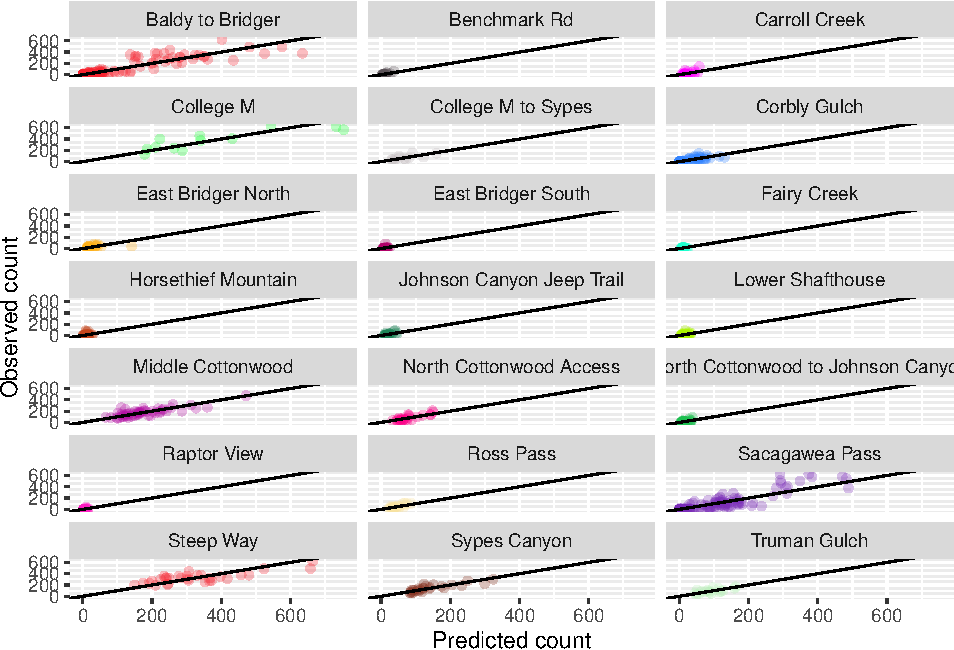
\includegraphics[width=1\linewidth]{Statistical-Analysis--Prediction-of-Trail-Use-in-Bridger-Mountains_files/figure-latex/modGS-pred-observed-1} 

}

\caption{Assuming a well-fitted model GS, we would expect all trail subsections exhibiting similar patterns of dispersion around the 1-1 line (and as we are assuming the data is Poisson, the variance around the mean should equal the mean).}\label{fig:modGS-pred-observed}
\end{figure}

\hypertarget{single-common-smoother-plus-group-level-smoothers-with-differing-wiggliness-model-gi}{%
\subsection{Single common smoother plus group-level smoothers with differing wiggliness (Model GI)}\label{single-common-smoother-plus-group-level-smoothers-with-differing-wiggliness-model-gi}}

In this model class each group-specific smoother is permitted to have its own smoothing parameter and hence its own level of wiggliness. These models take the longest to run (as there are more smoothing parameters to estimate), but is useful if the different groups (here, trail subsections) differ in how `wiggly' they are.

There are two major differences in how model GS was specified:

\begin{enumerate}
\def\labelenumi{\arabic{enumi}.}
\item
  Explicit inclusion of a random effect for the intercept (the bs=``re'' term).
\item
  Specify m=1 instead of m=2 for the group-level smoothers. This allows for the marginal TPRS basis for relevent terms will penalize the squared first derivative of the function, rather than the second derivative. The aim is to reduce colinearity between the global smoother and the group-specific terms.
\end{enumerate}

This approach in R looks like:

\begin{Shaded}
\begin{Highlighting}[]
\NormalTok{ gamm\_modGI\_AR1 }\OtherTok{\textless{}{-}} \FunctionTok{gamm}\NormalTok{(max.camera }\SpecialCharTok{\textasciitilde{}}
                           \FunctionTok{s}\NormalTok{(yday, }\AttributeTok{m=}\DecValTok{2}\NormalTok{, }\AttributeTok{bs=}\StringTok{"cc"}\NormalTok{) }\SpecialCharTok{+}
                           \FunctionTok{s}\NormalTok{(yday, }\AttributeTok{by =}\NormalTok{ subsectionF,}
                             \AttributeTok{m=}\DecValTok{1}\NormalTok{, }\AttributeTok{bs=}\StringTok{"cc"}\NormalTok{) }\SpecialCharTok{+}
                           \FunctionTok{s}\NormalTok{(subsectionF,}
                             \AttributeTok{bs=}\StringTok{"re"}\NormalTok{,}
                             \CommentTok{\# by = trailnameF,}
                             \AttributeTok{k=}\DecValTok{21}\NormalTok{) }\SpecialCharTok{+}
                           \CommentTok{\# trailnameF +}
                           \FunctionTok{s}\NormalTok{(month, }\AttributeTok{bs =} \StringTok{"cc"}\NormalTok{,  }\AttributeTok{k =} \DecValTok{7}\NormalTok{) }\SpecialCharTok{+}
                           \FunctionTok{s}\NormalTok{(wday,}
                             \AttributeTok{bs =} \StringTok{"cc"}\NormalTok{, }\AttributeTok{k =} \DecValTok{7}\NormalTok{) }\SpecialCharTok{+}
                           \FunctionTok{s}\NormalTok{(daily\_aqi\_value) }\SpecialCharTok{+}
                           \FunctionTok{s}\NormalTok{(temp\_max\_f) }\SpecialCharTok{+}
                           \FunctionTok{s}\NormalTok{(precipitation\_in, }\AttributeTok{k =} \DecValTok{5}\NormalTok{) }\SpecialCharTok{+}
                          \FunctionTok{s}\NormalTok{(totallength\_miles) }\SpecialCharTok{+} 
\NormalTok{                        total\_traveltime }\SpecialCharTok{+}
\NormalTok{                            max.count,}
                          \AttributeTok{knots =} \FunctionTok{list}\NormalTok{(}\AttributeTok{yday =} \FunctionTok{c}\NormalTok{(}\DecValTok{0}\NormalTok{,}\DecValTok{365}\NormalTok{),}
                                       \AttributeTok{month =} \FunctionTok{c}\NormalTok{(}\DecValTok{0}\NormalTok{, }\DecValTok{13}\NormalTok{)),}
                           \AttributeTok{correlation =} \FunctionTok{corAR1}\NormalTok{(}\AttributeTok{form =} \SpecialCharTok{\textasciitilde{}}\NormalTok{yday}\SpecialCharTok{|}\NormalTok{subsectionF),}
                         \AttributeTok{data =}\NormalTok{ allTrail,}
                         \AttributeTok{family =}\NormalTok{ poisson)}
\end{Highlighting}
\end{Shaded}

When including a by-variable smooth, you are allowing for different smoothness parameters for each level of \texttt{subsectionF}.

Here, we present the summary and diagnostic plots for model GI with an AR1 temporal structure.

\begin{verbatim}
##                    Model df      AIC       BIC    logLik   Test  L.Ratio p-value
## gamm_modGI$lme         1 36 126685.2 126864.08 -63306.58                        
## gamm_modGI_AR1$lme     2 37  66969.6  67153.49 -33447.80 1 vs 2 59717.57  <.0001
\end{verbatim}

The summary now includes all the different day of year (\texttt{yday}) by trail subsection (\texttt{subsectionF}) parameters.

\begin{verbatim}
## 
## Family: poisson 
## Link function: log 
## 
## Formula:
## max.camera ~ s(yday, m = 2, bs = "cc") + s(yday, by = subsectionF, 
##     m = 1, bs = "cc") + s(subsectionF, bs = "re", k = sub.number) + 
##     s(month, bs = "cc", k = 7) + s(wday, bs = "cc", k = 7) + 
##     s(daily_aqi_value) + s(temp_max_f) + s(precipitation_in, 
##     k = 5) + s(totallength_miles) + total_traveltime + max.count
## 
## Parametric coefficients:
##                    Estimate Std. Error t value Pr(>|t|)    
## (Intercept)       0.8992494  0.3759070   2.392   0.0169 *  
## total_traveltime -0.0401890  0.0082482  -4.872 1.29e-06 ***
## max.count         0.0116742  0.0005485  21.282  < 2e-16 ***
## ---
## Signif. codes:  0 '***' 0.001 '**' 0.01 '*' 0.05 '.' 0.1 ' ' 1
## 
## Approximate significance of smooth terms:
##                                                             edf Ref.df        F  p-value    
## s(yday)                                               7.127e+00  8.000  994.511  < 2e-16 ***
## s(yday):subsectionFBaldy to Bridger                   6.162e+00  8.000 1195.664  < 2e-16 ***
## s(yday):subsectionFBenchmark Rd                       2.175e+00  5.000  358.320 0.049930 *  
## s(yday):subsectionFCarroll Creek                      1.416e+00  5.000    3.342 0.787660    
## s(yday):subsectionFCollege M                          3.800e+00  5.000 1078.270 1.86e-05 ***
## s(yday):subsectionFCollege M to Sypes                 3.563e+00  5.000  537.253 7.88e-07 ***
## s(yday):subsectionFCorbly Gulch                       7.504e+00  8.000 1062.789  < 2e-16 ***
## s(yday):subsectionFEast Bridger North                 1.237e-04  6.000    0.000 0.416870    
## s(yday):subsectionFEast Bridger South                 3.047e+00  6.000  872.823 6.56e-05 ***
## s(yday):subsectionFFairy Creek                        3.310e+00  5.000 1191.535 0.000547 ***
## s(yday):subsectionFHorsethief Mountain                8.804e-05  6.000    0.000 0.454800    
## s(yday):subsectionFJohnson Canyon Jeep Trail          2.233e+00  5.000  418.336 0.005384 ** 
## s(yday):subsectionFLower Shafthouse                   2.883e+00  7.000  185.441 0.001892 ** 
## s(yday):subsectionFMiddle Cottonwood                  4.154e+00  5.000 2127.067 5.46e-05 ***
## s(yday):subsectionFNorth Cottonwood Access            4.338e+00  5.000 1498.815 0.001054 ** 
## s(yday):subsectionFNorth Cottonwood to Johnson Canyon 4.663e+00  6.000 1049.535 3.97e-06 ***
## s(yday):subsectionFRaptor View                        1.281e+00  5.000  160.742 0.053252 .  
## s(yday):subsectionFRoss Pass                          1.198e+00  4.000  211.833 4.21e-05 ***
## s(yday):subsectionFSacagawea Pass                     7.971e+00  8.000 3361.353  < 2e-16 ***
## s(yday):subsectionFSteep Way                          4.624e+00  5.000  122.084 0.004566 ** 
## s(yday):subsectionFSypes Canyon                       1.308e-05  5.000    0.000 0.391803    
## s(yday):subsectionFTruman Gulch                       3.688e+00  5.000  651.198 0.009058 ** 
## s(subsectionF)                                        4.968e+00 19.000    4.635  < 2e-16 ***
## s(month)                                              3.623e+00  5.000   11.556  < 2e-16 ***
## s(wday)                                               4.976e+00  5.000  461.824  < 2e-16 ***
## s(daily_aqi_value)                                    8.912e+00  8.912  170.707  < 2e-16 ***
## s(temp_max_f)                                         8.724e+00  8.724 1039.786  < 2e-16 ***
## s(precipitation_in)                                   3.744e+00  3.744  103.796  < 2e-16 ***
## s(totallength_miles)                                  1.000e+00  1.000   39.097  < 2e-16 ***
## ---
## Signif. codes:  0 '***' 0.001 '**' 0.01 '*' 0.05 '.' 0.1 ' ' 1
## 
## R-sq.(adj) =  0.843   
##   Scale est. = 1         n = 1064
\end{verbatim}

Figure \ref{fig:modelGI-draw} shows a subsample of the group-specific smoothers from this model. Some trail subsections (e.g., East Bridger South) have very similar shapes to the global smoother. Others do differ from this trend with lower trail use earlier in the year and higher in later times (e.g., Baldy to Bridger) or a mix of variations from the global trend (e.g., Corbly Gulch, Sacagawea Pass, Steep Way).

\begin{figure}

{\centering 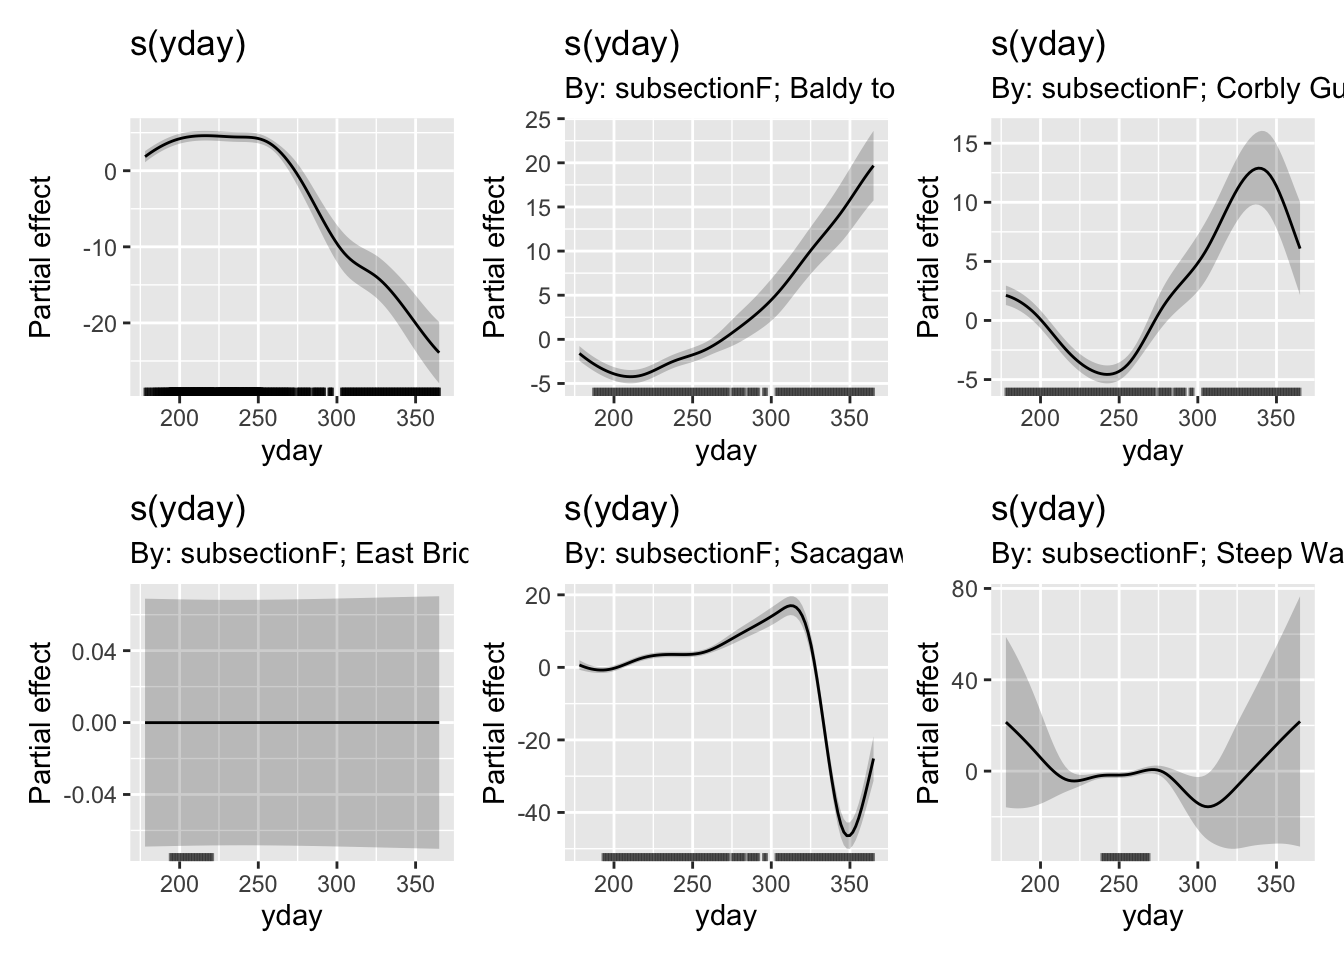
\includegraphics{Statistical-Analysis--Prediction-of-Trail-Use-in-Bridger-Mountains_files/figure-latex/modelGI-draw-1} 

}

\caption{Subsection of partial effect plots for model \emph{GI}.}\label{fig:modelGI-draw}
\end{figure}

Figures \ref{fig:modelGI-tsDiag1} and \ref{fig:modelGI-tsDiag2} shows that model GI is the first and only model to fully capture the temporal autocorrelation (through the AR1 structure). There is only slight evidence for overdispersion (Figures \ref{fig:modelGI-rootogram} and \ref{fig:modGI-pred-observed}) which seems most likely due to a slightly zero-inflated distribution.

\begin{figure}

{\centering 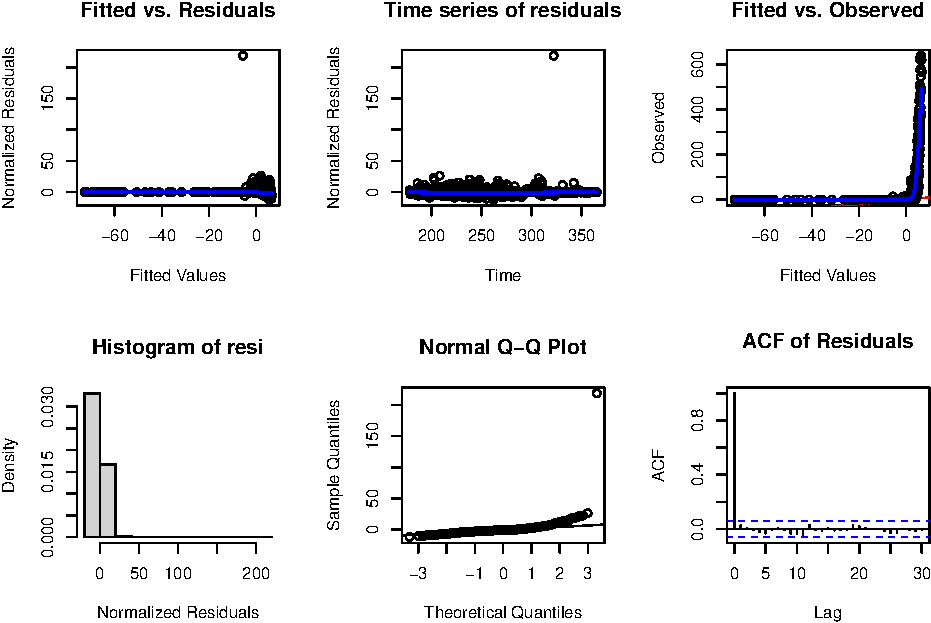
\includegraphics[width=1\linewidth]{Statistical-Analysis--Prediction-of-Trail-Use-in-Bridger-Mountains_files/figure-latex/modelGI-tsDiag1-1} 

}

\caption{Times series diagnosis plots for model \emph{GI}.}\label{fig:modelGI-tsDiag1}
\end{figure}

\begin{figure}

{\centering 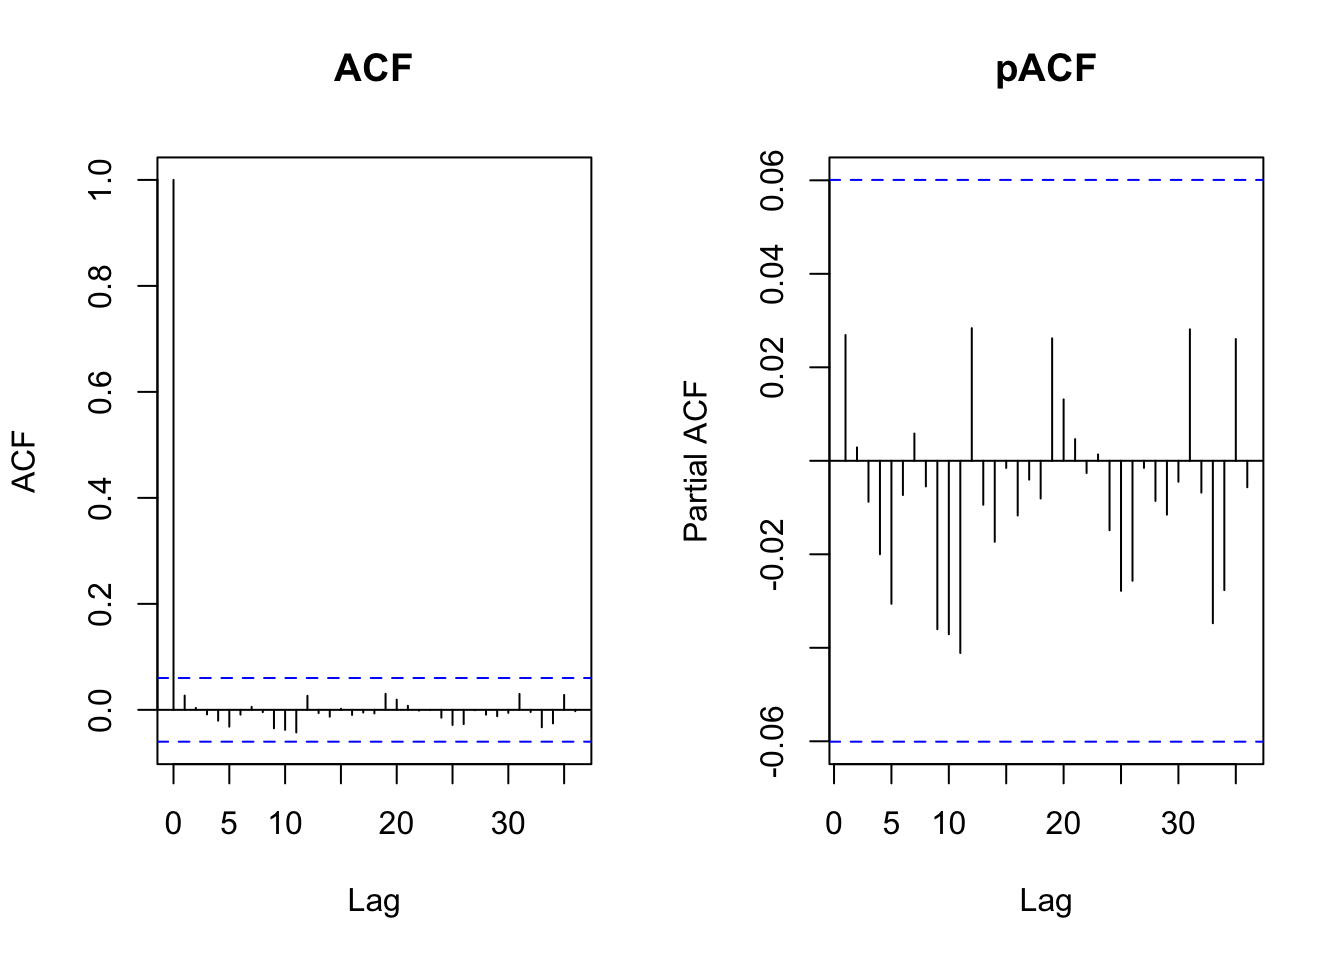
\includegraphics{Statistical-Analysis--Prediction-of-Trail-Use-in-Bridger-Mountains_files/figure-latex/modelGI-tsDiag2-1} 

}

\caption{Times series ACF/pACF diagnosis plots for model \emph{GI}.}\label{fig:modelGI-tsDiag2}
\end{figure}

\begin{Shaded}
\begin{Highlighting}[]
\NormalTok{rg }\OtherTok{\textless{}{-}}\NormalTok{ gratia}\SpecialCharTok{::}\FunctionTok{rootogram}\NormalTok{(gamm\_modGI\_AR1}\SpecialCharTok{$}\NormalTok{gam)}
\FunctionTok{draw}\NormalTok{(rg)}
\end{Highlighting}
\end{Shaded}

\begin{figure}

{\centering 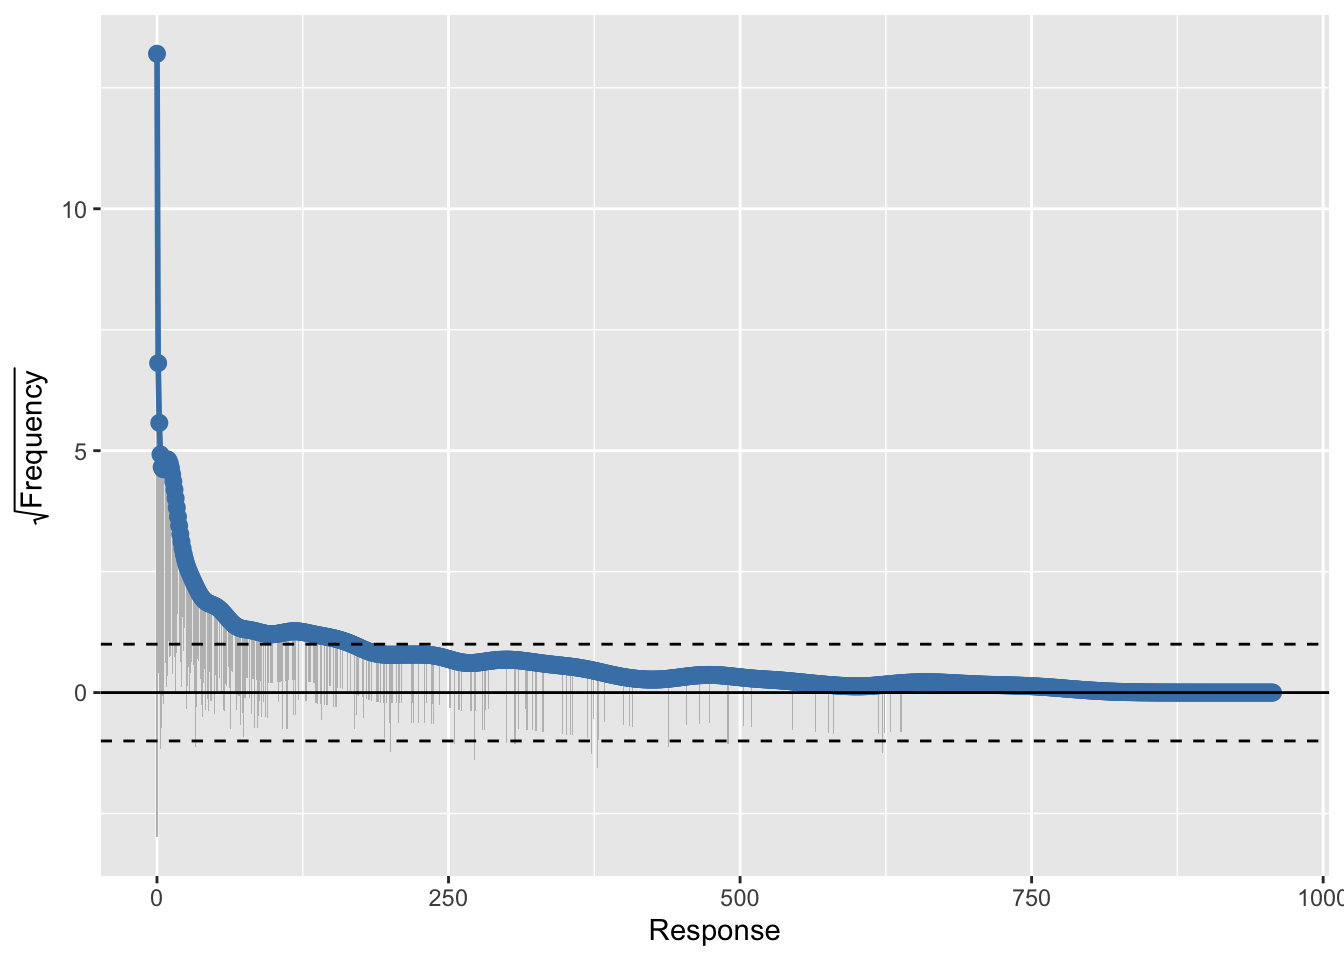
\includegraphics[width=1\linewidth]{Statistical-Analysis--Prediction-of-Trail-Use-in-Bridger-Mountains_files/figure-latex/modGI-rootogram-1} 

}

\caption{Rootogram for checking for overdispersion.}\label{fig:modGI-rootogram}
\end{figure}

\begin{Shaded}
\begin{Highlighting}[]
\CommentTok{\#add the predicted values from the model }
\NormalTok{allTrail\_GI\_pred }\OtherTok{\textless{}{-}} \FunctionTok{transform}\NormalTok{(allTrail\_G, }
                      \AttributeTok{mod\_GI =} \FunctionTok{predict}\NormalTok{(gamm\_modGI\_AR1}\SpecialCharTok{$}\NormalTok{gam, }
                                      \AttributeTok{type =} \StringTok{"response"}\NormalTok{))}

\FunctionTok{ggplot}\NormalTok{(allTrail\_GI\_pred, }\FunctionTok{aes}\NormalTok{(}\AttributeTok{x=}\NormalTok{mod\_GI, }\AttributeTok{y=}\NormalTok{max.camera)) }\SpecialCharTok{+}
  \FunctionTok{facet\_wrap}\NormalTok{(}\SpecialCharTok{\textasciitilde{}}\NormalTok{subsectionF, }\AttributeTok{ncol=} \DecValTok{3}\NormalTok{) }\SpecialCharTok{+}
  \FunctionTok{geom\_point}\NormalTok{(}\AttributeTok{alpha=}\FloatTok{0.3}\NormalTok{, }\FunctionTok{aes}\NormalTok{(}\AttributeTok{color =}\NormalTok{ trailname)) }\SpecialCharTok{+}
  \FunctionTok{scale\_color\_manual}\NormalTok{(}\AttributeTok{name =} \StringTok{"Trail"}\NormalTok{, }\AttributeTok{values =}\NormalTok{ colors) }\SpecialCharTok{+}
  \FunctionTok{geom\_abline}\NormalTok{() }\SpecialCharTok{+}
  \FunctionTok{theme}\NormalTok{(}\AttributeTok{legend.position=}\StringTok{"none"}\NormalTok{) }\SpecialCharTok{+}
  \FunctionTok{labs}\NormalTok{(}\AttributeTok{x=}\StringTok{"Predicted count"}\NormalTok{, }\AttributeTok{y=}\StringTok{"Observed count"}\NormalTok{)}
\end{Highlighting}
\end{Shaded}

\begin{figure}
\centering
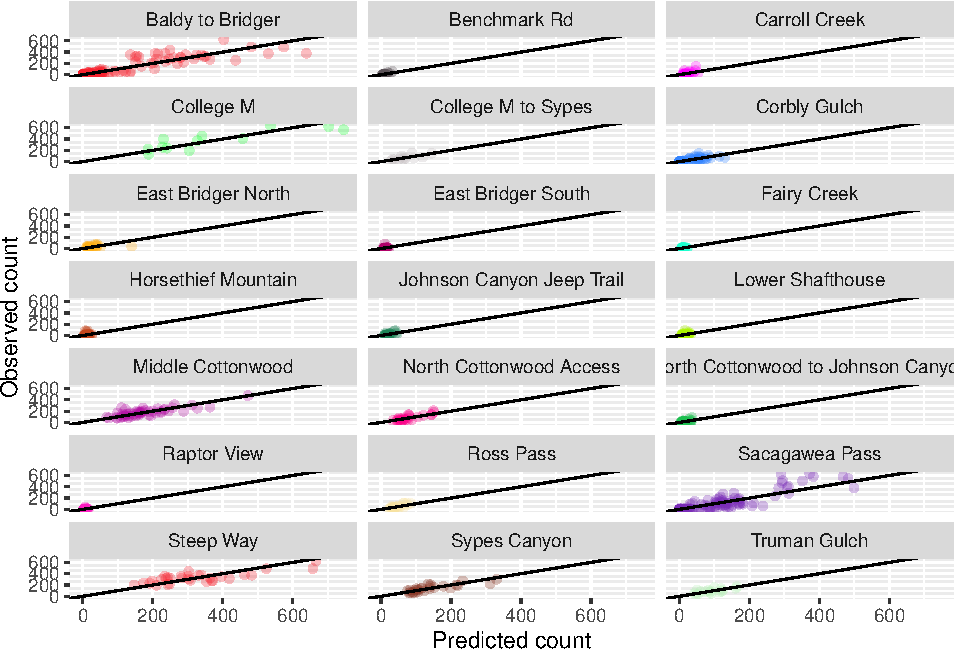
\includegraphics{Statistical-Analysis--Prediction-of-Trail-Use-in-Bridger-Mountains_files/figure-latex/modGI-pred-observed-1.pdf}
\caption{\label{fig:modGI-pred-observed}Assuming a well-fitted model GI, we would expect all trail subsections exhibiting similar patterns of dispersion around the 1-1 line (and as we are assuming the data is Poisson, the variance around the mean should equal the mean).}
\end{figure}

Figures \ref{fig:high-pred-GI} and \ref{fig:low-pred-GI} show the predictive values and observed data points for model GI.

\begin{figure}
\includegraphics[width=1\linewidth]{../figures/high_pred_modGI} \caption{Predicted trail use count values (lines) versus observed trail use (points) for each high-use trail subsection, based on model \emph{GI}.}\label{fig:high-pred-GI}
\end{figure}

\begin{figure}
\includegraphics[width=1\linewidth]{../figures/low_pred_modGI} \caption{Predicted trail use count values (lines) versus observed trail use (points) for each low-use trail subsection, based on model \emph{GI}.}\label{fig:low-pred-GI}
\end{figure}

\hypertarget{predictionforecasting}{%
\section{Prediction/Forecasting}\label{predictionforecasting}}

Up until this point we have looked at predictions for in-sample data. Effectively interpolating with our predictions. To examine the usefulness of these models for forecasting (i.e.~predicting trail use in the near future) we may look at how these models handle temporal extrapolation (i.e.~prediction outside of the range of data used to fit the models). We discussed in Section \ref{MidCotPred} that extrapolation in the GA(M)M framework can be tricky due to how the model uses splines to learn from the data via the basis functions.

Figures \ref{fig:high-compare-pred} and \ref{fig:low-compare-pred} both show predicted trail use for the best model within each G, GS, and GI for the entire year of 2021. Observed trail use counts are plotted (colored by day of week). Both Models GS and GI show improvement over Model G, which is to be expected due to increase variability between trail subsections. Some trail subsections (e.g.~Steep Way) still show unreasonably high predictions (and large error ribbons), however trails with a longer duration of observations (e.g.~Baldy to Bridger) show improvement. Several model specification choices have improved these predictions over past iterations of models (not shown). For example, the use of cyclic cubic splines for time predictor variables (\texttt{bs=\ "cc"}) allows information from winter observations late in the year to inform predictions for early in the year. Also, restricting the number of knots for \texttt{precipitation\_in} (now \(k=5\) when before it was allowed to default to \(k=10\)) has removed some odd jumps in predictions on days with high precipitation. One notable difficulty for these models across all trails is the ability to predict higher than typical trail use days.

\begin{figure}

{\centering \includegraphics[width=1\linewidth]{../figures/high_pred_compare} 

}

\caption{Predicted trail use count values (lines) versus observed trail use (points) for each high-use trail subsection over an entire year, based on each model (\emph{G}, \emph{GS}, and \emph{GI}). Observed trip counts (data points) are colored by day of the week and show the higher use on weekends. }\label{fig:high-compare-pred}
\end{figure}

\begin{figure}

{\centering \includegraphics[width=1\linewidth]{../figures/low_pred_compare} 

}

\caption{Predicted trail use count values (lines) versus observed trail use (points) for each low-use trail subsection, based on each model (\emph{G}, \emph{GS}, and \emph{GI}).}\label{fig:low-pred-compare}
\end{figure}

To be added: comparison of Middle Cottonwood predicitons for single trail model vs this joint model. Currently the single trail model also uses AllTrails data which has duplicate search view numbers for certain days. This messes with my code that combines all predictions for plotting. When fixed the plots will show that models that share data across subtrails improve predictions over models with individual trail data.

Figure \ref{fig:predict-newtrails} shows predictions from the top model within each category for trails in Bridger Mountains without deployed camera counters. All other covariate data is available for the year 2021.

\begin{figure}

{\centering 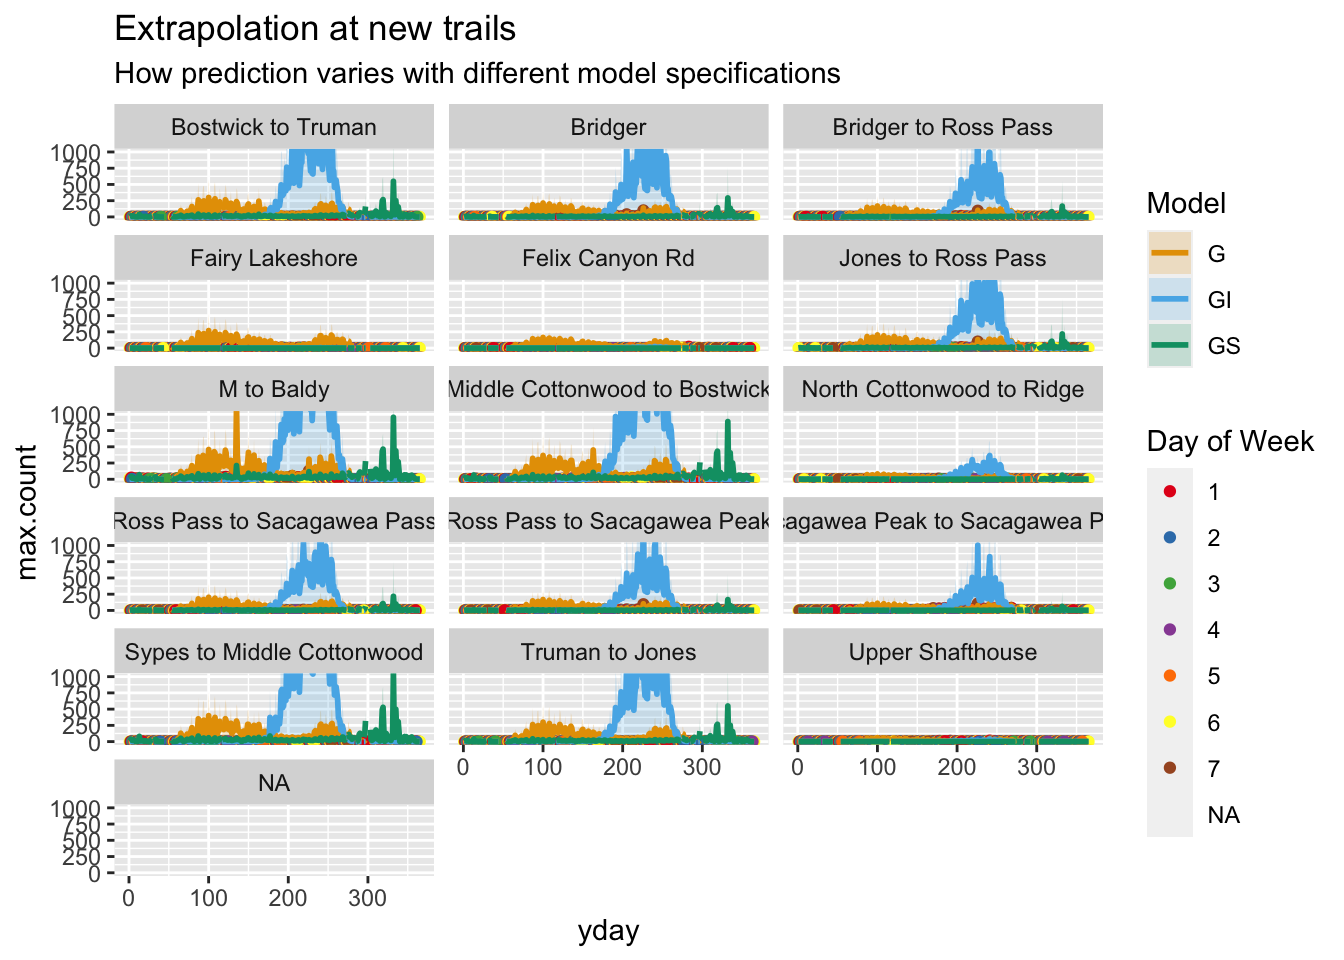
\includegraphics[width=1\linewidth]{Statistical-Analysis--Prediction-of-Trail-Use-in-Bridger-Mountains_files/figure-latex/predict-newtrails-1} 

}

\caption{Predicitons at Bridger Mountain trails without deployed camera counters.}\label{fig:predict-newtrails}
\end{figure}

To be added (hopefully) animated plots of prediction values and residuals plotted spatially. Currently these animations are super cursed and are not yet up and running.

\hypertarget{results}{%
\section{Results}\label{results}}

Comparing models based on AIC is a robust approach to comparing the different model structures. It has been shown to be an appropriate means of model comparison for models fit with \texttt{gam()}, but has not been similarly confirmed for models fit with \texttt{gamm()}. While we use this approach here, results should be taken with a grain of salt. For example, even though visual inspection of predictions of models GS and GI seem to show evidence of improvement over model G, Table \ref{tab:AICkable} does not provides evidence for including among-group functional variability. In \citet{pedersen2019hierarchical}, they caution against selecting models based purely on AIC. Instead, model selection should be based on expert subject knowledge about the system, computational time, and most importantly, the inferential goals of the study.

\begin{table}

\caption{\label{tab:AICkable}AIC table comparing model fits}
\centering
\begin{tabular}[t]{lrrr}
\toprule
Model & df & AIC & deltaAIC\\
\midrule
gamm\_modG\_ARMA\$lme & 20 & 31217 & 0\\
gamm\_modGS\_AR1\$lme & 17 & 68829 & 37612\\
gamm\_modGI\_AR1\$lme & 37 & 66970 & 35752\\
\bottomrule
\end{tabular}
\end{table}

Our goal to select the model that has the best predictive ability across various trail types. This can be checked by holding some fraction of the data out (e.g., a single trail subsection) prior to the analysis and comparing how well different models fit that data. To this end, we have left out the New World Gulch trail and fit our selected model for each type (G, GS, GI) to these out-of-sample data. To evaluate how well each model fits this new data, we calculated the total deviance of the out-of-sample data. The deviance is equal to two times the sum of the difference between the log-likelihood of the out-of-sample data (as predicted by each model) and a saturated model that has one predictor for each data point, all multiplied by the scale parameter for the family of interest. It can be interpreted similarly to the residual sum of squares for a simple linear regression (Wood, 2017a, p.~109).

To be added: get predictions for New World Gulch (currently missing trail characteristic data which is needed).

Table \ref{tab:deviance-kable} shows that both models GS and GI are better at predicting in-sample fits for all trail subsections in this analysis. While this provides additional evidence for including inter-group variability in our model, it does contradict our AIC findings.

\begin{table}

\caption{\label{tab:deviance-kable}Predictive ability for models \emph{G}, \emph{GS}, and \emph{GI} applied to the Bridger Mountain trail use dataset. Deviance values represent the total deviance of model predictions from observations. Intercept only results are for a null model with only subsection-level random effect intercepts included.}
\centering
\begin{tabular}[t]{lllll}
\toprule
\multicolumn{1}{c}{ } & \multicolumn{3}{c}{Total deviance} \\
\cmidrule(l{3pt}r{3pt}){2-4}
subsectionF & Intercept only & Model G & Model GS & Model GI\\
\midrule
Baldy to Bridger & 29338 & 6851 & 3245 & 3253\\
Benchmark Rd & 287 & 221 & 116 & 130\\
Carroll Creek & 852 & 600 & 533 & 571\\
College M & 886 & 354 & 306 & 297\\
College M to Sypes & 280 & 154 & 129 & 112\\
\addlinespace
Corbly Gulch & 6241 & 6068 & 731 & 730\\
East Bridger North & 449 & 421 & 430 & 437\\
East Bridger South & 322 & 348 & 300 & 313\\
Fairy Creek & 130 & 226 & 142 & 148\\
Horsethief Mountain & 1161 & 1261 & 1117 & 1156\\
\addlinespace
Johnson Canyon Jeep Trail & 527 & 311 & 291 & 291\\
Lower Shafthouse & 600 & 875 & 481 & 484\\
Middle Cottonwood & 1396 & 1175 & 591 & 601\\
North Cottonwood Access & 807 & 378 & 279 & 278\\
North Cottonwood to Johnson Canyon & 615 & 727 & 375 & 377\\
\addlinespace
Raptor View & 232 & 247 & 166 & 214\\
Ross Pass & 535 & 294 & 224 & 224\\
Sacagawea Pass & 29194 & 7959 & 4674 & 4648\\
Steep Way & 748 & 651 & 533 & 542\\
Sypes Canyon & 744 & 352 & 213 & 231\\
\addlinespace
Truman Gulch & 300 & 385 & 186 & 184\\
\bottomrule
\end{tabular}
\end{table}

\hypertarget{conclusions}{%
\section{Conclusions}\label{conclusions}}

The GAM framework and its extensions that allow for modelling non-linear and linear relationships between response variables and predictors with random effects and a way to account for temporal autocorrelation is a valuable tool for a statistical analysis of trail use in the Bridger Mountains. Limitations of this model includes not being able to incorporate both spatial and temporal autocorrelation without some heavy lifting required. It's not clear how to model nested random effects of trail and trail subsections in this model. Section \ref{Spatial} provides a look at an alternative model that allows for spatial correlation to be incorporated instead of temporal.

While the GAM framework for modelling is a powerful tool, it also requires a lot of modeling specification decisions. In this report we have discussed different options for model type that allows for different ways to provide a global smoother and inter-trail variation (models G, GS, and GI), the choice of basis functions and number of knots, differing ways to account for temporal correlation, and what/how many predictor variables to include. Model complexity could increase if interaction terms were to be included as well. Another complication is that while tools for diagnotics and model comparison are well developed for models fit with the \texttt{gam()} function, when we fit with the \texttt{gamm()} function (as we do in this model with our timeseries data) extra care must be taken as not all tools are appropriate in this case. Packages such as the \textbf{gratia} package which provides visulizing and diagnostic functions for GAMs is still adding functionality and will likely provide additional tools for future analyses. Even with all of this considered, this modelling framework has been shown to be a promising way to analyse recreational trail use and contains a lot of flexibility while being able to not only provide predictions at new trails/times of year but also valuable insight into trends for each predictor variable. The predictive abilities of these models will increase as additional data is made available.

With this in mind, we provide the following recommendations for future observations periods and analyses.

\begin{enumerate}
\def\labelenumi{\arabic{enumi}.}
\tightlist
\item
  It is better to have cameras deployed for longer periods of times. Year-round data for even a subset of trails will help improve predictions across all trails.
\item
  Subsections within a trail seem to capture similar data. Cameras spread across more trails may provide more information than multiple camera counters deployed along a single trail.
\item
  Multiple years of data would provide valuable information about annual trends and be helpful in forecasting trail use into the future.
\item
  If spatiotemporal correlation structure is available for future analysis then it would be helpful to consider the spatial network node/edge designations in tandem with camera placement.
\end{enumerate}

\hypertarget{TradeOff}{%
\chapter{Trade-Offs in Prediction Accuracy}\label{TradeOff}}

A secondary aim of this report is to assess tradeoffs in predictive accuracy for the statistical application. Here, we investigate several scenarios where we anticipate discrepancies in predictive abilities.

\hypertarget{high-use-versus-low-use}{%
\section{High Use versus Low Use}\label{high-use-versus-low-use}}

Due to variation in trail use across the network of trails in the Bridger Mountains we anticipate different levels of predictive ability between trails of high and low use. To provide a comparison for predictive accuracy, we first assign trails (at the subsection level) to be a ``high'' or ``low'' use trail based on expert input by Headwaters Economics. The following categories were determined:

High Use: Baldy to Bridger, Bridger, Bridger to Ross Pass, College M, M to Baldy, Middle Cottonwood, Sypes Canyon, Ross Pass to Sacagawea Peak, Sacagawea Pass, Steep Way

Low Use: Fairy Creek, Horsethief Mountain, Carroll Creek, Raptor View, College M to Sypes, Truman Gulch, East Bridger South, East Bridger North, Lower Shafthouse, Corbly Gulch, North Cottonwood to Johnson Canyon, North Cottonwood Access, Johnson Canyon Jeep Trail, Benchmark Rd

We use deviance as our chosen metric for assessing predictive accuracy. We looked at models fit with types G, GS, and GI (see Section \ref{AllTrailsAnalysis} for details) and then obtained predictions for those same (in-sample) trail subsections. To account for different number of days of observation between these two groups the calculated deviance for each model was divided by the number of days of observations to find an average deviance measure. Table @ref(tab:deviance\_highlow\_kable) shows that Model GS provided the best fit for both two groupings of trials. Additionally the deviance measure is lowest for the ``low'' use trial group. One explanation is that all models fit to these data had a difficult time predicting on days with higher than typical trail use. These events are more likely to occur on high use trails and thus the predictions for these trails will have a higher deviance overall.

\begin{table}
\centering
\begin{tabular}{lrrrr}
\toprule
\multicolumn{1}{c}{ } & \multicolumn{3}{c}{Total deviance} \\
\cmidrule(l{3pt}r{3pt}){2-4}
highlow & Intercept.only & Model.G & Model.GS & Model.GI\\
\midrule
high & 136.93 & 38.11 & 21.02 & 21.04\\
low & 21.90 & 20.55 & 9.03 & 9.28\\
\bottomrule
\end{tabular}
\end{table}

\hypertarget{places-with-different-types-of-use}{%
\section{Places with different types of use}\label{places-with-different-types-of-use}}

We also want to investigate how prediction accuracy differs in areas of varying trail use (e.g., do motorized trails differ in important ways from non-motorized trails?).

\hypertarget{motor-vehicle-use}{%
\subsection{Motor Vehicle Use}\label{motor-vehicle-use}}

\begin{table}
\centering
\begin{tabular}{lrrrr}
\toprule
\multicolumn{1}{c}{ } & \multicolumn{3}{c}{Total deviance} \\
\cmidrule(l{3pt}r{3pt}){2-4}
Motor Vehicle Use & Intercept Only & Model G & Model GS & Model GI\\
\midrule
Dirt Bikes (seasonal) & 30.81 & 28.81 & 6.29 & 6.32\\
Non-Motorized & 97.14 & 30.58 & 18.20 & 18.34\\
Wheeled OHV 50" or < & 15.48 & 11.71 & 9.33 & 9.83\\
\bottomrule
\end{tabular}
\end{table}

\hypertarget{parking-lot-size}{%
\subsection{Parking Lot Size}\label{parking-lot-size}}

\begin{table}
\centering
\begin{tabular}{lrrrr}
\toprule
\multicolumn{1}{c}{ } & \multicolumn{3}{c}{Total deviance} \\
\cmidrule(l{3pt}r{3pt}){2-4}
Parking Lot Size & Intercept Only & Model G & Model GS & Model GI\\
\midrule
L & 110.09 & 32.34 & 18.66 & 18.70\\
M & 20.83 & 16.98 & 10.64 & 11.06\\
S & 28.66 & 27.33 & 7.62 & 7.80\\
\bottomrule
\end{tabular}
\end{table}

\begin{enumerate}
\def\labelenumi{\arabic{enumi}.}
\setcounter{enumi}{2}
\tightlist
\item
  An analysis of the change in predictive accuracy as the number of trail counters used
  changes.
\end{enumerate}

\begin{itemize}
\item
  The GAMM model applied does not allow for multiple measures per unit time. In an ideal world trail counters would be deployed at as many different trails for as long as possible. Longer deployment times would help to model season and annual trends. It is possible that with more temporal data coverage we could use simpler models (i.e.~a gam or gamm approach without the need for temporal autocorrelation structure) that would save on computation time).
\item
  Need to talk about forecasting (or temporal extrapolation). If we want to forecast in the future for a specific date or time frame we really need prior observations on those intervals (i.e.~previous years). This is not unique to GAM models, predicting beyond the range of observed samples is tough.
\end{itemize}

*Can we identify trails that are ``closest'' to global smooth trend as ideal condidates for year-round cameras?

\cleardoublepage

\hypertarget{appendix-appendix}{%
\appendix}


\hypertarget{ATDataUtility}{%
\chapter{Utility of All Trails auxilary data}\label{ATDataUtility}}

Through a partnership between AllTrails and Headwaters Economics, AllTrails has provided search data for a subset of trails in the Bridger Mountains to be used as auxillary data for the Bridger Mountain trail use statistical analysis. The following trails are included in this dataset:

\begin{enumerate}
\def\labelenumi{\arabic{enumi}.}
\tightlist
\item
  Fairy Creek
\item
  College M
\item
  Bridger Ridge
\item
  Sacagawea Pass
\item
  Sypes Canyon
\item
  Truman Gulch
\item
  Corbly Gulch
\item
  Ross Pass
\item
  Middle Cottonwood
\end{enumerate}

An overview of the available AllTrials data is presented in Section \ref{ATData}. In this report we aim to investigate the utility of these data (and potential transformation of the data) as a predictor variable in the trail use analysis. We are interested in whether some transformation of the data (e.g., moving average of views or perhaps the cumulative sum of views over the preceding \(n\) days) may prove more informative than the raw data themselves.

\hypertarget{data-visualization}{%
\section{Data Visualization}\label{data-visualization}}

We start with exploring some visualizations of different data transformations. Figure @ref\{fig:AT-vis-views\} shows potential linear relationships between the different trail subsections and the untransformed number of views for each. While not all trail subsections exhibit evidence for a linear relationship (or non-linear) we do see evidence for a positive relationship with Sacagawea Pass and Sypes Way. Additional data (days of year or different trail subsections) could still hold more evidence for this relationship.

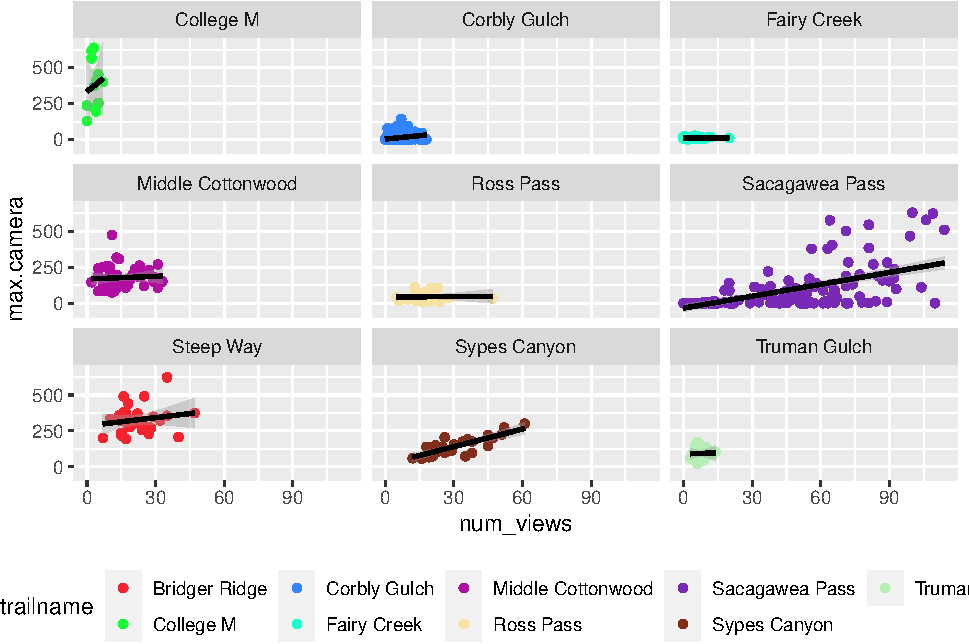
\includegraphics{Statistical-Analysis--Prediction-of-Trail-Use-in-Bridger-Mountains_files/figure-latex/AT-vis-views-1.pdf}
We started our exploration of potential data transformations with a 7-day moving average that takes the preceding 7 days to average over. This assumes the recreational users might be conducting trail searches in the week leading up to a trail use event. Figure \ref{fig:AT-vis-moving7} shows the relationship between trail use by camera counter and AllTrails searches as this 7 day moving average. There is not any increase in the number or strength of linear relationships for any of the trail subsections. Sypes Canyon no longer has quite as prominent of a positive linear relationship between the two variables. Using a shorter time frame for the moving average does not seem to provide any improvement (not shown).

\begin{figure}
\centering
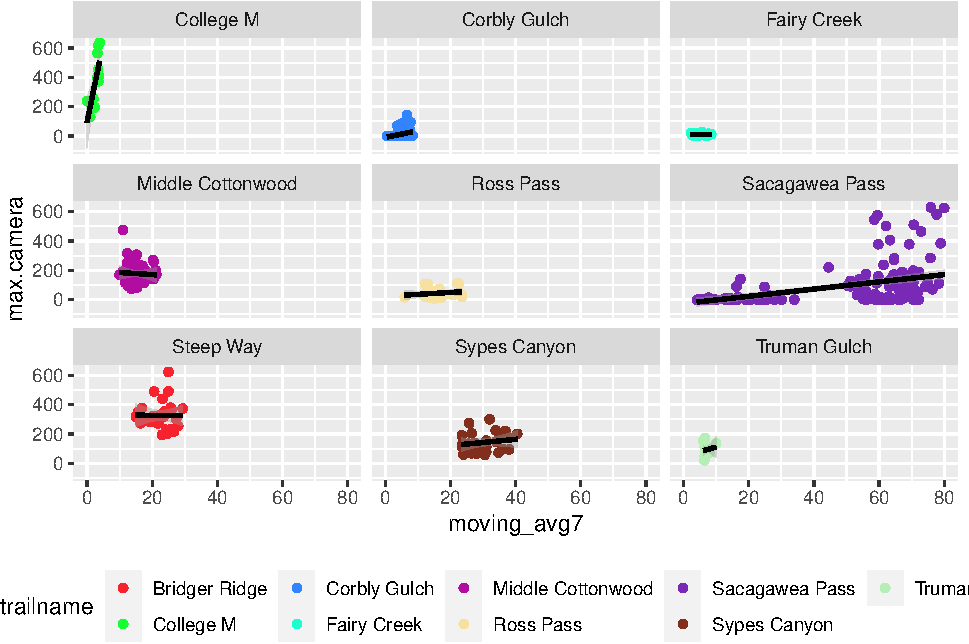
\includegraphics{Statistical-Analysis--Prediction-of-Trail-Use-in-Bridger-Mountains_files/figure-latex/AT-vis-moving7-1.pdf}
\caption{\label{fig:AT-vis-moving7}Scatterplot of trail use camera counts and AllTrails search views represented as a moving average of the number of views for the preceding seven days. Linear relationship fit (line) plotted in black.}
\end{figure}

We also explored using the cumulative sum of the previous \(n\) days. Figure \ref{fig:sumcum3} shows that this approach can show a different linear relationship compared to non-transformed search views. Both Steep Way and Middle Cottonwood now show evidence of \emph{negative} linear relationships between camera counts and search views.

What these visualizations show is that we must be careful in our choice for how we incorporate these data into our model for trail use.

\hypertarget{fitting-models}{%
\section{Fitting Models}\label{fitting-models}}

Another consideration is how to include AllTrails search data in our GAM framework with (or instead of) the Strava trip count data. We fit and compare the following models:

\begin{enumerate}
\def\labelenumi{\arabic{enumi}.}
\tightlist
\item
  Model GI with AR1 temporal correlation structure and only the Alltrail search views as the raw data.
\item
  Model GI-AR1 with only the AllTrails search data as a 7 day moving average.
\item
  Model GI-AR1 with both the Strava trip counts and the Alltrail search views as the raw data.
\item
  Model GI-AR1 with both the Strava trip counts and the Alltrail search views as a 3 day moving average.
\end{enumerate}

\hypertarget{comparing-models}{%
\section{Comparing Models}\label{comparing-models}}

We compared models using \texttt{anova} and the model with only the raw AllTrails search view counts had the lowest AIC.

\begin{verbatim}
##                                   Model df      AIC      BIC    logLik   Test  L.Ratio p-value
## gamm_modGI_AR1_searchOnly_raw$lme     1 26  20412.5  20524.2  -10180.2                        
## gamm_modGI_AR1_Both_MA3$lme           2 27  13059.8  13175.9   -6502.9 1 vs 2   7354.6  <.0001
## gamm_modGI_AR1_StravaOnly$lme         3 26 761319.9 761431.6 -380633.9 2 vs 3 748262.0  <.0001
\end{verbatim}

A look at deviance in these model predictions (Table \ref{tab:ATdeviance-kable}) shows a lot of variation between trails for the lowest amount of deviance.

\begin{table}

\caption{\label{tab:ATdeviance-kable}Predictive ability for models examining inclusion of AllTrails and Strava Metro data applied to the subsection of Bridger Mountain trail use dataset where both predictor variables are available.}
\centering
\begin{tabular}[t]{llll}
\toprule
\multicolumn{1}{c}{ } & \multicolumn{3}{c}{Total deviance} \\
\cmidrule(l{3pt}r{3pt}){2-4}
subsectionF & Model GI-AT-Raw & Model GI-Both-MA3 & Model GI-Strava\\
\midrule
College M & 205 & 251 & 305\\
Corbly Gulch & 756 & 719 & 721\\
Fairy Creek & 135 & 143 & 140\\
Middle Cottonwood & 627 & 547 & 623\\
Ross Pass & 209 & 263 & 219\\
\addlinespace
Sacagawea Pass & 3485 & 3565 & 4294\\
Steep Way & 964 & 624 & 589\\
Sypes Canyon & 248 & 182 & 200\\
Truman Gulch & 225 & 216 & 179\\
\bottomrule
\end{tabular}
\end{table}

Figure \ref{fig:ATplot-compare} shows the variation in predictions when fitting models with different auxiliary data included.

\begin{figure}

{\centering 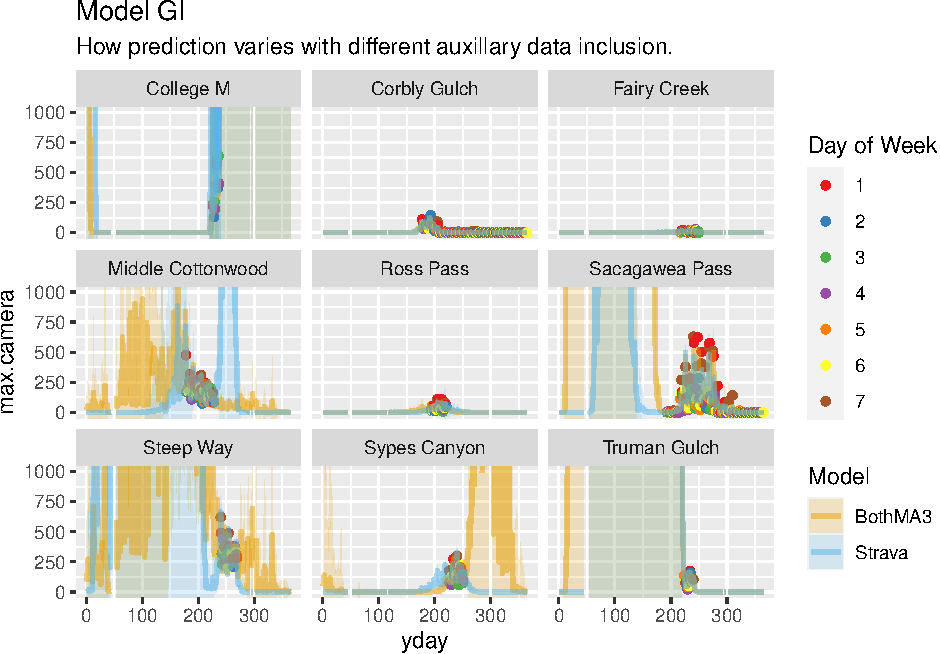
\includegraphics[width=1\linewidth]{Statistical-Analysis--Prediction-of-Trail-Use-in-Bridger-Mountains_files/figure-latex/ATplot-compare-1} 

}

\caption{Predicted trail use count values (lines) versus observed trail use (points) for each trail subsection, based on each model (Strava only with raw counts, both AllTrails and Strava with 3-day moving average, and Strava only).}\label{fig:ATplot-compare}
\end{figure}

\hypertarget{takeaway-conclusion}{%
\section{Takeaway Conclusion}\label{takeaway-conclusion}}

In our initial investigation of the AllTrails search views data we found evidence of a positive linear relationship with trail use (as camera counts) for only a few trails. We have shown evidence for including some form of AllTrails search views data in tandem with the Strava Metro provided daily trip counts in our model to improve predictive abilities. However, in our current approach, which fits a HGAMM to 21 different trail subsections, we would need AllTrails search data for all included trails. This model is unable to handle any missing covariate values. We do included AllTrails searches as the raw number of views in our Middle Cottonwood only approach (Section \ref{MidCot}) but it was not a significant linear term.

\hypertarget{Spatial}{%
\chapter{Spatial Network Generalized Additive Mixture Model}\label{Spatial}}

\begin{verbatim}
## Reading layer `bridger_trails_elev' from data source 
##   `/Users/mlbartley/Documents/Consulting/Headwaters Economics/HE-TrailUse-R/data/raw/bridger_trails_elev' 
##   using driver `ESRI Shapefile'
## Simple feature collection with 47 features and 18 fields
## Geometry type: MULTILINESTRING
## Dimension:     XYM
## Bounding box:  xmin: -111.0979 ymin: 45.54056 xmax: -110.8828 ymax: 46.04659
## m_range:       mmin: -1.797693e+308 mmax: 20.16198
## Geodetic CRS:  NAD83
\end{verbatim}

\hypertarget{overview-of-potential-model}{%
\section{Overview of Potential Model}\label{overview-of-potential-model}}

During our research into potential models for use in this statistical analysis we explored many options that ended up not being used in this report. One such model is presented here as it may prove more useful in future analyses.

We provided an overview of generalized additive models in Section \ref{Models} and in our analysis use a hierarchical generalized additive model with various temporal correlation structures to fit our trail use data. One drawback of this model is the difficulty of accounting for potential spatial correlation. The Bridger Mountains are home to a complex spatial network of trails some of which we have subdivided into subsections for this analysis. Several trails can be accessed by multiple trailheads, others are more traditional out-and-back or loops. It is a reasonable to assume that trail use would be more similar along subsections of a single trail and possibly between trails that are located closer together. Currently, we account for the random effect of subsection (\texttt{subsectionF}) in our models but we are unable to nest subsection within trail or include information about the overall spatial network.

Spatial network GAMs are another extension of the overall GAM framework that allows for the inclusion of a spatial network in a GAM approach that is used to create a spatial correlation structure in the model. Unfortunately, this is not currently an off-the-shelf way to also incorporate a \textbf{temporal} correlation structure. A bespoke spatiotemporal correlation structure could potentially created, but that is currently beyond the scope of this analysis. For the Bridger Mountain trail use statistical analysis it was determined that accounting for temporal correlation while including subsection as a random effect was the best way forward. We include an example of how to fit the spatial network model here in case future work may find it useful.

An overview of spatial network GAMs and two case studies with associated R code for analysis and plots are available at: \url{https://github.com/nick-gauthier/gam-networks}

\hypertarget{data-used-2}{%
\section{Data used}\label{data-used-2}}

The spatial data GAM requires the data be organized as a spatial network structure that includes (1) a network of ``node'' locations that mark the start and end locations of the different trail subsections and (2) the response and predictor variables with columns with location ``edges'' defined by ``to'' and ``from'' columns. For many spatial networks, these edges and nodes are easily defined. For example, towns as nodes and roads between them as edges. However, for a recreational trail network the edges are more clearly defined and the placement of nodes can require more thought. While the overall start and end nodes of an out-and-back trail might be easy to also define, other trails that branch and loop can prove more difficult. Spatial delineation of trails into subsections was decided by Headwaters Economics.

\hypertarget{model-fit}{%
\section{Model Fit}\label{model-fit}}

We fit this spatial GAM model using a correlation structure for symmetric relational data from the \textbf{corMLPE} package.

\hypertarget{model-diagnostics}{%
\section{Model Diagnostics}\label{model-diagnostics}}

The summary output for this \texttt{gamm} object shows an adjusted R-sq of 0.79 and a non-significant parametric term, \texttt{total\_traveltime}.

A look at plots (see Figures \ref{fig:mod-diagnoses} and \ref{fig:mod-acfpacf}) that provide insight into the presence of temporal dependence remaining after the model is fit shows a high degree of temporal autocorrelation.

We have included additional diagnostic plots, however no additional issues are apparent beyond the temporal correlation.

\hypertarget{model-compare}{%
\section{Model Compare}\label{model-compare}}

This model includes all trail subsections, even ones with overlapping information about Bridger Rider, for example. So we are unable to directly compare this model with those used with only a single Bridger Ridge subsection as in models G, GS, and GI. However we determined that the amount of temporal autocorrelation was too high to use this model in our statistical analysis. Should a way to implement a combined spatiotemporal correlation strucutre is developed, we choose to move forward with a \texttt{gamm} approach with temporal autocorrelation structure and trail subsection as a random effect.

  \bibliography{book.bib,packages.bib}

\end{document}
